\documentclass[11pt, a4paper, twoside]{memoir}		

%%%% PREAMBLE

% TEXT

\usepackage{libertine}									% Font
\usepackage{libertinust1math}							% Math font
\usepackage[scaled=0.8]{beramono}						% Monospace font

\usepackage[T1]{fontenc}                                % Makes it possible to use glyphs like "o etc
\usepackage[UKenglish]{babel}							% Hyphenation according to UK rules


%%%%%%%%%%%%%%%%%%%%%%%%%%%%%%%%%%%%%%%%%%%%%%%%%%%%%%%%%%%%%%%%%%%%%%%%%%%%%%%%%%%%%%
% MATH
 
\usepackage{amsmath, amsfonts, amsthm, bm}
\usepackage{mathabx}									% for \bigtimes for cartesian products
\DeclareMathOperator\erf{erf}  							% error function as \erf

%%%%%%%%%%%%%%%%%%%%%%%%%%%%%%%%%%%%%%%%%%%%%%%%%%%%%%%%%%%%%%%%%%%%%%%%%%%%%%%%%%%%%%
% LINKS, REFERENCES, CITING ETC

\usepackage[colorlinks=false,hidelinks,pdfpagelabels]{hyperref}
\hypersetup{bookmarks=true}
\usepackage[noabbrev]{cleveref}		% Makes clever referencing using \cref possible.

%%%%%%%%%%%%%%%%%%%%%%%%%%%%%%%%%%%%%%%%%%%%%%%%%%%%%%%%%%%%%%%%%%%%%%%%%%%%%%%%%%%%%%
% STYLE

\renewcommand{\cftchapterfont}{\normalfont}				% changes the font of sections in the TOC
\renewcommand{\cftchapterpagefont}{\normalfont}			% changes the font of sections in the TOC
\renewcommand*{\cftchapterleader}{\normalfont\cftdotfill{\cftsectiondotsep}}		% add dotted line for chapters to TOC

\DisemulatePackage{setspace}							% makes setspace compatible with memoir
\usepackage[labelfont={bf},textfont=it]{caption}		% makes captions bold + italic
\usepackage{setspace}									% increase line spacing
\captionsetup{font={stretch=1.25}}      				% change 1.25 for figures and tables
\renewcommand{\baselinestretch}{1.25}					% increase line spacing such that inline formulae fit better


\makechapterstyle{carsten}{%
	\setlength\beforechapskip{0pt}
	\setlength\midchapskip{0pt}
	\setlength\afterchapskip{40pt}
	\renewcommand\chapnamefont{%
		\normalfont\centering\large\scshape\MakeLowercase}
	\renewcommand\chapnumfont{%
		\normalfont\centering\fontsize{60pt}{0pt}\selectfont}
	\renewcommand\chaptitlefont{%
		\normalfont\HUGE\bfseries\centering}
	\renewcommand\printchaptername{%
		\marginpar{\chapnamefont{\@chapapp}}}
	\renewcommand\chapternamenum{}
	\renewcommand\printchapternum{%
		\marginpar{\chapnumfont\thechapter}}
}

% PAGE MARGINS
\usepackage{geometry} 									% for setting other page margins in title page
\setulmarginsandblock{3cm}{3cm}{*}		
\setlrmarginsandblock{2cm}{4cm}{*}
\checkandfixthelayout


\usepackage{titlesec}				
\titlespacing*{\section}{0pt}{1cm}{.5cm}  				% specificeren ruimte rondom sections, {left}{above}{under}


\usepackage[bottom]{footmisc} 							% sets footnotes to bottom of page



%% Floats & captions

\usepackage{subcaption} 								% makes subtables possible



\theoremstyle{plain}
\newtheorem{theorem}{Theorem}[chapter] 					% reset theorem numbering for each chapter
\newtheorem{definition}[theorem]{Definition} 			% definition numbers are dependent on theorem numbers
\newtheorem{example}[theorem]{Example} 					% same for example numbers

\def\code#1{\texttt{#1}}                                % Redefine \code command for mono-spaced text


%%%%%%%%%%%%%%%%%%%%%%%%%%%%%%%%%%%%%%%%%%%%%%%%%%%%%%%%%%%%%%%%%%%%%%%%%%%%%%%%%%%%%%
% FIGURES

\usepackage{graphicx}


%%%%%%%%%%%%%%%%%%%%%%%%%%%%%%%%%%%%%%%%%%%%%%%%%%%%%%%%%%%%%%%%%%%%%%%%%%%%%%%%%%%%%%
% TIKZ

\usepackage{tikz}
\usetikzlibrary{quotes,angles}
\usepackage{pgfplots}

% Define dotted pattern to fill nodes
\usetikzlibrary{arrows,patterns}
\pgfdeclarepatternformonly{soft crosshatch}{\pgfqpoint{-1pt}{-1pt}}{\pgfqpoint{4pt}{4pt}}{\pgfqpoint{3pt}{3pt}}%
{
	\pgfsetstrokeopacity{0.3}
	\pgfsetlinewidth{0.4pt}
	\pgfpathmoveto{\pgfqpoint{3.1pt}{0pt}}
	\pgfpathlineto{\pgfqpoint{0pt}{3.1pt}}
	\pgfpathmoveto{\pgfqpoint{0pt}{0pt}}
	\pgfpathlineto{\pgfqpoint{3.1pt}{3.1pt}}
	\pgfusepath{stroke}
}


%%%%%%%%%%%%%%%%%%%%%%%%%%%%%%%%%%%%%%%%%%%%%%%%%%%%%%%%%%%%%%%%%%%%%%%%%%%%%%%%%%%%%%
% OTHER
\newcommand\todo[1]{\textcolor{red}{#1}}



\newcommand\X{[X]}
\newcommand\Y{[Y]}
\newcommand\Yi{[Y_i]}
\newcommand\XX{\mathit{[XX]}}
\newcommand\YY{\mathit{[YY]}}
\newcommand\XY{\mathit{[XY]}}
\newcommand\YZ{\mathit{[YZ]}}
\newcommand\ZY{\mathit{[ZY]}}
\newcommand\XZ{\mathit{[XZ]}}
\newcommand\WX{\mathit{[WX]}}
\newcommand\YW{\mathit{[YW]}}
\newcommand\XYZ{\mathit{[XYZ]}}
\newcommand\XYX{\mathit{[XYX]}}
\newcommand\XYY{\mathit{[XYY]}}
\newcommand\XXX{\mathit{[XXX]}}
\newcommand\XYZW{\mathit{[^XY^Z_W]}}

\renewcommand{\Re}{\text{}\operatorname{Re}}
\renewcommand{\Im}{\text{}\operatorname{Im}}

% Define bibliography style with biblatex, should be compiled with Biber. trad-abbrv tries to copy the abbrv style and then some extra arguments are needed
\usepackage[style=trad-abbrv, sorting=none, doi=false, isbn=false, url=false, eprint=false]{biblatex} 
\addbibresource{references.bib}
\addbibresource{email.bib}
\renewbibmacro{in:}{}
\DeclareFieldFormat{pages}{#1}
\DeclareFieldFormat[article,incollection,unpublished]{title}{#1}



\begin{document}
	

\newcommand\thesispage{\normalfont \thepage}


%%%%%%%%%%%%%% CUSTOM PAGE STYLE %%%%%%%%%%%%%%%%%%%%%%%%
% Here the headers and footers are defined

\setlength{\headheight}{\baselineskip}
\setlength{\headwidth}{\textwidth\marginparsep+0.5\marginparwidth}
\makepagestyle{carsten}
\createmark{chapter}{both}{nonumber}{}{}
\makerunningwidth{carsten}{\headwidth}
\makeheadposition{carsten}{flushright}{flushleft}{}{}
\makeevenhead{carsten}{\thesispage} {} {}
\makeoddhead{carsten} {\small\leftmark} {} {\thesispage}

\makeheadrule{carsten}{\headwidth}{\normalrulethickness}




%%%%%%%%%%%%%% CUSTOM CHAPTER STYLE %%%%%%%%%%%%%%%%%%%%%%%%

\makechapterstyle{carsten}{%
	\setlength\beforechapskip{0pt}
	\setlength\midchapskip{0pt}
	\setlength\afterchapskip{20pt}								% was 40pt
	\renewcommand\chapnamefont{%
		\normalfont\centering\Large\scshape}					%\MakeLowercase
	\renewcommand\chapnumfont{%
		\normalfont\centering\Large\selectfont}		
	\renewcommand\chaptitlefont{%
		\normalfont\huge\scshape\centering} 
	\renewcommand\printchaptername{%
		{\chapnamefont{Chapter }\raggedright}}		
	\renewcommand\chapternamenum{}
	\renewcommand\printchapternum{%
	 	{\chapnumfont\textbf{\thechapter}}\raggedright}		
		\makeoddfoot{plain}{}{\thesispage}{}
}

\chapterstyle{carsten}


%%%%%%%%%%%%%% CUSTOM SECTION STYLE %%%%%%%%%%%%%%%%%%%%%%%%
\def\secstyle{\centering\scshape}								% Defining font and alignment for (sub)sections
\def\subsecstyle{\centering\itshape}
\def\subsubsecstyle{\centering\small\itshape}


\setsecheadstyle{\secstyle}
\setsubsecheadstyle{\subsecstyle}
\setsubsubsecheadstyle{\subsubsecstyle}

\setsecnumformat{\upshape\S\csname the#1\endcsname \quad}		% Sections with paragraph symbol and numbering



%%%%%%%%%%%%% CUSTOM PART STYLE %%%%%%%%%%%%%%%%%%%%%%%%
\renewcommand\partnamefont{\Large\centering\scshape}
\renewcommand\partnumfont{\Large\centering\scshape}
\renewcommand\parttitlefont{\huge\centering\scshape}



%%%%%%%%%%%%%% CUSTOM TOC STYLE %%%%%%%%%%%%%%%%%%%%%%%%

\maxtocdepth{chapter} 											% include everything up to sections in ToC



	


\title{On discrete and continuous state adaptive network models\\
	\vspace{0.3cm}\Large with an application to self-organisation in swarming systems}
\author{Carsten Thomas van de Kamp}
\date{\today}


\frontmatter		% turns off chapter numbering and uses roman numerals for page numbers;
\thispagestyle{empty}
\newgeometry{left=3cm,right=3cm, top=3cm,bottom=3cm}
\vspace*{1cm}
\begin{center}
	\huge
	\thetitle \\
	\normalsize
	\vspace{0.5\baselineskip}
	\vspace{2cm}
	by \\
	\vspace{0.8\baselineskip}
	\Large\textit{\theauthor} \\
	\normalsize
	\vspace{2cm}
	In partial fulfilment of the requirements\\
	\vspace{0.8\baselineskip}
	for the degree of \\
	\vspace{0.8\baselineskip}
	\large
	\textit{Bachelor of Science}  \\ 
	\normalsize
	\vspace{0.8\baselineskip}
	in the subjects of \\ 
	\vspace{0.8\baselineskip}
	\large
	\textit{Applied Mathematics} \\
	\normalsize
	\vspace{0.8\baselineskip}
	and \\ 
	\vspace{0.8\baselineskip}
	\large
	\textit{Applied Physics} \\	
	\normalsize
	\vfill
	Delft University of Technology\\
	\vspace{0.5\baselineskip}
	July 2019 \\

	
\end{center}	
\restoregeometry
\cleardoublepage
\thispagestyle{empty}
\begin{tabular}{ll}%
	Graduation committee: & Dr J.L.A. Dubbeldam, \hfill  supervisor \\%
	& Dr T. Idema, \hfill  supervisor \\%
	& Dr G.F. Nane  \\%
	& Dr J.M. Thijssen  \\%
	&\\%
	Research institute: & Delft University of Technology  \\%
	&\\%
	Departments: &	Delft Institute of Applied Mathematics, Mathematical Physics  \\%
	& Faculty of Applied Sciences, Department of Bionanoscience  \\ %
	&\\%
	Contact: & \code{c.t.vandekamp@student.tudelft.nl} \\%
\end{tabular}%


\vspace{3cm}

The developed and used Python scripts, Maple worksheets and MatCont files are available at GitHub: \url{https://github.com/ctvandekamp/adaptive-networks}. One can always contact me if any help is needed in running the scripts and reproducing the results. 


\pagestyle{plain}	% Make header empty, page number centered at bottom

\cleardoublepage
\chapter{Abstract}
We consider adaptive network models with discrete and continuous state sets obeying dynamical rules that enable application to swarming systems. The 2-state adaptive network contains a supercritical pitchfork bifurcation in the transition between ordered and disordered stationary solutions. We derive an adaptive network model that works on a continuous state set and apply it to swarming motion in both a mean field and a moment closure approximation. In numerical solutions of the mean field approximation the relation between the variance of the ordered stationary distributions and the system parameters is given by a square root function. Cauchy distributions form a good fit to these steady state distributions, although they are not the analytic stationary solutions. We show that in numerical solutions of the moment closure approximation a bistable region is formed, in which the initial condition determines if the system ends up in an ordered or a disordered state. Further research could focus on finding the exact details of the corresponding subcritical pitchfork and saddle-node bifurcations and comparing the derived models to real-life swarming systems.
\cleardoublepage
\begin{KeepFromToc}
	\tableofcontents
\end{KeepFromToc}

\cleardoublepage

\mainmatter			% turns on chapter numbering, resets page numbering and uses arabic numerals for page numbers;
\pagestyle{carsten}

\chapter{Introduction}

A flock of birds is a fascinating phenomenon. Thousands of birds that fly in certain patterns, collectively, and yet there is no real leader. No bird tells the other birds where to fly. The question that naturally arises is: how do birds coordinate their movement and how do they know at what speed they should fly in which direction? At the beginning of the previous century, researchers studying this phenomenon proposed the concept of a `group mind' in which the nervous systems of individual birds are connected \cite{Selous1931}. Some decades ago, many researchers found the idea that there must be some kind of a leader more plausible \cite{Heppner1990}, but no such leader has been found in detailed studies \cite{Pomeroy1983}. 

Many more of these processes of so-called collective motion take place in nature, such as schools of fish, swarms of insects and herds of certain mammals. Recent studies into these kinds of swarming systems  demonstrated the existence of a set of universal organising principles that all swarming systems have in common \cite{Huepe2011}. However, the aforementioned question remained unanswered. Nowadays, to find the answer, most theoretical studies of collective motion represent a swarm either as a continuous medium \cite{Toner1998} or focus on (sophisticated) agent-based models of a system of self-propelled particles \cite{Huepe2011, VanDrongelen2015, Vicsek1995, Vicsek2012}. The latter obeying certain dynamical rules that facilitate self-organisation. 

Opinion formation processes in human populations form another class of systems in which the collective decision making is studied. Many similarities between these voter models and swarming systems can be identified \cite{Huepe2011}, but most of the time these processes are modelled differently. In the voter models, the human population is represented as a network. The nodes of the network correspond to the people in the population and nodes corresponding to individuals that speak on a regular basis to each other are connected by a link \cite{Sood2005}.

In 2011, the idea of using the networks of the voter model to model the real-life swarming system of one-dimensional movement of locusts \cite{Buhl2006} was proposed by Huepe \textit{et al.} \cite{Huepe2011}. The network nodes, representing the locusts, have a binary internal state, which corresponds to the direction of movement of the locust. Nodes corresponding to individuals which are aware of each other's direction of movement are connected by a link. There is no variable that keeps track of the position of the locust in physical space. Within this configuration, certain dynamical rules are imposed that give individuals the possibility of changing their internal state randomly or of aligning themselves with neighbouring nodes. The model is called an \textit{adaptive} network model since the dynamics allow for the creation and deletion of links, which causes a changing network topology over time. This system turned out to reproduce multiple characteristic features of swarms, amongst others the existence of an ordered state, corresponding to collective motion, and a disordered state, in which all locusts move randomly. Furthermore, the results suggested that keeping track of the spatial position of each individual explicitly could be of minor importance in obtaining self-organisation in such systems.

A couple of years later Chen \textit{et al.} \cite{Chen2016} derived and analysed a class of adaptive network models in which the internal state of a node was not binary, but chosen from a state set containing a finite number of discrete states. Such a state set is convenient since swarms moving in either two- or three-dimensional space can be modelled with these networks. 

This text will focus on introducing the reader to this swarming systems class of adaptive network models. Moreover, we derive an adaptive network model that works on a continuous state set. For these models, the set of directions an individual can choose from does not have to be discretised. Hence this may lead to more accurate models.

In chapter two, we will familiarise the reader with discrete state adaptive network models and the dynamical rules that allow for self-organisation in the system. In the third chapter, the 2-state (binary) adaptive network model is analysed analytically. Moreover, we will perform a bifurcation analysis. Subsequently, we formally derive the continuous state adaptive network models in chapter four. The application of the derived model to swarming systems, including discussion of the results, is contained in chapter five. Finally, chapter six presents the conclusions in combination with recommendations for further research. 

This work is part of the bachelor programmes Applied Mathematics and Applied Physics, provided by the faculties Electrical Engineering, Mathematics and Computer Science and Applied Sciences at the Delft University of Technology. It constitutes a bachelor thesis in both study programmes simultaneously. 
\chapter{Discrete state adaptive network models}

In this chapter, the swarming systems class of adaptive network models with a discrete state set will be introduced. We will consider the same types of networks as developed by Chen \textit{et al.} \cite{Chen2016}.

\section{Network topology and dynamics}

A network can be represented by a graph which consists of $N$ discrete nodes, representing agents. Each node has an internal state and the set of all possible states is denoted by $\Omega$. In this chapter, we take a discrete state set $\Omega = \{1,2,...,M\}$ containing $M$ possible states. Nodes may be connected to multiple other nodes by links, indicating mutual awareness of the corresponding agents. 

For example when applying the network as a voter model, where all individuals in a population have to answer a certain question with either 'yes' or 'no', each node represents a different person holding one of the opinions contained in the state set $\Omega = \{\text{yes}, \text{no}\}$. People who talk about their opinion on a regular basis would be connected by a link. As a second example, we can consider the swarming motion of self-propelled particles in two-dimensional space, with constant speed. This can be modelled by having the nodes represent particles with their state corresponding to their direction, contained in $\Omega = \{\text{up}, \text{down}, \text{left}, \text{right}\}$. Particles who are aware of each other's direction are connected by a link. 

Having defined the network properly, we can impose dynamical rules on the network such that it is able to evolve in time. Analogous to \cite{Chen2016}, we distinguish four types of dynamics:
\begin{description}
	\item [Type 1] Nodes change spontaneously to another uniformly chosen state with rate $\eta$.
	\item [Type 2] In a triplet of nodes in configuration X-Y-X, where a node in state Y is connected to two nodes in state X, the middle node takes the state of its two neighbours such that it ends up in an X-X-X configuration with rate $\sigma_d$ per triplet. 
	\item [Type 3] Links are created between two arbitrary not-linked nodes occupying different states with rate $\alpha$ per pair.
	\item [Type 4] Links are removed between two arbitrary linked nodes occupying different states with rate $\beta$ per link.
\end{description}
The first two types are referred to as state dynamics since they influence the internal state of the nodes, whilst the latter two change the topology of the network by rewiring links and therefore they are referred to as link dynamics. All four types of dynamics are visualised in \cref{fig:dynamics_discrete} and take place irrespective of any additional links that the nodes may have. 
\begin{figure}[t]
	\centering
	\begin{tikzpicture}[rotate=0]
	
	\draw[] (-5,0) node[circle, minimum size =0.5cm, draw] (state11) {};
	\draw[] (-3,0) node[circle, fill=black, minimum size =0.5cm, draw] (state12) {};
	
	\draw[->, shorten <=3pt, shorten >=3pt] (state11)--(state12) node[above, xshift=-1cm] {$\eta$};
	\draw[very thick] (state11)--(-5.4,0.8);
	\draw[very thick] (state11)--(-5.4,-0.8);
	\draw[very thick] (state12)--(-3.4,0.8);
	\draw[very thick] (state12)--(-3.4,-0.8);
	
	%%%%%%%%%%%%%%%%
	
	
	\draw[] (0,0) node[circle, minimum size =0.5cm, draw] (state21) {};
	\draw[] (-0.6,-1) node[circle, fill=black,minimum size =0.5cm, draw] () {};
	\draw[] (1.4,-1) node[circle, fill=black,minimum size =0.5cm, draw] () {};
	\draw[] (2,0) node[circle, fill=black, minimum size =0.5cm, draw] (state22) {};
	\draw[] (-0.6,1) node[circle, fill=black,minimum size =0.5cm, draw] () {};
	\draw[] (1.4,1) node[circle, fill=black,minimum size =0.5cm, draw] () {};
	
	\draw[->, shorten <=3pt, shorten >=3pt] (state21)--(state22) node[above, xshift=-1cm] {$\sigma_d$};
	\draw[very thick] (state21)--(-0.6,-1);
	\draw[very thick] (state21)--(-0.6,1);
	\draw[very thick] (state22)--(1.4,-1);
	\draw[very thick] (state22)--(1.4,1);
	
	%%%%%%%%%%%%%%%%%%
	
	\draw[] (7,0.583) node[circle, fill=black, minimum size =0.5cm, draw] (link11) {};
	\draw[] (5,0.583) node[circle, fill=black, minimum size =0.5cm, draw] (link12) {};
	\draw[] (7,-0.583) node[circle, minimum size =0.5cm, draw] (link13) {};
	\draw[] (5,-0.583) node[circle, minimum size =0.5cm, draw] (link14) {};
	
	\draw[very thick] (link11)--(link13);

	\draw[->, shorten <=3pt, shorten >=3pt, transform canvas={yshift=-0.683cm}] (link11)--(link12) node[below, xshift=1cm] {$\beta$};
	\draw[->, shorten <=3pt, shorten >=3pt, transform canvas={yshift=-0.483cm}] (link12)--(link11) node[above, xshift=-1cm] {$\alpha$};

	\end{tikzpicture}
	\caption{Illustration of the model, four types of dynamics are applied to the discrete state adaptive network models. The internal state of each node (circle) is represented by its colour. These dynamics take place irrespective of any additional links that may be present, but are not drawn.}
	\label{fig:dynamics_discrete}
\end{figure}

\section{Counting of motifs}

In this section, we will formalise different quantities that are used throughout the first part of this thesis, in particular the density of nodes in a certain state, densities of links and small subgraphs and how these motifs are counted in the network. Unfortunately, these are not unambiguously defined in literature, hence, to be absolutely clear in this work, we will write down all definitions explicitly. This section is based on \cite{Chen2016, Demirel2014} and personal email communication with dr T. Gross \cite{GrossMail}.

The adaptive network model is developed with the use of different motif densities. First, we define the density of nodes

\begin{definition}
	Let $X\in\Omega$. The density of nodes in state $X$, $\X$, is the total number of nodes in state X, $N_X$, normalised against the total number of nodes in the network $N$, i.e. $\X=\frac{N_X}{N}$.
\end{definition}

Note that we have $\X\in [0,1]$ for all $X \in \Omega$ and $\sum\limits_{X\in\Omega} \X =1$.

\begin{definition}
	Let $X,Y\in\Omega$. The density of links $\XY$, connecting a node in state $X$ to a node in state $Y$ (XY-links) is the total number of XY-links $N_{XY}$ normalised against the total number of nodes in the network $N$, i.e. $\XY = \frac{N_{XY}}{N}$.
\end{definition}

This means that the links are not double counted, so if we have a network with one $XX$-link, it is counted as $\frac{1}{N}$. In other words, we do \textit{not} check for each $X$-node to how many other $X$-nodes it is connected, but we really count the links connecting certain nodes. Note that some papers do this differently although they do not always mention this clearly.  Furthermore note that the link density is symmetric, that is, $\XY = [YX]$ for $X,Y\in\Omega$. 

\begin{definition}
	Let $X,Y,Z\in\Omega$. The density of triplets $\XYZ$ connecting a node in state $Y$ to a node in state $X$ and to a node in state $Z$ (XYZ-triplets) is the total number of XYZ-triplets $N_{XYZ}$ normalised against the total number of nodes in the network $N$, i.e. $\XYZ = \frac{N_{XYZ}}{N}$.
\end{definition}

Throughout this work, we assume that the density of triangular triplets is low enough such that they are described accurately enough by the line-like triplets. Therefore we do not need a separate density for triangular configurations. However, in dealing with highly clustered networks these triangles do need to be taken into account. Keeling \cite{Keeling1999} describes how to deal with these and other clustering effects. Moreover, note that also triplet densities are symmetric, such that $[XYZ] = [ZYX]$, but $[XYZ] \ne [XZY]$.

\begin{definition}
	Let $W,X,Y,Z\in\Omega$. The density of four-body subgraphs $\XYZW$ connecting a node in state $Y$ to nodes in state $W, X$ and $Z$, is the total number of subgraphs in this configuration $N_{^XY_W^Z}$ normaised against the total number of nodes in the network $N$, i.e. $[XYZW]=\frac{N_{^XY_W^Z}}{N}$. 
\end{definition}

There is again a symmetry relation: $[^XY_W^Z] = [^XY_Z^W] = [^ZY_X^W]=[^ZY_W^X] = [^WY_Z^X] = [^WY_X^Z]$, as long as the middle node is in state $Y$. In addition, note that there are no conservation laws for the link, triplet and four-body subgraph densities.

\begin{example}
	\label{ex:config_example}
	Let $X,Y,Z\in\Omega$. Suppose we have a triangular configuration of nodes in states $X,Y$ and $Z$. Furthermore suppose an extra node in state $X$ is connected to the node in state $Y$, see \cref{fig:config_example}. Then we have $\X = \frac{2}{4}$,  $\Y = [Z] = \frac{1}{4}$, $[XZ]=[ZX]=\frac{1}{4}$, $[XY] = [YX] = \frac{2}{4}$, $[XYX]=\frac{1}{4}$, $[XYZ]=[ZYX]= \frac{2}{4}$, $[YXZ]=\frac{1}{4}$ and $[^XY_X^Z]=\frac{1}{4}$, all normalised against the number of nodes in the network $N=4$.
\end{example}
\begin{figure}[tphb]
	\centering
	\begin{tikzpicture}[scale=0.5,rotate=0]
	\draw[] (0,-2) node[circle,minimum size=1cm, draw] (Zunder) {$Z$};
	\draw[] (2*1.414, 2*1.414) node[circle,minimum size=1cm, draw] (Ymiddle) {$Y$};
	\draw[] (2*-1.414, 2*1.414) node[circle,minimum size=1cm, draw] (Xleft) {$X$};
	\draw[] (6*1.414, 2*1.414) node[circle,minimum size=1cm, draw] (Xright) {$X$};

	\draw[line width=0.5mm] (Zunder) -- (Ymiddle);
	\draw[line width=0.5mm] (Zunder) -- (Xleft);
	\draw[line width=0.5mm] (Ymiddle) -- (Xleft);
	\draw[line width=0.5mm] (Ymiddle) -- (Xright);	
	\end{tikzpicture}%
	\caption{Configuration considered in \cref{ex:config_example}. A triangular configuration of nodes in states $X,Y$ and $Z$, in which the node in state $Y$ is connected to an additional node in state $X$.}
	\label{fig:config_example}
\end{figure}

With these definitions we can derive a set of ordinary differential equations (ODEs), which describes the time evolution of the network. As this is done in \cite{Chen2016}, we will omit writing out the derivation. The resulting system describing the discrete state adaptive network models can be written as

\begin{adjustwidth}{-.5in}{-.5in} 
\small
\begin{subequations}
\label{eq:discrete_system}
\begin{alignat}{1}
\frac{d}{dt}\X 
&= \frac{\eta}{M-1} \left[ \sum_{Y\in\Omega\setminus\{X\}}\Y-(M-1)\X\right] + \sigma_d \sum_{Y\in\Omega\setminus\{X\}} \left( \XYX - [YXY] \right), \label{eq:discrete_system1} \\
\frac{d}{dt}\XX 
&= \frac{\eta}{M-1} \left[\sum_{Y\in\Omega\setminus\{X\}}\XY -2(M-1)\XX \right] + \sigma_d \sum_{Y\in\Omega\setminus\{X\}} \left( 2\XYX + 3[^XY^X_X] - [^XX_Y^Y] \right), \label{eq:discrete_system2} \\
\frac{d}{dt} [XX'] 
&= \frac{\eta}{M-1} \left[2 (\XX + [X'X']) + \sum_{Y\in\Omega\setminus\{X, X'\}} \left( \XY + [X'Y]\right)  -2(M-1)[XX'] \right] \label{eq:discrete_system3}\\ 
&\quad + \sigma_d \ \Bigg[ -2[XX'X] -2[X'XX'] + [^{X}X^{X'}_{X'}] + [^{X'}X'^{X}_{X}] -3[^{X'}X^{X'}_{X'}] -3[^{X}X'^{X}_{X}] \Bigg] \nonumber \\ 
&\quad  + \sigma_d \  \sum_{Y\in\Omega\setminus\{X, X'\}} \Bigg[ [^{X'}Y^{X}_{X}] + [^{X}Y^{X'}_{X'}] - [^{X}X^{Y}_{Y}] - [^{X'}X^{Y}_{Y}] \Bigg] \nonumber\\ 
&\quad + \alpha \X[X'] - \beta [XX'].\nonumber
 \end{alignat}
\end{subequations}
\end{adjustwidth}
\normalsize
where $X,X'\in\Omega$, with $X\ne X'$. This system represents a bigger number of equations, since we have similar expressions for $\frac{d}{dt}\Y, \frac{d}{dt}\YY$ etcetera. The complete system consists of $M(2+\frac{1}{2}(M-1))$ equations. 
The coefficients in the equations can be explained by the symmetry relations. For example, $\frac{d}{dt} [XX']$ depends on $\frac{2\eta}{M-1} [XX]$, since either of the two nodes in state $X$ may change to state $X'$ with rate $\frac{\eta}{M-1}$, creating an $XX'$-link. As a second example, $\frac{d}{dt} [XX']$ depends on $\sigma_d (-2[X'XX'] + [^XX^{X'}_{X'}])$, since if the middle $X$-node changes to state $X'$, two $XX'$-links are lost in the $X'XX' $-triplet. However, if the middle node in the triplet happens to be connected to another $X$-node, an extra $XX'$-link is created, resulting in an overall loss of one $XX'$-link.

Notice that this system is not closed. That is, not all terms are known. All moment equations of a given order are dependent on higher order terms. One might think this means we need extra equations for these higher order moments, but this would lead to a great hierarchy of connected ODEs which would be very hard to solve. Moreover, numerical estimates would not allow developing an analytical solution \cite{Demirel2014}. This can be prevented in multiple ways. In the next sections two possibilities are described: the mean field approximation and the moment closure approximation.  


\section{Mean field approximation}
In the previous sections, the topology of and dynamics on the adaptive networks were considered.  In this section, we will look at the most simple model which describes the time evolution of such a network: the mean field approximation. Although this approximation omits a lot of the properties of the described network, it gives a good qualitative description of how the network develops. A more accurate model, which also closes the system of equations, is described in the next section. 

In the mean field approximation we consider a network in which we neglect link dynamics (type 3 and 4). Moreover, it is assumed that the density of links connecting nodes in a given state is proportional to the product of the densities of these states, where the proportionality constant is given by $\langle k \rangle$, the mean degree of the network. In other words, we express the link densities in terms of the node densities, e.g. $\XY = \langle k \rangle \X\Y$.  Suppose $\Omega = \{1,2,...M\}$ such that we have an $M$-state system in which $\X$ is the density of nodes in state $X\in\Omega$ as a function of continuous time $t$. Furthermore we denote the density of all other $M-1$ states by $\Yi$, $i \in \{1,2,...,M-1\}$. The time evolution of $\X$ can now be described as 
\begin{equation}
	\frac{d}{dt}\X = \frac{\eta}{M-1} \left( \sum\limits_{i=1}^{M-1} \Yi \right) - \eta\X + \sigma_d \langle k \rangle ^2 \sum\limits_{i=1}^{M-1} (\X^2\Yi - \Yi^2 \X).
\end{equation}
Numerical simulations in \cite{Chen2016} suggest that the system converges either to a disordered solution in which all densities are equal, or to an ordered state in which one single state dominates and all other states have the same lower density. Using this, let us assume $[Y_1] = [Y_2] = ... = [Y_{M-1}] \coloneq \Y$, such that the system simplifies to 
\begin{equation}
\frac{d}{dt}\X = \eta (\Y-\X) + \sigma_d \langle k \rangle ^2 (M-1) (\X^2\Y - \Y^2 \X).
\end{equation}
The steady state solutions can be obtained by setting $\frac{d}{dt}\X =0$. This yields
$
	\X=\Y=\frac{1}{M}
$
and
$
	\X = \frac{1}{2} \pm \sqrt{\frac{1}{4} - \frac{\eta}{\sigma_d \langle k \rangle ^2}},
$
where the latter is independent of the number of states $M$. These results are in accordance with the results found in \cite{Chen2016}.

\section{Moment closure approximation}

In this section, the second way of closing the system im \cref{eq:discrete_system} is considered, which is a moment closure approximation. This means that higher order terms are approximated using the known lower order terms. Various closure approximations are discussed by Demirel \textit{et al.} \cite{Demirel2014}. In this work we use the homogeneous pair approximation.

\subsection{Triplets}

Let us suppose that the highest densities known are link densities and we want to find an expression for triplet densities in terms of these link densities and node densities. That is, we want to find for instance a function $f$ such that $\XYX = f(\Y, \XY)$. In order to find $f$, first suppose we have an XY-link with density $\XY$, moreover assume that the XY-links are uncorrelated\footnote{We do need to assume that the Y-node has a higher than average degree since we already know it is connected to an $X$-node \cite{Demirel2014}.}. Now each of the additional links connected to the Y-node in the existing link is an XY-link with probability 
\begin{equation}\small
	P_{X}=P(\text{additional X connected to the Y | XY-link})=\frac{\XY}{\XY + 2\YY + \ZY + ...}=\frac{\XY}{\Y \langle k_Y \rangle},
\end{equation}\normalsize
in which $\langle k_Y \rangle$ represents the mean degree of nodes occupying state $Y$. The factor 2 comes from the fact that the YY-link may be connected on either side to the Y-node in the XY-link. 

Now to create an XYX-triplet, we need to multiply the existing XY-link density by the expected number of additional links of the Y-node $\langle q_Y \rangle$ and by the probability $P_{X}$ of the additional link being an XY-link. This yields
\begin{equation}
	\XYX = \frac{1}{2} \XY \langle q_Y \rangle P_{X} = \frac{1}{2} \frac{\langle q_Y \rangle}{\langle k_Y \rangle} \frac{\XY^2}{\Y}
\end{equation}
The factor of $\frac{1}{2}$ comes from the fact that we need to correct for double counting. To explain this compare this derivation to counting the number of possible links in a network of $N$ nodes. One might expect that the amount of possible links equals $N(N-1)$, but then every link would be counted twice. The actual number of possible links is $\frac{1}{2}N(N-1)$. For creating triplets there is a similar situation. Suppose we have four XY-pairs, then there are six potential triplets. This is visualised in \cref{fig:counting_triplets_double}. However, $N_{XY}(N_{XY}-1) = 12$. Hence, the factor of $\frac{1}{2}$ is needed to correct for double counting. In the networks, we assume that the number of triplets is high enough that we can neglect the `$-1$', justifying the derived closure equation.

\begin{figure}[htp]
	\centering
	\begin{tikzpicture}[rotate=0]
	\draw[] (-2,1) node[circle,minimum size=0.5cm,draw] (tll) {$X$};
	\draw[dashed] (-1,1) node[circle,minimum size=0.5cm,draw] (tl) {$Y$};
	\draw[] (-2,-1) node[circle,minimum size=0.5cm,draw] (bll) {$X$};
	\draw[dashed] (-1,-1) node[circle,minimum size=0.5cm,draw] (bl) {$Y$};
	
	\draw[] (2,1) node[circle,minimum size=0.5cm,draw] (trr) {$X$};
	\draw[dashed] (1,1) node[circle,minimum size=0.5cm,draw] (tr) {$Y$}; 
	\draw[] (2,-1) node[circle,minimum size=0.5cm,draw] (brr) {$X$};
	\draw[dashed] (1,-1) node[circle,minimum size=0.5cm,draw] (br) {$Y$};
	
	\draw[thick] (tll) -- (tl);
	\draw[thick] (trr) -- (tr);
	\draw[thick] (bll) -- (bl);
	\draw[thick] (brr) -- (br);
	
	\draw[dotted] (tl) -- (tr);
	\draw[dotted] (tl) -- (br);
	\draw[dotted] (tl) -- (bl);
	\draw[dotted] (tr) -- (bl);
	\draw[dotted] (tr) -- (br);
	\draw[dotted] (bl) -- (br);

	\end{tikzpicture}
	\caption{Four XY-pairs create six potential triplets.}
	\label{fig:counting_triplets_double}
\end{figure}


The quantity $\frac{\langle q_Y \rangle}{\langle k_Y \rangle}$ is not known in general since it depends on the exact network topology, which changes in time due to link dynamics \cite{Demirel2014}. However, on random graphs created by the Erdös-Rényi model \cite{Erdos1959} it turns out that assuming $\langle q_Y \rangle = \langle k_Y \rangle$ yields good results if the degree distribution is not too wide \cite{Gross2006}.

In a similar fashion, we can derive 
\begin{equation}
	\XYY = 2 \frac{\langle q_Y \rangle}{\langle k_Y \rangle} \frac{\XY\YY}{\Y},
\end{equation}
only this time there is a factor 2 which comes from the fact that each YY-pair may be connected to the X on either side. We do not need the factor of $\frac{1}{2}$ since in combining XY- and YY-pairs we do not double count XYY-triplets. 

Lastly, we can also derive
\begin{equation}
	\XXX = 2 \frac{\langle q_X \rangle}{\langle k_X \rangle} \frac{\XX^2}{\X},
\end{equation}
in which both effects occur. We need a factor of $\frac{1}{2}$ to correct for double counting, but we also need two factors of 2 since both XX-pairs may be connected on either side. This results in an overall factor of 2. 

Taking all these effects together and assuming $\langle q_X \rangle=\langle k_X \rangle$ we generalise the triplet closure by writing an arbitrary density $\XYZ$ as 
\begin{equation}
	\XYZ = \frac{(1+\delta_{XY})(1+\delta_{YZ})}{1+\delta_{XZ}} \frac{\XY\YZ}{\Y},
	\label{eq:closure_discrete_3}
\end{equation}
with $\delta$ the Kronecker delta.

\subsection{Four-body subgraphs}
Since the density of four-body subgraphs is also unknown we will find a function $g$ such that $\XYZW = g(\XYZ, \YW, \Y)= g(f(\XY, \YZ, \Y), \YW, \Y)$. The same reasoning as with the triplets can be used to find $g$.

Suppose we already have an XYZ-triplet and each of the additional links of the Y node is a YW link with probability 
\begin{equation}
	P_{YW}=P(\text{YW link | XYZ triplet}) = \frac{\YW}{\YW + 2\YY + \ZY + \XY + ...} = \frac{\YW}{\Y \langle k_Y \rangle}.
\end{equation}

In order to create an XYZW-triplet, we need to multiply the existing XYZ-link density (approximation) by the expected number of additional links of the Y node $\langle q_Y \rangle -1$ (under the condition it is already connected to an X and a Z node) and by the probability $P_{YW}$ of the additional link being a YW-link. Neglecting the `$-1$', the result is
\begin{equation}
	\begin{aligned}
		\XYZW &= \XYZ (\langle q_y \rangle -1) P_{YW} \\
	%	&= \frac{(1+\delta_{XY})(1+\delta_{YZ})}{1+\delta_{XZ}} \frac{\XY\YZ}{\Y} %\frac{\langle q_y \rangle -1}{\langle k_Y \rangle} \frac{\YW}{\Y}\\
		&= \frac{(1+\delta_{XY})(1+\delta_{YZ})(1+\delta_{YW})}{1+\delta_{XZ}+\delta_{XW}+\delta_{ZW}+\delta_{XZ}\delta_{ZW}+\delta_{XW}\delta_{ZW}}\frac{\XY\YZ\YW}{\Y^2},
	\end{aligned}
	\label{eq:closure_discrete_4}
\end{equation}

where all delta functions correct for aforementioned effects of double counting and symmetry. Again we made use of the assumption $\langle q_X \rangle=\langle k_X \rangle $.


\subsection{Closing the system of ODEs}
The derived moment closure approximations can now be used to close the system of ordinary differential equations, by substitution of \cref{eq:closure_discrete_3} and \cref{eq:closure_discrete_4} into \cref{eq:discrete_system}. For more information on the quality of the closure relations and special situations in which they may be a less suitable approximation, one can read \cite{Demirel2014}. In the rest of this thesis, we will assume these relations to be valid for the considered discrete state adaptive networks.
\chapter{The 2-state adaptive network model}
In this chapter we will go more into detail and specify the discrete state adaptive network for $M~=2~$ states in the moment closure approximation. Furthermore, we will look at the behaviour of the model for different system parameters and carry out a bifurcation analysis.
\section{The model}
 In the two-state case, we can describe the time evolution of the network with 5 equations. Suppose $\Omega~=~\{ \X,\Y \} $, such that with imposing the closure relations on the system of ODEs (\ref{eq:discrete_system}), we can write the equations for all relevant quantities as 
\begin{subequations}\label{eq:M2system_closure_written_out}
\begin{align}
\frac{d}{dt}\X &= \eta \left(\Y-\X\right) + \frac{1}{2} \sigma_d \XY^2 \left( \frac{1}{\Y} - \frac{1}{\X} \right) \\
\frac{d}{dt}\Y &= \eta \left(\X-\Y\right) + \frac{1}{2} \sigma_d \XY^2 \left( \frac{1}{\X} - \frac{1}{\Y} \right) \\
\frac{d}{dt}\XX &= \eta \left(\XY -2\XX \right) + \sigma_d \XY^2 \left( \frac{1}{\Y} + \frac{\XY}{2\Y^2} - \frac{\XX}{\X^2} \right) \\
\frac{d}{dt}\YY &= \eta \left(\XY -2\YY \right) + \sigma_d \XY^2 \left( \frac{1}{\X} + \frac{\XY}{2\X^2} - \frac{\YY}{\Y^2} \right) \\
\frac{d}{dt}\XY &= 2\eta \left( \XX + \YY -\XY \right) + \alpha \X\Y - \beta \XY \\ 
&\quad + \sigma_d \XY^2  \left( \frac{\XX}{\X^2} + \frac{\YY}{\Y^2} - \frac{1}{\Y} - \frac{1}{\X} - \frac{\XY}{2\X^2} - \frac{\XY}{2\Y^2} \right). \nonumber
\end{align}
\end{subequations}

The system was implemented in Python such that it can be solved with the \code{odeint} numerical ODE-integrator included in the SciPy package. 
%The input parameters of the script are the system parameters $\eta, \sigma_d, \alpha, \beta$, step size $\Delta t$ and initial conditions for $\X$, $\Y$, $\XX$, $\YY$ and $\XY$. 
The node and link densities in various numerical solutions for different system parameters and initial conditions are plotted versus time in \cref{fig:typical_behaviour}. The graphs on the left-hand side contain the zeroth-order moments $\X$ and $\Y$ as a function of the discrete time index $\tau$. The graphs on the right-hand side contain the first-order moments $\XX, \YY$ and $\XY$. 

In \cref{fig:typical_behaviour1}, the system parameters are chosen such that the system converges to what is called an \textit{ordered} stationary solution. That is, the density of nodes in a certain order is higher than the density of all other states. If the initial link densities were chosen relatively high, the convergence towards the stationary state is much faster than in the case where the initial link densities were chosen to be relatively low. In the latter case, the state densities seem to divide all states equally over all nodes at first sight. However, in the meantime the network got the time to increase the average number of links per node, such that eventually it is able to reach the same ordered stationary state as in the first case. 

\begin{figure}[htp]
	\centering
	\begin{subfigure}{\textwidth}
		\centering
		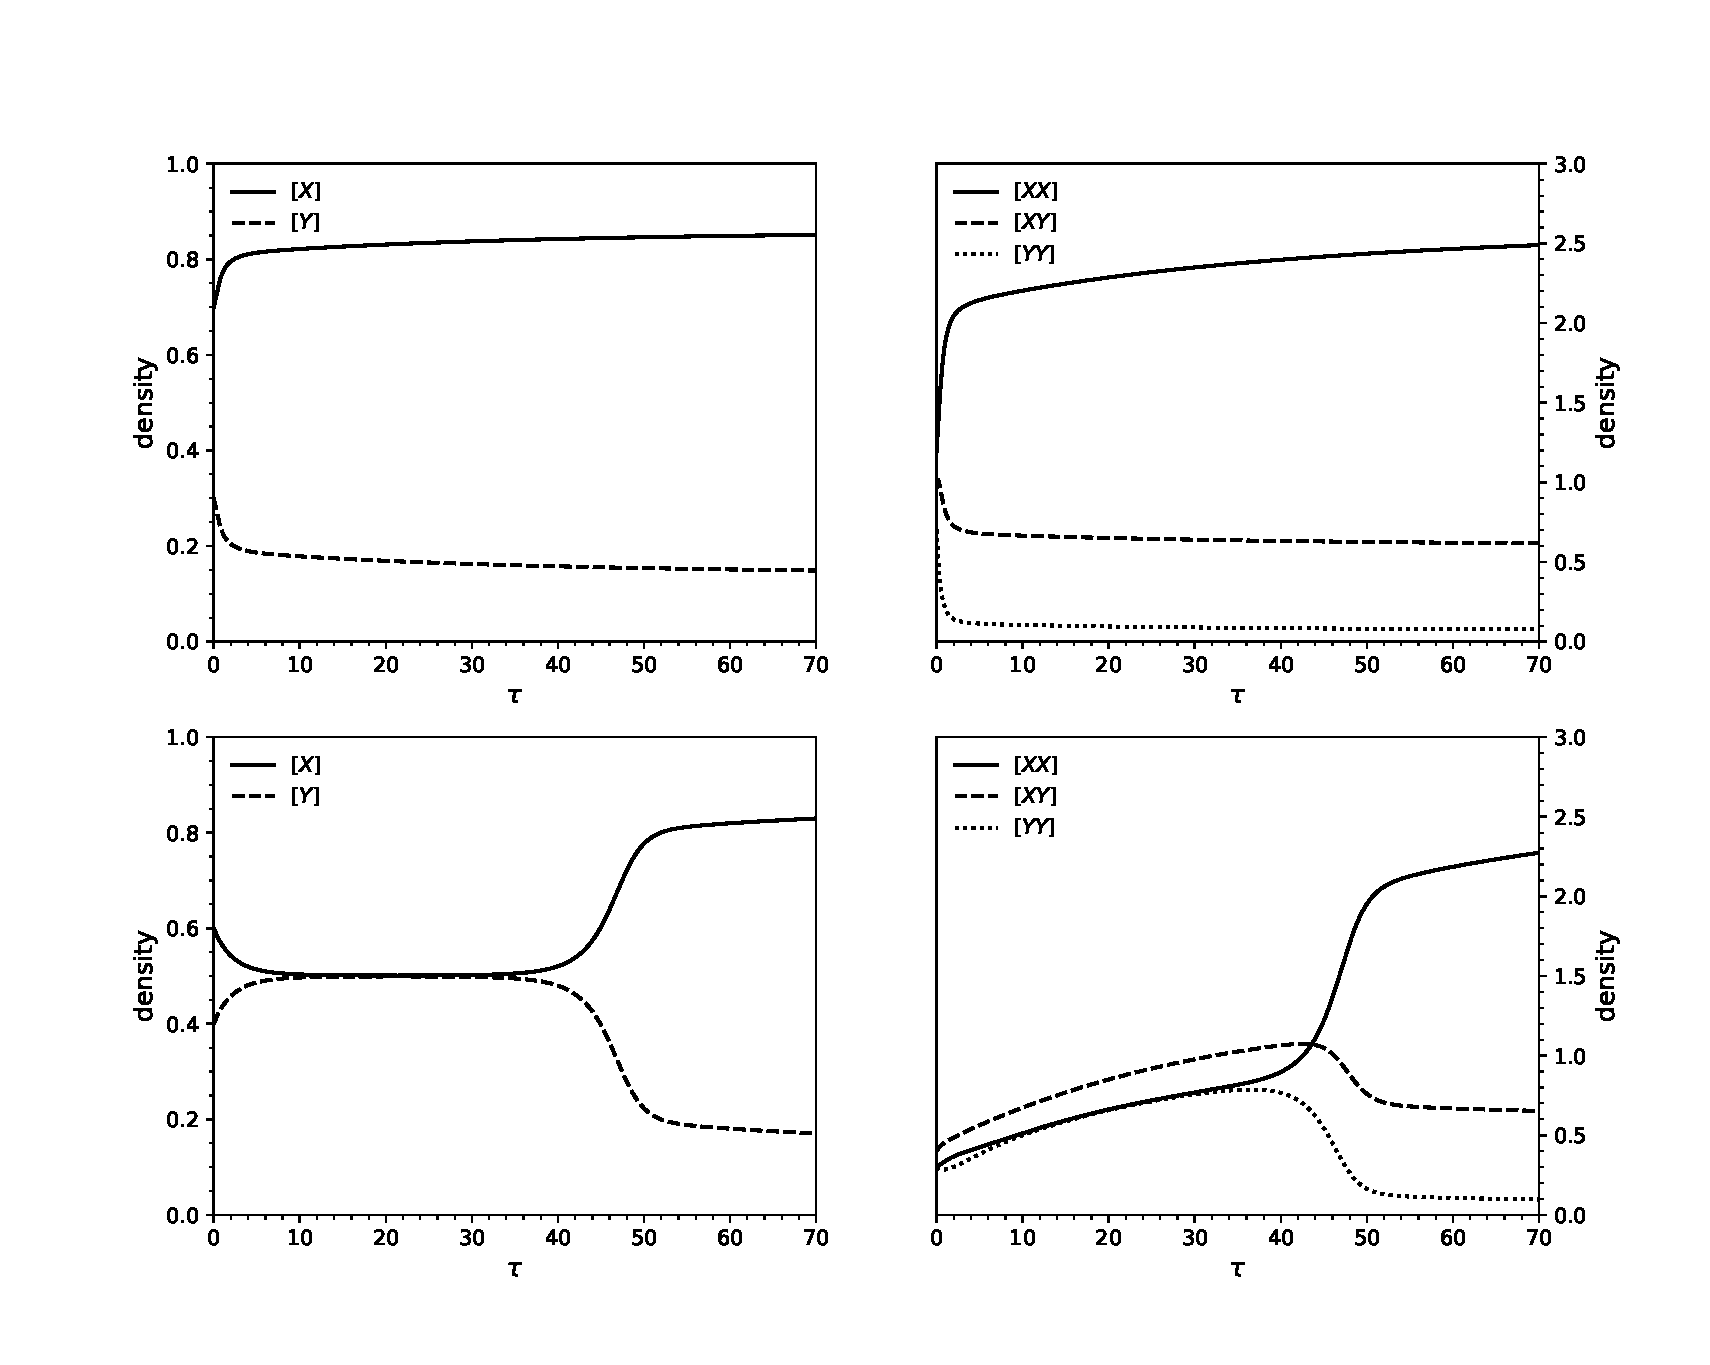
\includegraphics[width = 0.85\textwidth, trim={0 0.5cm 0 2cm},clip=true]{figures/discrete_double_run_1} %trim crops the image on the top such that it fits nicely on the page, trim is activated by option clip=true
		\caption{$\eta = 0.3, \sigma_d = 0.2, \alpha = 0.5, \beta = 0.1$}
		\label{fig:typical_behaviour1}
	\end{subfigure}
	\begin{subfigure}{\textwidth}
		\centering
		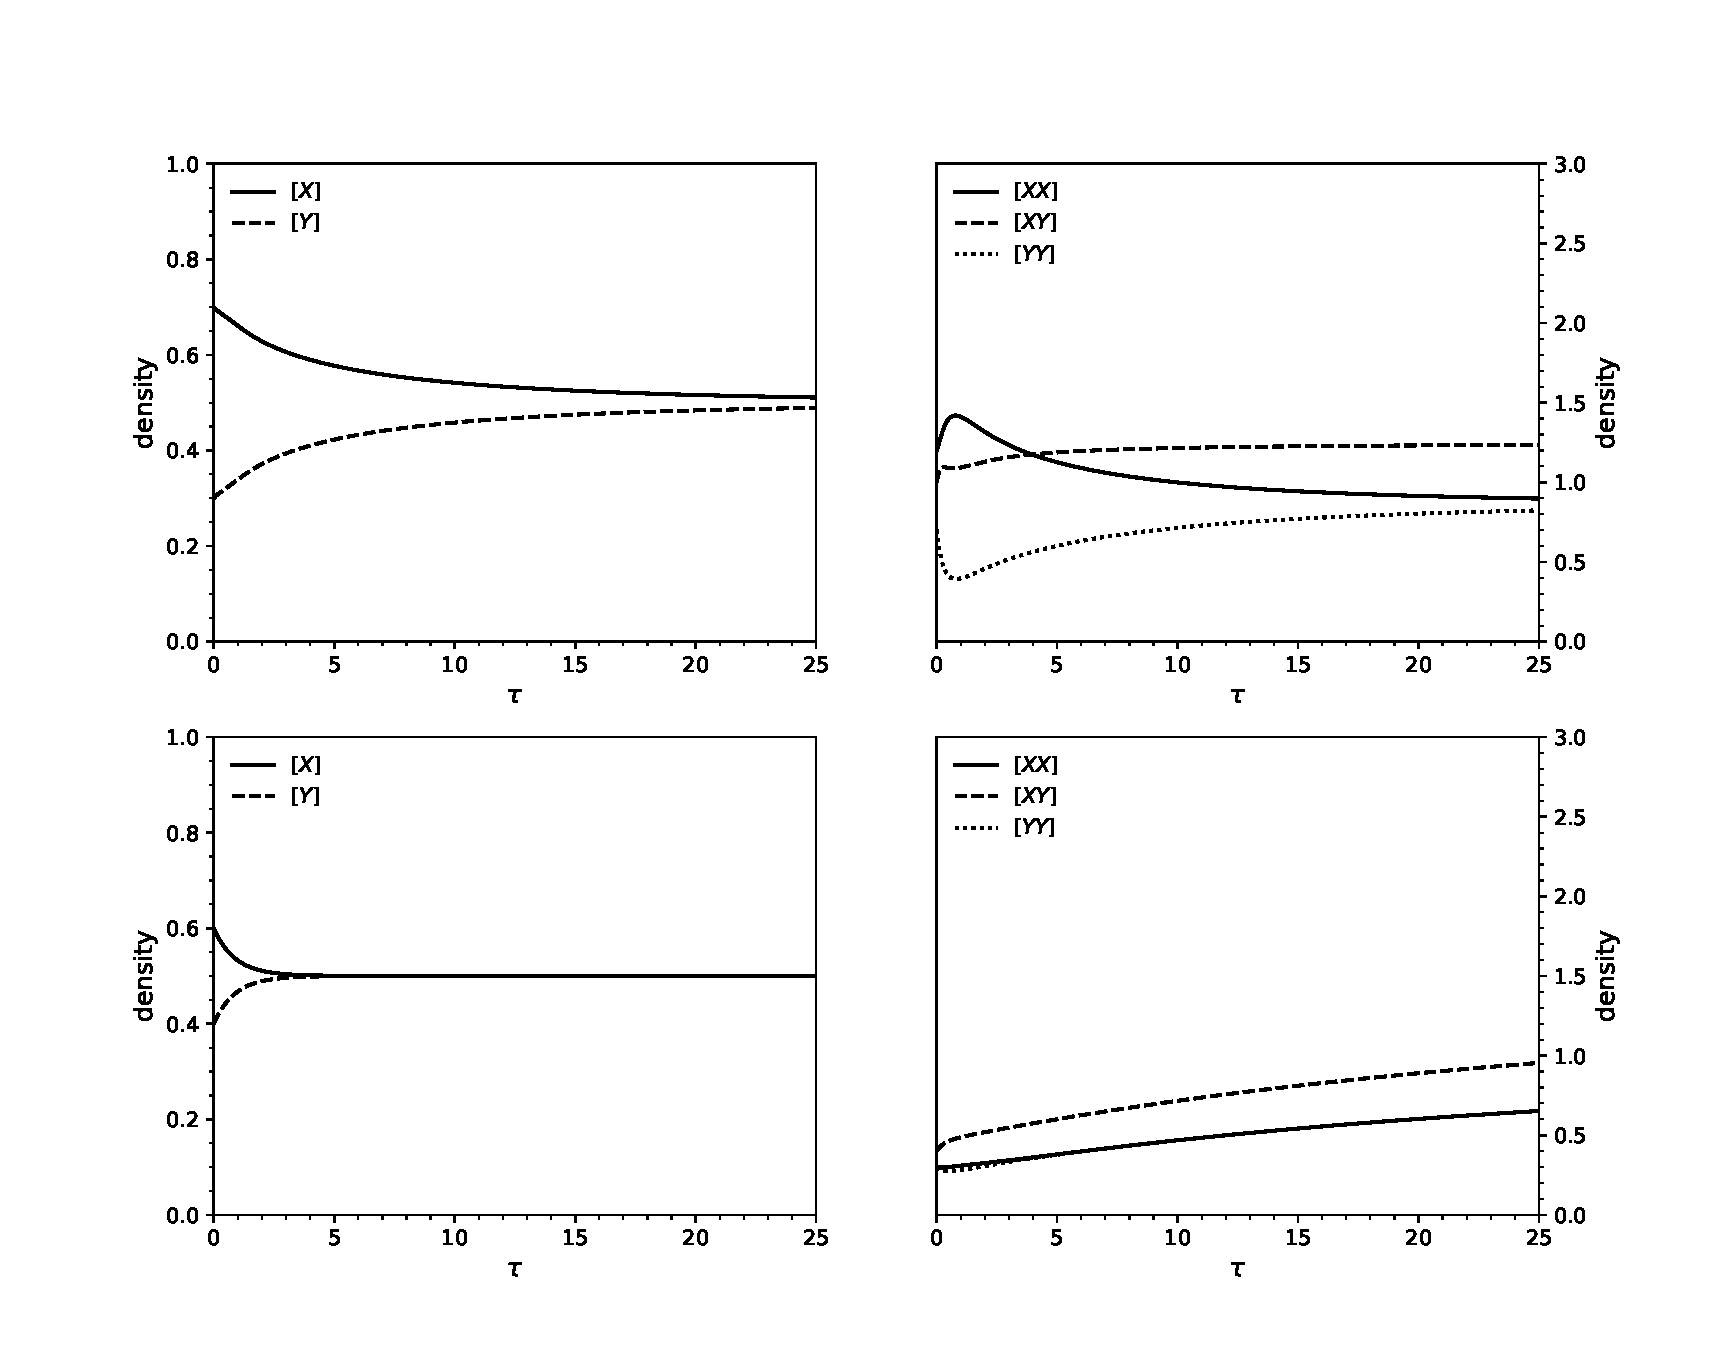
\includegraphics[width = 0.85\textwidth, trim={0 0.5cm 0 1cm},clip=true]{figures/discrete_double_run_2}
		\caption{$\eta = 0.65, \sigma_d = 0.2, \alpha = 0.5, \beta = 0.1$}
		\label{fig:typical_behaviour2}
	\end{subfigure}
	\caption{Behaviour of the two-state adaptive network model for different system parameters and initial conditions. All six figures graph the density of the zeroth moments (left) and the first moments (right) versus the discrete time index $\tau$. In both figure (a) and (b) the initial conditions were taken as $\X=0.7, \Y=0.3, \XX=1.2, \YY=0.7$ $\XY=1.0$ for the upper set of graphs and as $\X=0.6, \Y=0.4, \XX=0.3, \YY=0.3$ $\XY=0.4$ for the lower set. Figures (a) and (b) differ in system parameters $\eta, \sigma_d, \alpha$ and $\beta$.}
%moments1 = [0.7, 0.3, 1.2, 1.0, 0.7]
%moments2 = [0.6, 0.4, 0.3, 0.4, 0.3]
	\label{fig:typical_behaviour}
\end{figure}

In \cref{fig:typical_behaviour2}, the system parameters are chosen such that the system converges to a different stationary solution. This solution is called the \textit{disordered} stationary solution since all states are equally distributed over all nodes. Hence, we have $[\omega] = \frac{1}{M}$ for all $\omega\in\Omega$. In this case, we see that convergence occurs relatively slow if the initial link densities are chosen high, compared to the case where they are lower. Moreover, when the network converges to the disordered solution, it seems that the homogeneous link densities $\XX$ and $\YY$ converge to the same value.

The four different cases in the figure give a good insight into how the system behaves under different conditions. In the next section, we will perform a bifurcation analysis to gain quantitative knowledge of under what conditions the system may and up in what final state.

\section{Bifurcation analysis of the 2-state adaptive network model}

In the previous section, we gained some insight into the behaviour of the two-state adaptive network model. In some cases, the state densities converged to the disordered solution $\X~=~\Y~=~\frac{1}{2}$, while for other system parameters the distributions got very close to the disordered distribution before they converged to their true fixed point.  This behaviour suggests that the disordered solution is either a stable node or a saddle point. In the case of a saddle point, the densities in the unstable manifold might approach the saddle point very slowly before they suddenly shoot away to the final ordered solution. This would also explain the convergence rates. In order to check if this is the case, we will analyse the linear stability in $\X~=~\Y~=~\frac{1}{2}$. 

The two state adaptive network model in \cref{eq:M2system_closure_written_out} can be rewritten as 
\begin{equation}
\bm{\dot{x}} = \bm{f}(\bm{x}),
\end{equation}
for
\begin{equation*}
\bm{x} =
\begin{bmatrix}
\X\\
\Y\\
\XX\\
\YY\\
\XY
\end{bmatrix} 
\hspace{10mm}
\text{and}
\hspace{10mm}
\bm{f}(\bm{x}) = 
\begin{bmatrix}
f_1(\bm{x})\\
f_2(\bm{x})\\
f_3(\bm{x})\\
f_4(\bm{x})\\
f_5(\bm{x})
\end{bmatrix} 
\end{equation*}
where Newton's dot notation is used to indicate the derivative with respect to time $t$. For a solution $\bm{x}^*$ to be a stationary solution (also fixed point, steady state solution or equilibrium solution) we have $\bm{f}(\bm{x}^*)=\bm{0}$ by definition \cite{Strogatz1994}.

%%%%%%%%%%%%%%%%%%%%%%%%%%%%%%%%%%%%%%%%%%%%%%%%%%%%%%%%%%%%%%%%%%%%%%%%%%%%%%%%%%%%%%%%%%%%%

\subsection{Finding fixed points}

In order to obtain expressions for the fixed points of the system, we will be solving $\bm{f}(\bm{x}^*)=\bm{0}$. Therefore, all time derivatives are equated to zero. We start with setting $\frac{d}{dt}\X =0$ or $\frac{d}{dt}\Y=0$, which yields $\X=\Y$ or $\X\Y=\frac{\sigma_d \XY^2}{2\eta}$. Imposing the conservation law $\X+\Y=1$ on the first solution gives $\X=\Y=\frac{1}{2}$. Equating the other time derivatives to zero should give the other coordinates of the fixed point. If we first solve $\frac{d}{dt}\XX= \frac{d}{dt}\YY=0$ we obtain two results, one of which is
\begin{equation}    
\XX=\YY = \frac{\alpha}{8\beta}\frac{ \sigma_d \alpha^2 +4\sigma_d \alpha \beta + 8\eta \beta^2 }{\sigma_d \alpha^2+8\eta \beta^2} = \frac{l}{8}\frac{l^2+4l+8s}{l^2+8s},
\end{equation}
in which we define $l=\frac{\alpha}{\beta}$ as the dimensionless link creation ratio and $s=\frac{\eta}{\sigma_d}$ as the dimensionless noise ratio. 
The other solution is $\eta = 0 \land \left( \sigma_d =0 \lor \XY=0 \right)$. This corresponds to either a network with only link dynamics, implying all node states stay unchanged, or to a network with no flipping noise and no heterogeneous $XY$-links. In the latter case the network is either disconnected or homogeneous such that all nodes are in the same state. Since $\X=\Y=\frac{1}{2}$ and we assume the network is connected this solution can be safely considered as a trivial solution and therefore be omitted. 
Lastly setting $\frac{d}{dt}\XY=0$ gives 
\begin{equation}
\XY = \frac{\alpha}{4\beta} =\frac{l}{4}.
\end{equation}
Combined, the first set of fixed points $\bm{x}^*_1$ is given by 
\begin{equation}
\bm{x}^*_1 = 
\begin{bmatrix}
\frac{1}{2}\\[1ex]
\frac{1}{2}\\[1ex]
\frac{l}{8}\frac{l^2+4l+8s}{l^2+8s}\\[1ex]
\frac{l}{8}\frac{l^2+4l+8s}{l^2+8s}\\[1ex]
\frac{l}{4}
\end{bmatrix},
\end{equation}
corresponding to the disordered stationary solutions. 

We can analyse the stability of the other branch $\X,\Y \neq \frac{1}{2}$ in the same manner. Here we already found $\X\Y=\frac{\sigma_d \XY^2}{2\eta}$. Using the other ODEs, the resulting second set of fixed points $\bm{x}^*_2$ is given as
\begin{equation}
\bm{x}^*_2 = 
\begin{bmatrix}
\frac{1}{2} \pm \frac{1}{2} \sqrt{1-8 \frac{s}{l^2}}\\[1ex]
\frac{1}{2} \mp \frac{1}{2} \sqrt{1-8 \frac{s}{l^2}}\\[1ex]
\frac{s}{l} \left( 1+ \frac{2}{l} \right) \frac{1 \pm \sqrt{1-8\frac{s}{l^2}}}{1 \mp \sqrt{1-8\frac{s}{l^2}}}\\[1ex]
\frac{s}{l} \left( 1+ \frac{2}{l} \right) \frac{1 \mp \sqrt{1-8\frac{s}{l^2}}}{1 \pm \sqrt{1-8\frac{s}{l^2}}}\\[1ex]
\frac{2s}{l}
\end{bmatrix},
\end{equation}
which corresponds to the ordered state solutions. It turns out that the exact density of states $X$ and $Y$ depend on the two system parameters $s$ and $l$ only. Which of the two has the highest density depends on the initial condition; the one with the highest initial density will have the highest stationary state density. 

The fixed points densities are plotted against $s$ for various values of $l$ in the bifurcation diagrams in \cref{fig:bifurcation_zerothM} and \cref{fig:bifurcation_firstM} on the left hand side, whilst they are plotted versus $l$ for various values of $s$ on the right hand side. In \cref{fig:bifurcation_zerothM} we see that for a high noise ratio $s$, the system will converge to a disordered state, while if the noise rate drops below a certain value (depending on $l$), two extra ordered solutions emerge. For low link creation rates $l$ the system also converges to a disordered solution. If $l$ is increased then there is a critical value (depending on $s$) where the same two ordered solutions are formed. From \cref{fig:bifurcation_firstM} we deduce that $l$ determines the density of $XY$-links in the system and that if $l$ is increased, then the overall total number of links increases. On the other hand, higher values of $s$ cause a lower overall link density. If the system converges to an ordered solution, then there are relatively many homogeneous links corresponding to the highest density state, hence, all nodes in the same state will be highly connected. Finally, if the system converges to the ordered state the number of $XY$-links depends linearly on the rate $s$, but if it converges to a disordered state it depends linearly on the rate $l$. 


Finally we note that these fixed points are consistent with the assumption $\alpha\X\Y = \beta\XY$ on both branches, which was made in \cite{Chen2016} to simplify the system in order to allow for analytical evaluation.

\begin{figure}[htp]
	\centering
	\makebox[\textwidth][c]{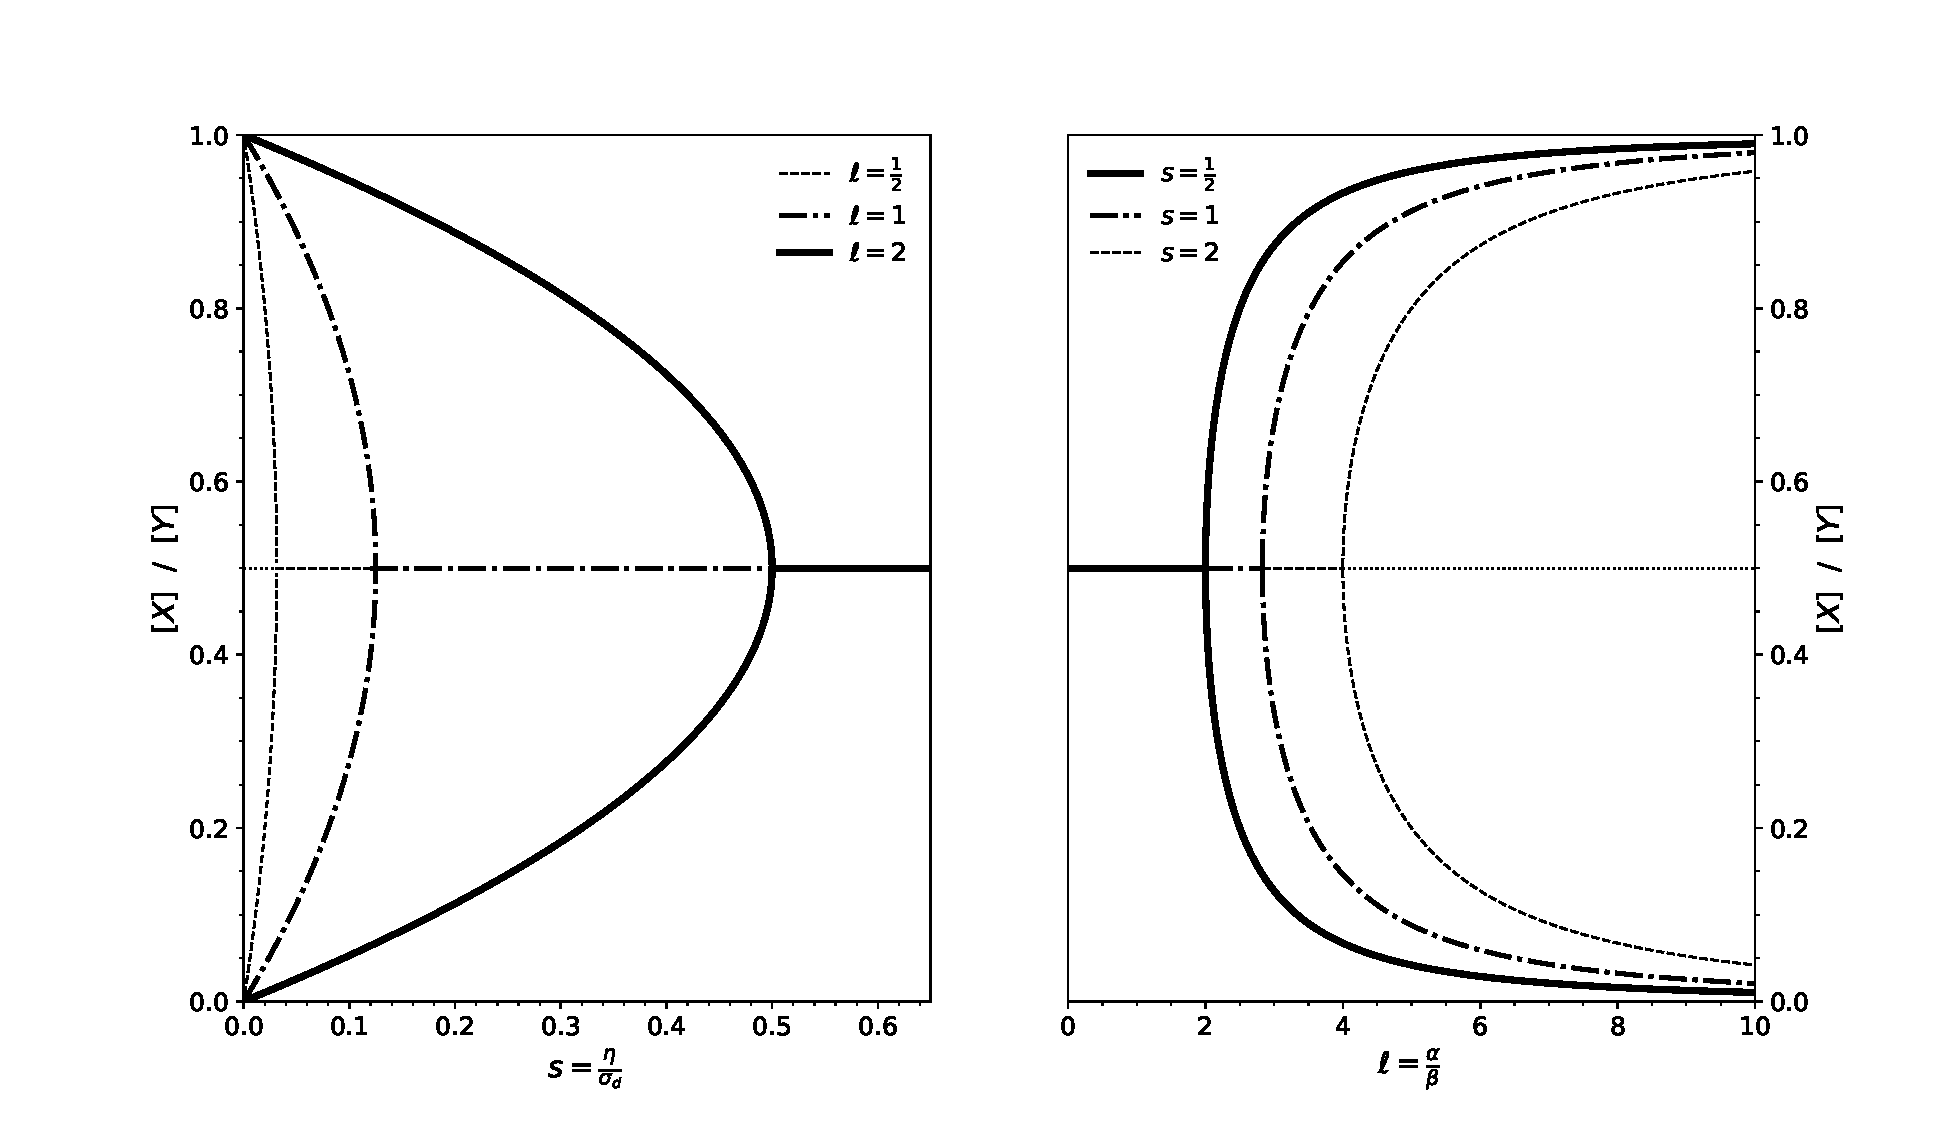
\includegraphics[width = 1.1\textwidth]{figures/bifurcation_zeroth}}
	\caption{Bifurcation diagrams of the two state adaptive network model. The ordered and disordered stationary solutions of state densities $\X, \Y$ for various values of the link creation parameter $l$ as function of the noise ratio $s$ (left) and for various values of $s$ as function of $l$ (right). Both stable and unstable solutions are plotted. The bifurcation is a supercritical pitchfork bifurcation.}
	\label{fig:bifurcation_zerothM}
\end{figure}
\begin{figure}[htp]
	\centering
	\begin{subfigure}{\textwidth}
		\centering
		\makebox[\textwidth][c]{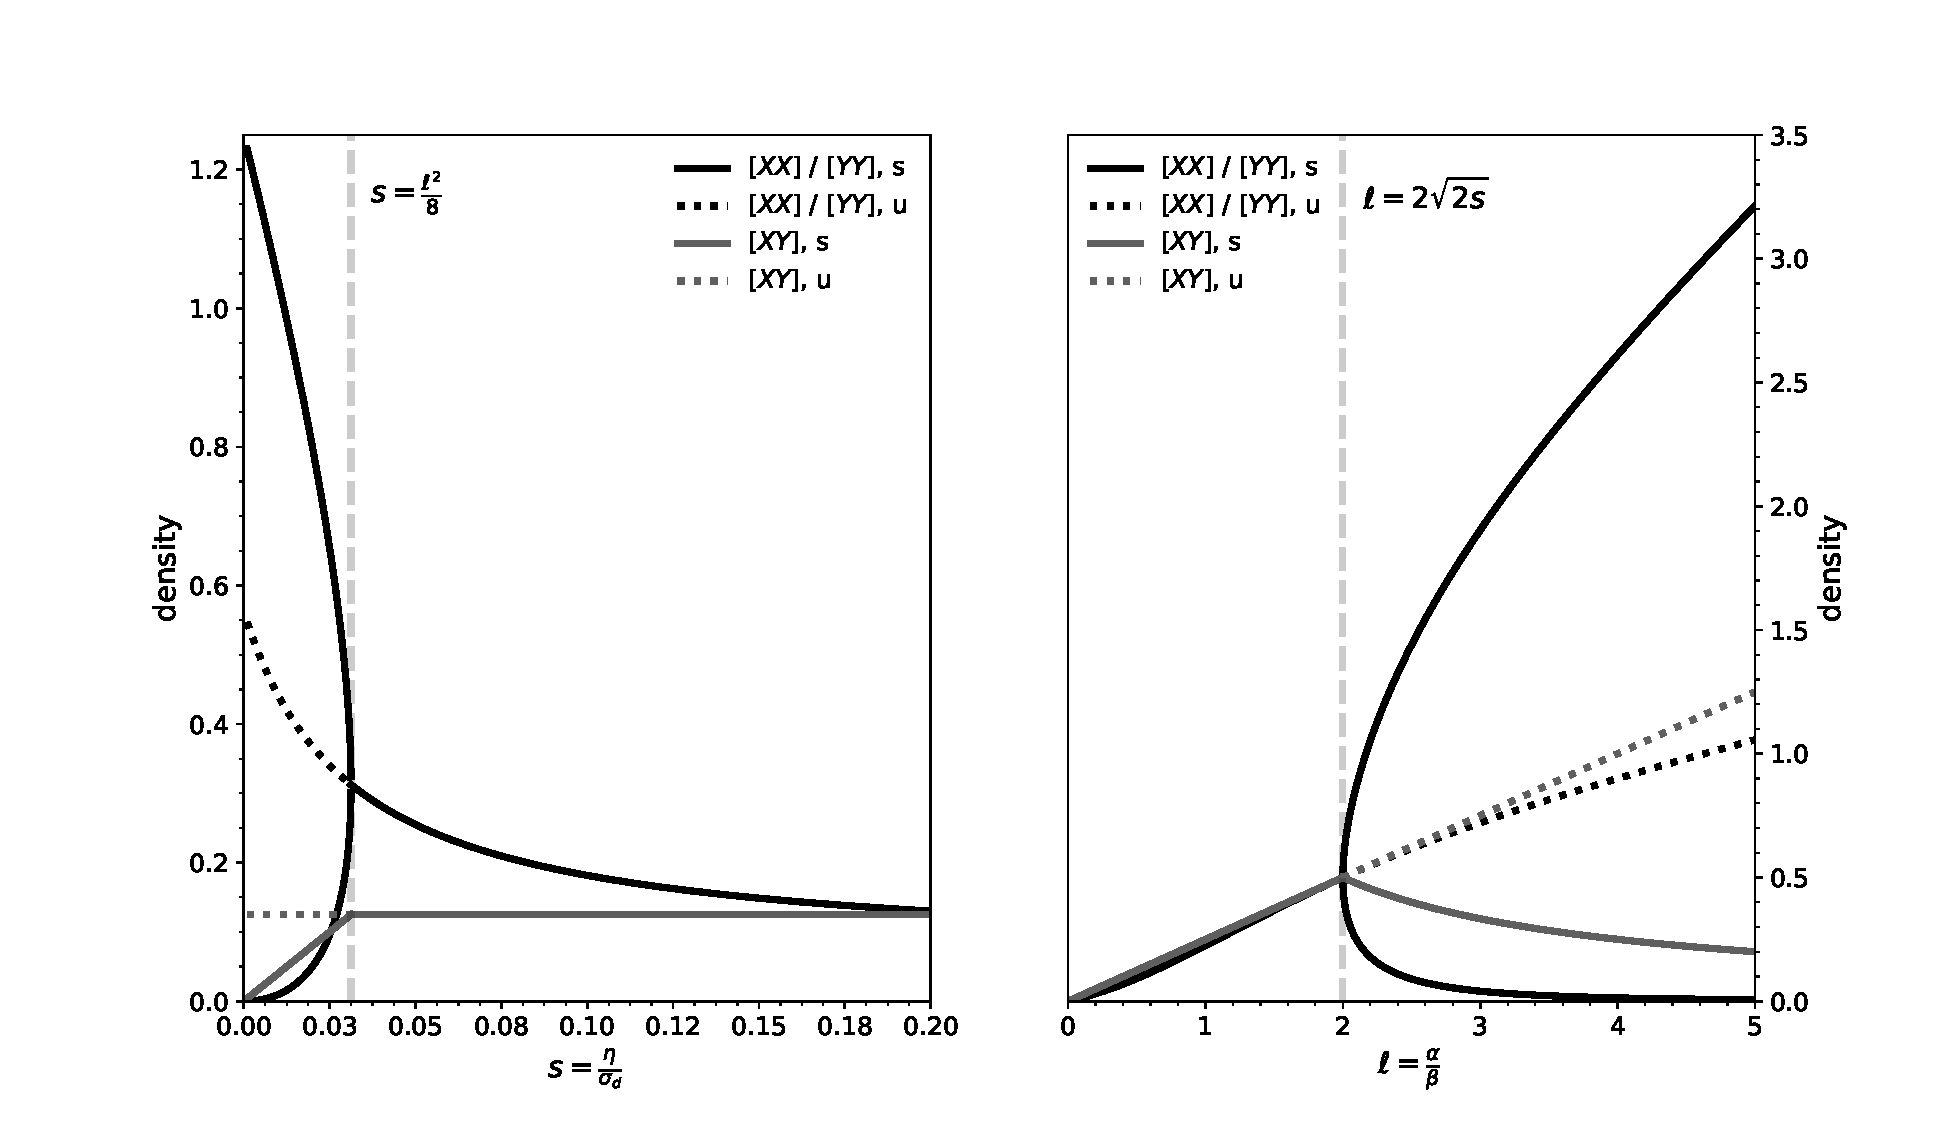
\includegraphics[width = 1.1\textwidth, trim={0 0cm 0 0cm},clip=true]{figures/bifurcation_first_s_05_l_05_BW}}% %trim crops the image on the top such that it fits nicely on the page, trim is activated by option clip=true
		\caption{\qquad\qquad $l=\frac{1}{2}$ \hspace{4.8cm} $s=\frac{1}{2}$ \qquad\qquad\quad}
		\label{}
	\end{subfigure}
	\begin{subfigure}{\textwidth}
		\centering
		\makebox[\textwidth][c]{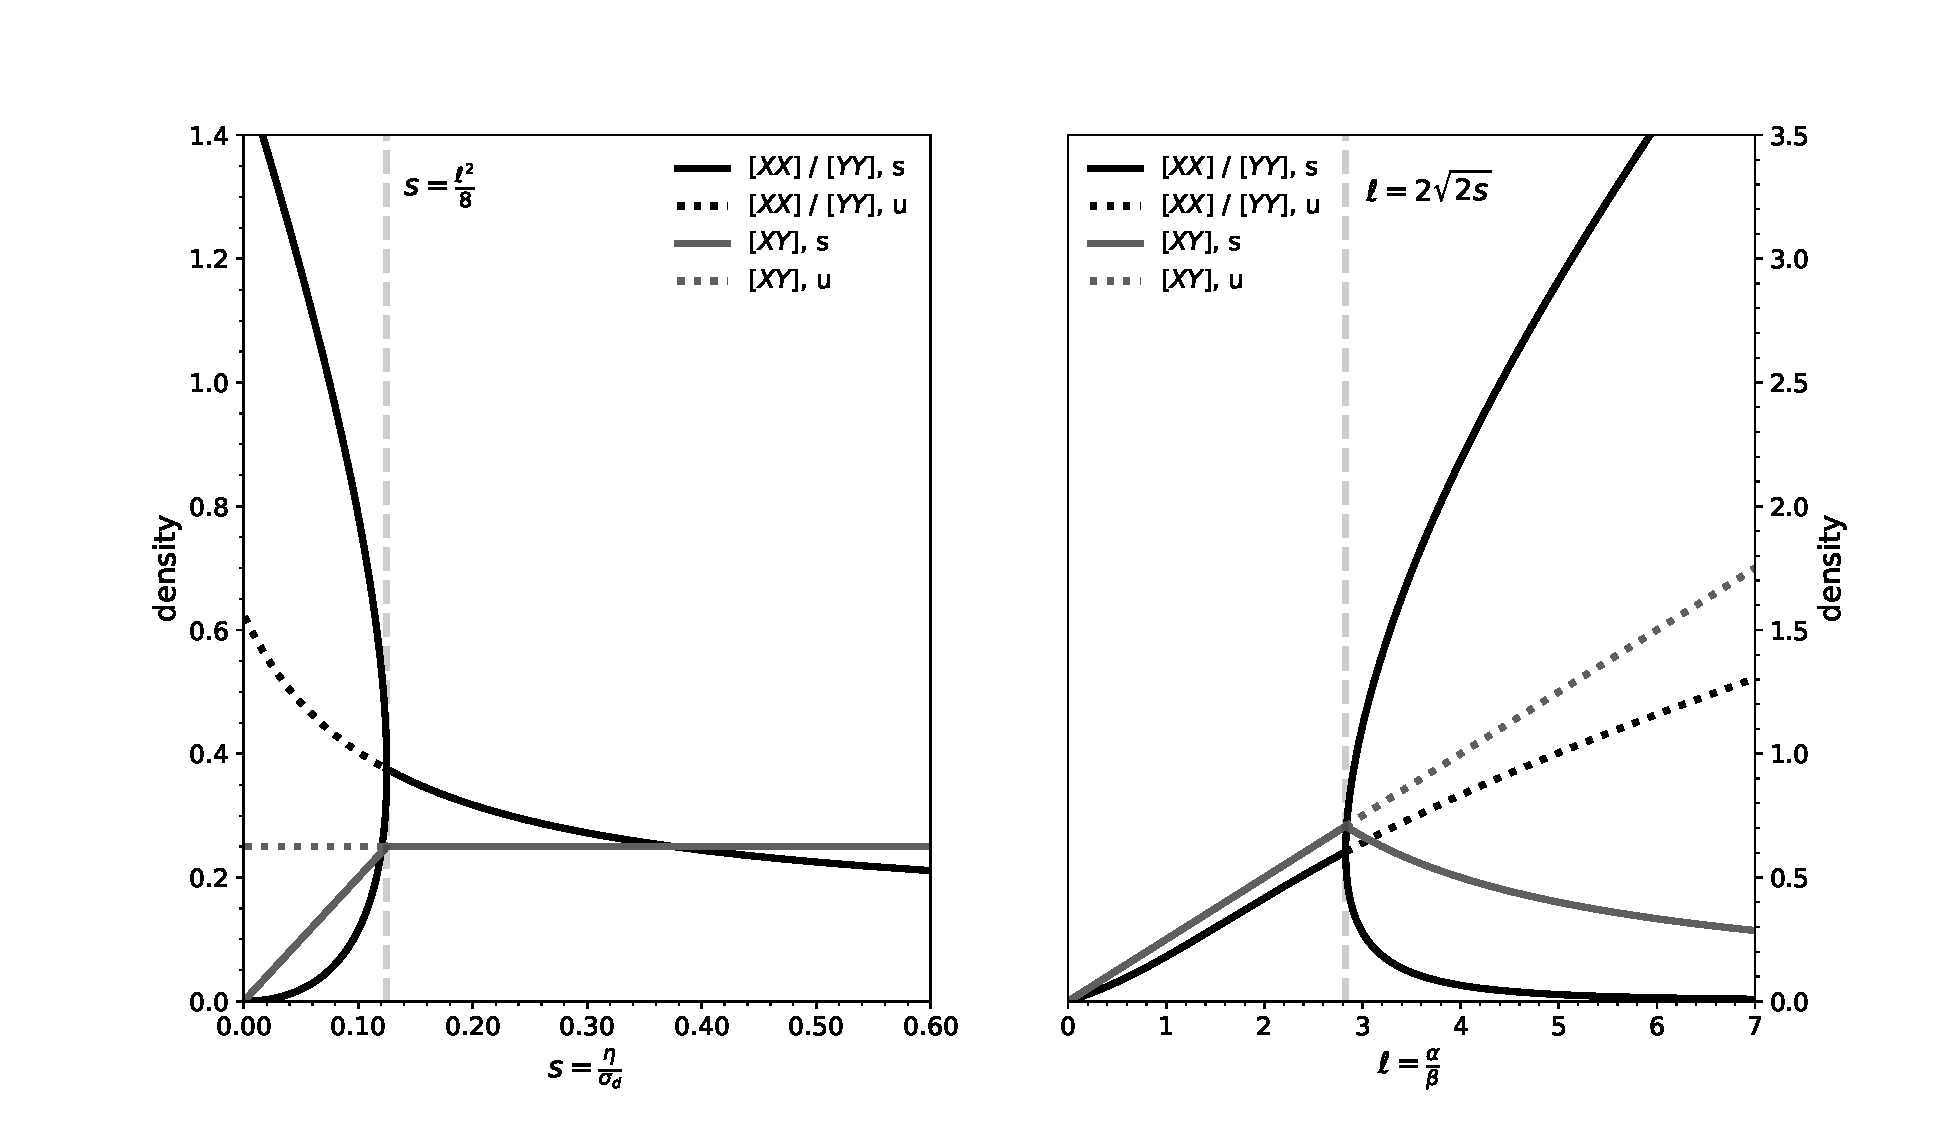
\includegraphics[width = 1.1\textwidth, trim={0 0cm 0 0cm},clip=true]{figures/bifurcation_first_s_1_l_1_BW}}
		\caption{\qquad\qquad $l=1$ \hspace{4.8cm} $s=1$ \qquad\qquad\quad}
		\label{}
	\end{subfigure}
	\caption{(continues on next page)}
\end{figure}
\clearpage
\begin{figure}[htp]
	\ContinuedFloat
	\begin{subfigure}{\textwidth}
		\centering
		\makebox[\textwidth][c]{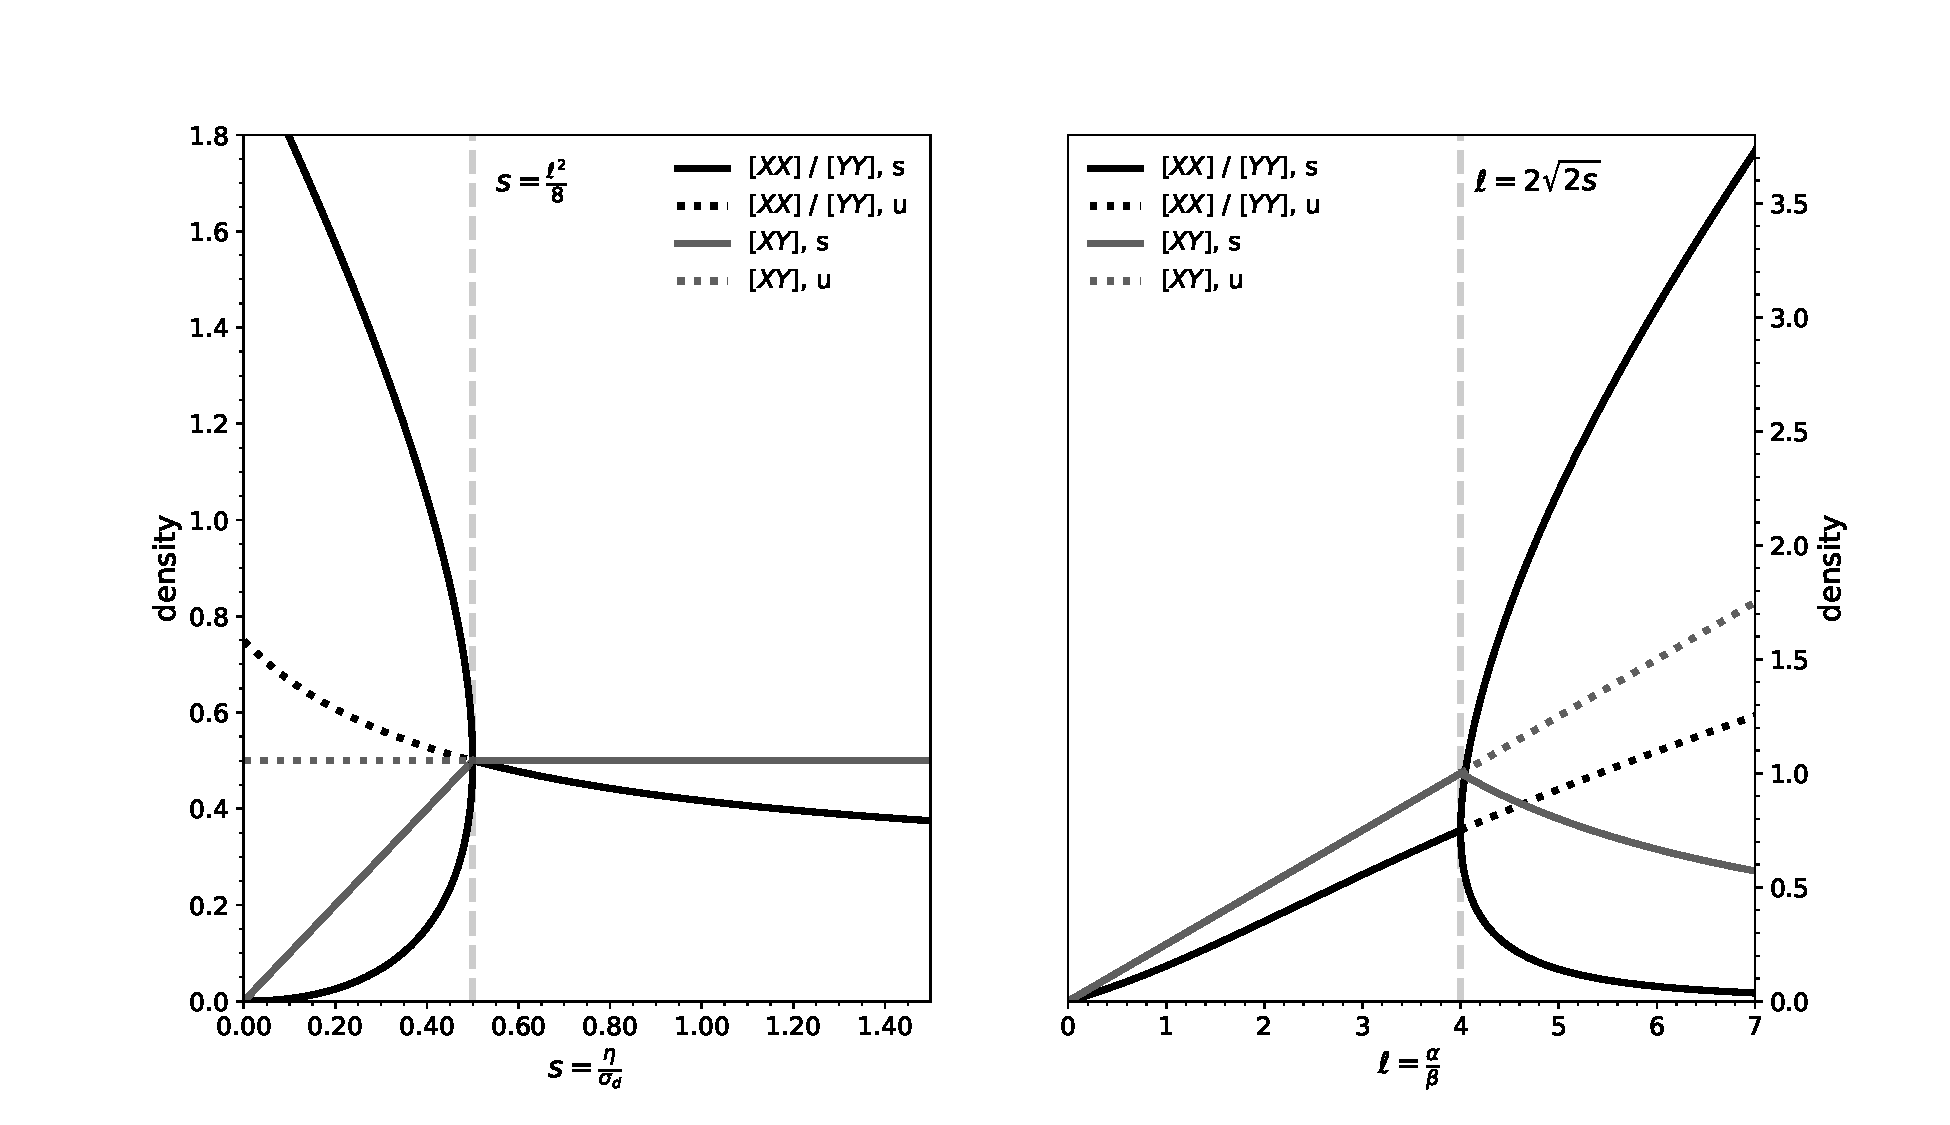
\includegraphics[width = 1.1\textwidth, trim={0 0cm 0 0cm},clip=true]{figures/bifurcation_first_s_2_l_2_BW}}
		\caption{\qquad\qquad $l=2$ \hspace{4.8cm} $s=2$ \qquad\qquad\quad}
		\label{}
	\end{subfigure}
	\caption{Bifurcation diagrams of the two state adaptive network model. (left) The stationary solutions of link densities $\XX, \YY, \XY$ for various values of the link creation parameter $l$ as function of the noise ratio $s$. The stable disordered stationary solutions are on the right hand side of the line $s=\frac{l^2}{8}$, while the unstable disordered solutions are on the left hand side plotted with a dotted line. The bold curves on the left hand side indicate the ordered stationary solutions. (right) The stationary solutions of link densities $\XX, \YY, \XY$ for various values of $s$ as function of $l$. The stable disordered stationary solutions are on the left hand side from the line $l=2\sqrt{2s}$, while the unstable disordered solutions are on the right hand side plotted with a dotted line. The bold curves on the right hand side indicate ordered stationary solutions. Note that the axis scales differ. }
	\label{fig:bifurcation_firstM}
\end{figure}

\subsection{Linearisation}
For further stability analysis, we will proceed with a linearisation of the system of ODEs around its fixed points $\bm{x}^*$. This can be done as follows
\begin{equation}
\begin{aligned}
\bm{f}(\bm{x}^* + \Delta \bm{x}) 
&= \bm{f}( \bm{x}^* ) + J\rvert_{ \bm{x}^* }  \Delta \bm{x}  + \mathcal{O}(\Vert \Delta \bm{x} \Vert^2_2)\\
&\approx J\rvert_{ \bm{x}^* }  \Delta \bm{x},
\end{aligned}
\end{equation} 
in which the Jacobian matrix $J$ is defined component-wise by $J_{i,j} = \frac{\partial f_i}{\partial x_j}$ with $x_j$ an element of $\bm{x}$.
Now in order to evaluate the stability of the found fixed points, we will need the theorem of Lyapunov, which enables us to find the stability by evaluation of the eigenvalues of the Jacobian matrix. The proof is not written out here, since it can be found in various books on basic differential equation or bifurcation theory, for example \cite{Boyce2010, Braun1993}.

\begin{theorem}[Lyapunov]
	Let $f: \mathbb{R}^n \to \mathbb{R}^n$ be an element of $C^1$ and $\bm{x}^*$ be a fixed point of $\bm{\dot{x}} = \bm{f}(\bm{x})$. Let $\bm{\dot{x}} = J\rvert_{ \bm{x}^* }  \bm{x}$ be the linearization of $f$ with $J$ the Jacobian matrix with eigenvalues $\lambda_1,..,\lambda_n$. $\bm{x}^*$ is
	\begin{enumerate}
		\item asymptotically stable if $\Re \lambda_i < 0$ for all $i \in \{1,...,n\}$,
		\item unstable if $\Re \lambda_i > 0$ for some $i \in \{1,...,n\}$
	\end{enumerate}
\end{theorem}
Note that the theorem does not say anything if $\Re \lambda_i = 0$ for some $i \in \{1,...,n\}$. Hence, further analysis is necessary in that case. This theorem is applicable since $\bm{f}$ is continuous in time $t$. Using Maple 2018 the Jacobian matrix is evaluated in the first set of fixed points $\bm{x}^*_1$. The resulting five eigenvalues can be written as
\begin{subequations}
	\label{eq:eigenvalues}
	\begin{alignat}{3}
	\lambda_1 &= 0& \\
	\lambda_2 &= 
	\frac{\phantom{-} \sigma_d \alpha^2 - 8\eta \beta^2}{4\beta^2} 
	&& = \phantom{-} \frac{1}{4}\sigma_d l^2 -2\eta\\  %phantom is used to align the fractions. it replaces the exact space the minus sign takes with white space
	\lambda_3 &= 
	\frac{- \sigma_d \alpha^2 - 8\eta \beta^2}{4\beta^2} 
	&& = -\frac{1}{4}\sigma_d l^2 -2\eta\\
	\lambda_4 &= \frac{\phantom{-}\sqrt{b^2-4ac}-b}{2a} & \\
	\lambda_5 &= \frac{-\sqrt{b^2-4ac}-b}{2a},  &
	\end{alignat}
\end{subequations}
where the latter two eigenvalues are written in terms of a certain $a, b, c \in \mathbb{R}_{>0}$, which are quite elaborate expressions in terms of parameters $\eta, \sigma_d, \alpha$ and $\beta$.  

According to the theorem, each eigenvalue with negative real part corresponds to an asymptotically stable manifold of the fixed point $\bm{x}^*_1$ in the phase plane, whilst each eigenvalue with positive real part will have an eigenvector corresponding to an unstable manifold. Before evaluating these eigenvalues, note that $\lambda_1$ is a zero eigenvalue, which emerges because the conservation law $\X+\Y=1$ is imposed on the system. In fact, this directly implies that there only exist valid solutions to the system of ODEs in a four-dimensional subspace of the five-dimensional $\left( \X, \Y, \XX, \YY, \XY \right)$ space. These statements are formalized in the following theorem. 

\begin{theorem}
	\label{th:conservation_implies_zero_eigenvalue}
	If a conservation law is imposed on a system of first order ODEs, then the corresponding Jacobian matrix $J$ has at least one eigenvalue zero.
\end{theorem}
\begin{proof}
	Let $\dot{\bm{x}} = \bm{f}(\bm{x})$ be a system of first order ODEs in which $\bm{x} = [x_1, x_2, ..., x_n]^T$ and $\bm{f(x)} = [f_1(\bm{x}), f_2(\bm{x}), ..., f_n(\bm{x})]^T$. Furthermore suppose there is a conservation law, which means that a certain linear combination of time derivatives equals zero. This law enables us to express one derivative in terms of the other derivatives. Assume without loss of generality  $\dot{x_1}=h(\dot{x}_2,...,\dot{x}_n)$, with $h$ a linear function. Using the system of equations we then find $f_1(\bm{x}) = \dot{x_1}=h(\dot{x}_2,...,\dot{x}_n) = h(f_2(\bm{x}), ..., f_n(\bm{x}))$.
	
	The Jacobian matrix $J$ is defined as
	\begin{equation*}
	\begin{aligned}
	J = \frac{\partial (f_1,...,f_n)}{\partial (x_1,...,x_n)}
	&=  
	\begin{bmatrix}
	\frac{\partial f_1}{\partial x_1} &
	\frac{\partial f_1}{\partial x_2} &
	\dots & 
	\frac{\partial f_1}{\partial x_n} \\[1ex] % <-- 1ex more space between    rows of matrix
	\frac{\partial f_2}{\partial x_1} &
	\frac{\partial f_2}{\partial x_2} &
	\dots & 
	\frac{\partial f_2}{\partial x_n} \\[1ex] % <-- 1ex more space between    rows of matrix
	\vdots & 
	\vdots &
	\ddots & 
	\vdots \\[1ex]
	\frac{\partial f_n}{\partial x_1} &
	\frac{\partial f_n}{\partial x_2} &
	\dots & 
	\frac{\partial f_n}{\partial x_n}
	\end{bmatrix}\\[1ex]
	&=  
	\begin{bmatrix}
	\frac{\partial h(f_2(\bm{x}), ..., f_n(\bm{x}))}{\partial x_1} &
	\frac{\partial h(f_2(\bm{x}), ..., f_n(\bm{x}))}{\partial x_2} &
	\dots & 
	\frac{\partial h(f_2(\bm{x}), ..., f_n(\bm{x}))}{\partial x_n} \\[1ex] % <-- 1ex more space between    rows of matrix
	\frac{\partial f_2}{\partial x_1} &
	\frac{\partial f_2}{\partial x_2} &
	\dots & 
	\frac{\partial f_2}{\partial x_n} \\[1ex] % <-- 1ex more space between    rows of matrix
	\vdots & 
	\vdots &
	\ddots & 
	\vdots \\[1ex]
	\frac{\partial f_n}{\partial x_1} &
	\frac{\partial f_n}{\partial x_2} &
	\dots & 
	\frac{\partial f_n}{\partial x_n}
	\end{bmatrix}\\[1ex]
	&=  
	\begin{bmatrix}
	h\left( \frac{\partial f_2}{x_1},...,\frac{\partial f_n}{x_1} \right) &
	h\left( \frac{\partial f_2}{x_2},...,\frac{\partial f_n}{x_2} \right) &
	\dots & 
	h\left( \frac{\partial f_2}{x_n},...,\frac{\partial f_n}{x_n} \right) \\[1ex] % <-- 1ex more space between    rows of matrix
	\frac{\partial f_2}{\partial x_1} &
	\frac{\partial f_2}{\partial x_2} &
	\dots & 
	\frac{\partial f_2}{\partial x_n} \\[1ex] % <-- 1ex more space between    rows of matrix
	\vdots & 
	\vdots &
	\ddots & 
	\vdots \\[1ex]
	\frac{\partial f_n}{\partial x_1} &
	\frac{\partial f_n}{\partial x_2} &
	\dots & 
	\frac{\partial f_n}{\partial x_n}
	\end{bmatrix}.
	\end{aligned}
	\end{equation*}
	Since $h$ is a linear function, it is possible to find a matrix $A$ which defines row operations such that $A J $ has a row containing only zeros. This implies $\det(AJ) = 0 = \det(AJ-\lambda I)$ for $\lambda=0$. Therefore $AJ$ has an eigenvalue $\lambda=0$. It follows directly that the Jacobian matrix $J$ also has an eigenvalue $\lambda=0$, since row operations leave the eigenvalues unchanged.
\end{proof}

Because the Jacobian matrix has one row which is linearly dependent on the other rows, $\text{rank}( J) \leq n-1$. This means that the solutions to the system are all found on a subspace of maximum dimension $n-1$ of the phase space. This also means that the system can be reduced to an identical four-dimensional system, in which the zero eigenvalue disappears. Therefore $\lambda_1=0$ does not influence the stability. 

Looking at the other eigenvalues, we see that $\lambda_2$ and $\lambda_3$ differ by a minus sign. Demanding $\lambda_2 < 0$ gives 
\begin{equation}
l^2<8s,
\end{equation}
as a condition for asymptotic stability of $\bm{x}_1^*$. Furthermore, since $\eta, \sigma_d, \alpha, \beta > 0$ we have $\lambda_3 < 0$. The last two eigenvalues $\lambda_4$ and $\lambda_5$ also differ by a minus sign. Using Maple, it was verified that $0 < 4ac < b^2$, which implies $\sqrt{b^2-4ac}  < b$. Since $2a > 0$ we have $\lambda_4 < 0$. Also using the fact that $a, b, c > 0$ it can be concluded that $ \lambda_5 < 0$.

Altogether, $\lambda_1$ does not influence the stability, $\lambda_2$ demands $l^2 < 8s$ for a stable manifold in the phase plane and $\lambda_3, \lambda_4, \lambda_5 < 0$ create stable manifolds in all cases. This makes $\bm{x}^*_1$ a stable node in phase space for $l^2 < 8s$ and a 1-saddle point if this condition is not met. This means that the curve $l^2 = 8s$, or $l = 2\sqrt{2s}$, represents supercritical pitchfork bifurcations of the two-state adaptive network model\footnote{Since we go from one unstable and two stable fixed points to one stable fixed point this is a supercritical pitchfork and not a saddle-node bifurcation \cite{Kuznetsov2004}.}. 

For determining the stability of the second set of fixed points $\bm{x}^*_2$ the same procedure could be followed. However, it turns out that apart from one zero eigenvalue, four over 25-degree polynomials in the four system parameters $\alpha, \beta, \eta, \sigma_d$ are found. Unfortunately, there is no way to simplify them, so for a stability condition a different approach is needed. With the MATLAB-package MatCont, which can be used for numerical bifurcation analysis of dynamical systems \cite{Dhooge2008}, one can check and search for additional bifurcations in a system. After a normal time integration, where the software finds the fixed point $\bm{x}_2^*$, it analyses the behaviour of the eigenvalues numerically to find these special points. We find that the system is only to end up in the disordered solution if $l^2>8s$, which is the exact opposite requirement compared to the ordered solution. Derivatives up to the third order were computed analytically using the Symbolic Math Toolbox.

As a whole, we find that the pitchfork bifurcations are found on $l^2=8s$, moreover, these are the only bifurcations in the system. For $l^2 < 8s$ the disordered solution $\bm{x}_1^*$, in which all states in $\Omega$ are equally distributed over all nodes, is the only stable node. Hence all systems will converge to that same state, irrespective of the initial condition. For $l^2 > 8s$ the ordered solution $\bm{x}_2^*$ is a stable node and the disordered solution $\bm{x}_1^*$ a 1-saddle point. All systems will therefore eventually converge to $\bm{x}_2^*$, given that the initial condition of the system is not on the stable manifold of $\bm{x}_1^*$

In addition, MatCont was used to confirm all analytic results in this section. For various combinations of $s$ and $l$ the final state distribution at time $t_f=1000$ was plotted either as cross if it converged to an ordered state or as a square if it ended up in a disordered state in \cref{fig:phase_diag_M2}. The curve $s=2\sqrt{2s}$ indicates the supercritical pitchfork bifurcation. The numerical solutions are perfectly in line with the analytic derivation. Hence, irrespective of what biological, physical or social system the adaptive network is applied to, we know the outcome once we know the initial condition and the values of the system parameters $s=\frac{\eta}{\sigma_d}$ and $l=\frac{\alpha}{\beta}$. 

\begin{figure}[htp]
	\centering
	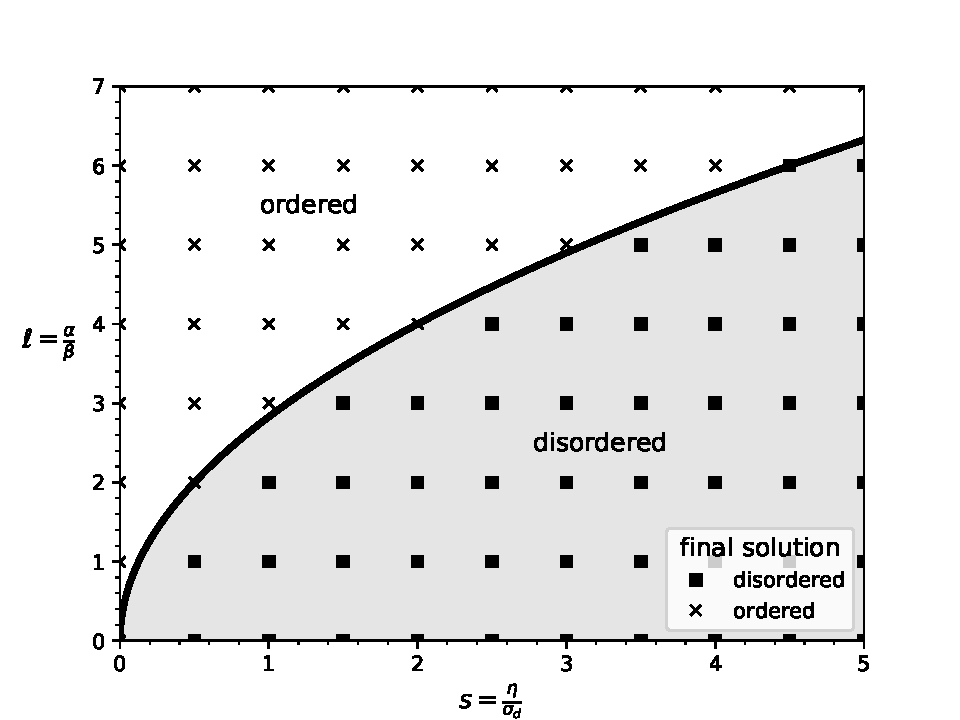
\includegraphics[width=0.7\linewidth, trim={0 0 0 1cm},clip=true]{figures/phase_diag_M2_sims}
	\caption{Phase diagram of a two-state adaptive network model as described by \cref{eq:M2system_closure_written_out}. The diagram displays the stable stationary state solution as a function of the dimensionless noise ratio $s=\frac{\eta}{\sigma_d}$ and the dimensionless link creation ratio $l=\frac{\alpha}{\beta}$. For $l<2\sqrt{2s}$, the disordered solution is stable, whilst for $l>2\sqrt{2s}$ the system will converge to the ordered solution. At the curve $l=2\sqrt{2s}$ there is a supercritical pitchfork bifurcation. Final distributions in numerical solutions for various $s$ and $l$ are indicated by the squares and crosses for the disordered and the ordered solution respectively. }
	\label{fig:phase_diag_M2}
\end{figure}


\chapter{Transformation to a continuous state set}
So far we have considered adaptive network models with a discrete state set $\Omega$, governed by a set of four dynamical rules. Recently there have been quite some publications on comparable discrete state (adaptive) network models, ranging from very fundamental mathematical backgrounds to applications of discrete state adaptive networks, for example \cite{Bauch2002,Chen2016,Demirel2014,Gross2006,Huepe2011,Keeling1999,Kimura2008,Newman2003,Sayama2013,Zschaler2012}. 
These models have however some drawbacks. For instance, if the network is used a model for self-organisation in a two-dimensional swarming system consisting of self-propelled particles, one could use $\Omega=\{\text{up}, \text{down}, \text{left}, \text{right}\}$. This means that diagonal motion would not be a separate state. A global diagonal movement would certainly be possible, but looking at a small time scale this movement would consist of small steps in two directions that are contained in $\Omega$. The problem with this is that the dynamics happen on the same small time scale as this flipping in states, such that a particle with a global diagonal movement to the north-west would interact half of the time similar with a particle moving north as a particle moving west would.

In this chapter, we make a transformation of discrete state networks to work on a continuous state set. The goal of making this transformation is to see if these networks might be a better model of reality in cases such as the aforementioned example. So far, limited research has been done into these type of networks. We derive the system of equations describing this class of models in a general form. 

This will be the most technical chapter of this thesis. The reader can skip ahead to \cref{chapter:swarming_systems} for the results. There, we will apply the derived model to self-organisation in two-dimensional swarming systems, where we have $\Omega = (-\pi,\pi]$ representing directions of 2D movement of self-propelled particles.

 
\section{State and link dynamics}
The continuous state adaptive network model will be derived in a general form. However to stay specific, some pre-determined properties will be applied to the model. The discrete state model is used as a starting point and from here we will make adaptations to make the model work on a continuous state set. We will write lower case letters for states contained in a continuous state set instead of upper case letters that are used for discrete states.  Starting with the types of dynamics, the dynamical rules used in the discrete state systems are not suitable anymore, hence they should be altered.  Especially the second type of state dynamics, where a triplet of nodes $y-x-y$ switches to state $y-y-y$ with rate $\sigma_d$ is not properly defined if we switch to continuous states; the probability for a node having two neighbours in the exact same state will be zero. Hence, the four types of interactions will be redefined for the continuous model:

\begin{description}
    \item [Type 1] Nodes change to another uniformly chosen state with rate $\eta$.
    \item [Type 2] Nodes adopt to the average state of two neighbours with rate $\sigma_c$. 
    \item [Type 3] Links are created between arbitrary not-linked nodes with rate $\alpha$.
    \item [Type 4] Links are removed between two arbitrary linked nodes with rate $\beta$.
\end{description}


\begin{figure}[t]
	\centering
	\begin{tikzpicture}[rotate=0]
	
	\draw[] (-5,0) node[circle, minimum size =0.5cm, draw] (state11) {};
	\draw[] (-3,0) node[circle, fill=black, minimum size =0.5cm, draw] (state12) {};
	
	\draw[->, shorten <=3pt, shorten >=3pt] (state11)--(state12) node[above, xshift=-1cm] {$\eta$};
	\draw[very thick] (state11)--(-5.4,0.8);
	\draw[very thick] (state11)--(-5.4,-0.8);
	\draw[very thick] (state12)--(-3.4,0.8);
	\draw[very thick] (state12)--(-3.4,-0.8);
	
	%%%%%%%%%%%%%%%%
	
	
	\draw[] (0,0) node[circle, pattern=soft crosshatch, minimum size =0.5cm, draw] (state21) {};
	\draw[] (-0.6,-1) node[circle, minimum size =0.5cm, draw] () {};
	\draw[] (1.4,-1) node[circle,minimum size =0.5cm, draw] () {};
	\draw[] (2,0) node[circle, fill=gray, minimum size =0.5cm, draw] (state22) {};
	\draw[] (-0.6,1) node[circle, fill=black, minimum size =0.5cm, draw] () {};
	\draw[] (1.4,1) node[circle, fill=black,minimum size =0.5cm, draw] () {};
	
	\draw[->, shorten <=3pt, shorten >=3pt] (state21)--(state22) node[above, xshift=-1cm] {$\sigma_c$};
	\draw[very thick] (state21)--(-0.45,-0.8);
	\draw[very thick] (state21)--(-0.6,1);
	\draw[very thick] (state22)--(1.55,-0.8);
	\draw[very thick] (state22)--(1.4,1);
	
	%%%%%%%%%%%%%%%%%%
	
	\draw[] (7,0.583) node[circle, fill=black, minimum size =0.5cm, draw] (link11) {};
	\draw[] (5,0.583) node[circle, fill=black, minimum size =0.5cm, draw] (link12) {};
	\draw[] (7,-0.583) node[circle, minimum size =0.5cm, draw] (link13) {};
	\draw[] (5,-0.583) node[circle, minimum size =0.5cm, draw] (link14) {};
	
	\draw[very thick] (link11)--(link13);
	
	\draw[->, shorten <=3pt, shorten >=3pt, transform canvas={yshift=-0.683cm}] (link11)--(link12) node[below, xshift=1cm] {$\beta$};
	\draw[->, shorten <=3pt, shorten >=3pt, transform canvas={yshift=-0.483cm}] (link12)--(link11) node[above, xshift=-1cm] {$\alpha$};
	
	\end{tikzpicture}
	\caption{Illustration of the model, four types of dynamics are applied to the continuous state adaptive network models.  The internal state of each node (circle) is represented by its colour. The grey colour corresponds to the average of the states black and white. The chequered pattern indicates a random state in the state set $\Omega$. These dynamics take place irrespective of any additional links that may be present, but are not drawn.}
	\label{fig:dynamics_continuous}
\end{figure}
The dynamics take place irrespective of any additional links that may be connected to a node. Furthermore, we cannot use the same definition of densities for nodes and small subgraphs as before. These discrete network moments would not be properly defined if a system of continuous states is considered. Therefore state and link density functions will be introduced. These functions describe the distribution of the possible states in the network (comparable to probability density functions in probability theory). In order to introduce these formally, let us first consider the cumulative distribution functions $F(x;t)$ and $L_n(x_1,x_2,...,x_n;t)$ and assume that the state set $\Omega$ is a single non-empty, bounded real interval. That is $\Omega = [a,b]$, or $\Omega = (a,b)$, where $a,b \in \mathbb{R}$ and the endpoints are either included in or excluded from the interval. 
\begin{definition}
	The cumulative distribution function (CDF) $F(x;t)$ denotes the density of nodes that have a state in $[a, x] \subseteq \Omega$ at time $t$. 
\end{definition}
\begin{definition}
	Let $n\in\mathbb{N}\setminus\{1\}$. For $n$-body subgraphs (e.g. links, triplets etcetera) the $(n-1)$'th order moment cumulative distribution function $L_n(x_1,x_2,...,x_n;t)$ is the density of motifs in which the first node occupies a state in $[a, x_1]$, which is connected to a second node occupying a state in $[a, x_2]$, etcetera, at time $t$.
\end{definition}

CDFs can be defined analogously for open intervals. The node density, but also the higher order densities are all normalised against the total number of nodes $N$. The density of nodes in a certain state is a zeroth-order moment, the density of e.g. $x-y$-links a first-order moment and the density of subgraphs consisting of $n$ nodes an $(n-1)$'th-order moment. Subsequently, the state and link density distribution functions can be defined as follows.  
\begin{definition}
	The state distribution function $f(x;t) : \Omega \times \mathbb{R}_{\ge0} \to  \mathbb{R}_{\ge0}$ is the unique function that satisfies $F(x;t) = \int\limits_a^x d\bar{x}\ f(\bar{x};t)$.
\end{definition}
\begin{definition}
	The $(n-1)$'th order moment distribution function $l_n(x_1,x_2,...,x_n;t): \Omega^n \times \mathbb{R}_{\ge0} \to  \mathbb{R}_{\ge0}$ is the unique function that satisfies $L_n(x_1,x_2,...,x_n;t) = \int\limits_a^{x_{1}} d\bar{x_1} \int\limits_a^{x_{2}} d\bar{x_2}\ ... \int\limits_a^{x_n} d\bar{x_n}\  l(\bar{x_1}, \bar{x_2},...,\bar{x_n};t)$.
\end{definition}
In these definitions, $\bar{x}$ and $\bar{x_i}, i \in \{1,2,...,n\}$, are used as integration variables. Note that the link distribution functions obey a certain symmetry. By definition $l_2(x,y;t) = l_2(y,x;t)$, which makes sense since if an $x$-node is connected to a $y$-node, one can describe the links both as an $x-y$- or as an $y-x$-link. Moreover, we have $l_3(x,y,z;t) = l_3(z,y,x;t)$, both representing the density of $x-y-z$-triplets.  Furthermore, we remark that the distribution functions do not have to be continuous in state space. However, in case a distribution function is continuous in state space, we have $f(x;t) = \frac{\partial}{\partial x} F(x;t)$ and $l_n(x_1,x_2,...,x_n;t) = \frac{\partial}{\partial x_1} \frac{\partial}{\partial x_2} ... \frac{\partial}{\partial x_n} L(x_1, x_2,...,x_n)$. Intuitively $f(x;t)dx$ is the density of nodes occupying a state within the interval $[x,x+dx]$, while $ l_n(x_1, x_2,...,x_n;t)dx_1dx_2...dx_n$ is the density of $n$ body subgraphs with the first node in state $[x_1,x_1+dx_1]$ is connected to a second node in state $[x_2,x_2+dx_2]$, etcetera. 

Besides, it will be useful to derive a density distribution function for subgraphs in configuration $^wx^y_z$, with the middle node in state $x$ connected to nodes in states $w,y$ and $z$. 
\begin{definition}
	The third order moment distribution $l(^wx^y_z;t): \Omega^4 \times \mathbb{R}_{\ge0}  \to \mathbb{R}_{\ge0}$ describes the density of subgraphs in configuration $^wx^y_z$ at time $t$.
\end{definition}
We will derive the equations describing the effect of the four types of dynamics on the state and link distributions in the most general form possible, such that they can be applied to model a great variety of phenomena. To keep things clear the equations will be introduced for each type of dynamics separately. The effect of the dynamics of type 1 on the state density function $f(x;t)$ are captured by the following partial differential equation (PDE). The superscript $(1)$ indicates that only the dynamics of the first type are captured by this equation.
\begin{equation}
\begin{aligned}
    \frac{\partial f^{(1)}(x;t)}{\partial t} 
    &= -  \eta \ f(x;t) + \frac{\eta}{\Vert \Omega \Vert}  \int\limits_{\Omega \setminus \{x\}} d\bar{x} \ f(\bar{x};t) \\
    &= - \eta\ f(x;t) + \frac{\eta}{\Vert \Omega \Vert} \int\limits_{\Omega} d\bar{x}\ f(\bar{x};t)  \\
    &= \eta \left( \frac{1}{\Vert \Omega \Vert} - f(x;t) \right),
    %&= \eta \left( \frac{1}{2\pi} - f(x;t) \right),
    \label{eq:continuous_pde_state_firsttype}
\end{aligned}
\end{equation}
where we used $\bar{x}$ as integration variable which is integrated over the complete set of states, except for state $x$. The first term corresponds to nodes leaving state $x$ for another uniformly chosen state and the second term to nodes changing spontaneously to state $x$. Note, since the density function integral in a point equals zero the integral over $\Omega \setminus \{x\}$ equals the integral over the complete set $\Omega$. The expression should be divided by the total size of the set $\Vert \Omega \Vert$, as the node should change to the specific state $x$. In the last step, we made use of the fact that the integral of a state density function over the complete set of states equals 1. 

It can easily be observed that the solution to \cref{eq:continuous_pde_state_firsttype} converges to the uniform distribution density function, that is $ \lim\limits_{t \to \infty} f(x;t) = \frac{1}{\Vert \Omega \Vert}$. In particular, if $f(x;t) > \frac{1}{\Vert \Omega \Vert}$ we have $\frac{\partial f(x;t)}{\partial t} < 0$ and vice versa. 

The change in link density $l_2(x,y;t)$ due to interactions of type 1 is described by the following PDE. From now on we will write $\int\limits_{\Omega \setminus \{x\}}$ directly as $\int\limits_{ \Omega}$. We have
\begin{equation}
\begin{aligned}
    \frac{\partial l_2^{(1)}(x,y;t)}{\partial t} 
    &= - 2\eta\ l_2(x,y;t) + \frac{\eta}{\Vert \Omega \Vert} \int\limits_{\Omega}dz\ l_2(z,y;t)   + \frac{\eta}{\Vert \Omega \Vert} \int\limits_{\Omega}dz\ l_2(x,z;t)    \\
 %   &=  - 2\eta\ l_2(x,y;t) + \frac{\eta}{2\pi} \int\limits_{\Omega}dz\ l_2(z,y;t)   + \frac{\eta}{2\pi} \int\limits_{\Omega}dz\ l_2(x,z;t)\\ 
    &= - 2\eta \ l_2(x,y;t) + \frac{\eta}{\Vert \Omega \Vert} \int\limits_{\Omega}dz\ \left( l_2(z,y;t)   +  l_2(x,z;t) \right)  
    ,
    \label{eq:continuous_pde_link_firsttype}
\end{aligned}
\end{equation}
in which the second and third term correspond to the creation of $x-y$-links. That is $z-x$- and $z-y$-links with an arbitrary $z \in \Omega$ changing to $y$ or $x$ respectively. The first term describes the destruction of $x-y$-links due to one of the nodes changing to another state, hence the factor~2. The last simplification step is justified by the linearity property of the Riemann integral.

Equations (\ref{eq:continuous_pde_state_firsttype}) and (\ref{eq:continuous_pde_link_firsttype}) describe a continuous system which obeys interactions of the first type only. The next step will be to obtain similar equations for the second type of dynamics. For the state density $f(x;t)$, these interactions can be described as follows,
\begin{equation}
\begin{aligned}
\frac{\partial f^{(2)}(x;t)}{\partial t} 
&= \sigma_c \int d \xi  \int\limits_{\Omega}dz\ l_3(x-\xi ,z,x+\xi ;t)   - \sigma_c \int d\xi \ \int\limits_{\Omega} dz\ l_3(z-\xi,x,z+\xi;t) \\
&= \sigma_c \int\limits_{\Omega}dz\ \int d \xi\ \left( l_3(x-\xi ,z,x+\xi ;t)   - l_3(z-\xi,x,z+\xi;t) \right)
.
\label{eq:continuous_pde_state_secondtype}
\end{aligned}
\end{equation}
The first term represents nodes in an arbitrary state $z$, in between two nodes in states $x-\xi $ and $x+\xi $ such that their average state is $x$. This way an extra $x$ node is created due to three-body interactions at rate $\sigma_c$. The second term corresponds to removal of $x$ nodes due to these interactions. We take an $x$ node in between two arbitrary nodes in states $z+\xi$ and $z-\xi$. Their average state is $z$, which is in general not equal to $x$, which justifies the integration over the complete state set $\Omega$. The simplification step is again justified by linearity of the integral and moreover by Fubini's double integral theorem \cite{Fubini1907}.
However, we should be careful, since the integral boundaries may demand function evaluations outside of the domain on which the density functions are defined. In that case, there are two different ways to compute the integrals, depending on the application. The state set can be a normal interval $\Omega =[a,b]$. Then we simply define all density distributions to be zero outside the state set $\Omega$, such that the integrals can be evaluated. Another possibility is that the state set is periodic, for example $\Omega =[-\pi,\pi)$, with $x+2\pi=x$ for all $x\in\Omega$. We want the integrals to take this periodicity into account. Hence, we would make even extensions of the density distribution functions at the boundaries of the state set. In the next part of this thesis, we will elaborate on making the system specific for application on such a periodic state set.

The next partial differential equation captures the change in the link density function $l_2(x,y;t)$ due to the three-body interactions 
\begin{equation}
\begin{aligned}
\frac{\partial l^{(3)}_2(x,y;t)}{\partial t} 
=& \phantom{+..}
   \sigma_c \int\limits_{\Omega} dz \int d\xi\ l_4(^y z^{x-\xi }_{x+\xi };t) \\
&+ \sigma_c \int\limits_{\Omega} dz \int d\xi\ l_4(^x z^{y-\xi }_{y+\xi };t)  \\
&- \sigma_c \int\limits_{\Omega} dz \int d\xi\ l_4(^y x^{z-\xi}_{z+\xi};t) \\
&- \sigma_c \int\limits_{\Omega} dz \int d\xi\ l_4(^x y^{z-\xi}_{z+\xi};t) \\
&+ \sigma_c \int\limits_{\Omega} dz\ l_3(y,z,-y+2x;t) \\
&+ \sigma_c \int\limits_{\Omega} dz\ l_3(x,z,-x+2y;t) \\
&- \sigma_c \int\limits_{\Omega} dz\ l_3(y,x,z;t) \\ 
&- \sigma_c \int\limits_{\Omega} dz\ l_3(x,y,z;t) 
.
\label{eq:continuous_pde_link_secondtype}
\end{aligned}
\end{equation}
The first term represents four-body subgraphs of configuration $^y z^{x-\xi }_{x+\xi }$ in which the middle node $z$ changes to the average state of $x-\xi $ and $x+\xi $, which is $x$. Here, one $x-y$-link is created with the neighbouring $y$ node. We integrate over all $z \in\Omega$ to include all nodes which might change to state $x$. Again, we integrate over all $\xi $ for which our averaging operation is defined properly. The second term is quite similar. Here, the positions of nodes in state $x$ and $y$ are inverted. 
The third term corresponds to four-body subgraphs of configuration $^y x^{z-\xi }_{z+\xi }$. Now, the middle node takes with rate $\sigma_c$ the average of the two neighbouring nodes $z-\xi$ and $z+\xi$, which is $z$ and does not equal $x$ in general. This causes the $y-x$-link to be changed in a $y-z$-link, explaining the minus sign. The fourth term is again similar to the third one.
Three-body subgraphs with the potential to form an $x-y$-link are taken into account in the fifth and sixth term. In triplets with configuration $y-z-(-y+2x)$ and $x-z-(-x+2y)$ the middle node takes the average value of the outer two, which is $x$ or $y$ respectively, with rate $\sigma_c$. With this, an $x-y$-link is created with the already existing $y$ or $x$ node.
Three-body subgraphs $x-y-z$ and $y-x-z$ are taken into account in the last two terms. The middle node takes the average state of the outer two, which is again in general not $x$ or $y$. We integrate over all $z\in\Omega$ to include all subgraphs of this form. Note, $l_3(x,y,z;t)=l_3(z,y,x;t) \ne l_3(y,x,z;t)$. Note too that this equation is still an approximation. There could always be more terms added. However, these terms would correspond to subgraphs with a very specific configuration. We assume that the densities of these subgraphs are small compared to the other terms, such that they can be omitted.

The next step will be adding the link dynamics. Equations (\ref{eq:continuous_pde_state_thirdtype}) and (\ref{eq:continuous_pde_link_thirdtype}) describe the link creation interactions. Since the node states do not change when adding links, we have
\begin{equation}
\begin{aligned}
    \frac{\partial f^{(3)}(x;t)}{\partial t} 
    &= 0
    .
    \label{eq:continuous_pde_state_thirdtype}
\end{aligned}
\end{equation}
Moreover, the fact that links are created between two arbitrary nodes with rate $\alpha$ is described as 
\begin{equation}
\begin{aligned}
    \frac{\partial l^{(3)}_2(x,y;t)}{\partial t} 
    &= \alpha \ f(x;t)\ f(y;t)
    .
    \label{eq:continuous_pde_link_thirdtype}
\end{aligned}
\end{equation}

The deletion of links is described by similar PDEs. Again, the node states stay unchanged, yielding
\begin{equation}
\begin{aligned}
    \frac{\partial f^{(4)}(x;t)}{\partial t} 
    &= 0,
    \label{eq:continuous_pde_state_fourthtype}
\end{aligned}
\end{equation}
whilst the removal of arbitrary links with rate $\beta $ is captured by 
\begin{equation}
\begin{aligned}
    \frac{\partial l^{(4)}_2(x,y;t)}{\partial t} 
    &= -\beta\ l_2(x,y;t)
    .
    \label{eq:continuous_pde_link_fourthtype}
\end{aligned}
\end{equation}



%%%%%%%%%%%%%%%%%%%%%%%%%%%%%%%%%%%%%%%%%%%%%%%%%%%%%%%%%%%%%%%%%%%%%%%%%%%%%%%%%%%%%%%%%




\section{Completing the continuous model}

Equations (\ref{eq:continuous_pde_state_firsttype}) - (\ref{eq:continuous_pde_link_fourthtype}) describe the influence of the four types of interactions on the time derivatives of the state and link density functions. To obtain the complete model, these PDEs can simply be added. This yields the following equation for the state density function
\begin{equation}
\begin{aligned}
	\frac{\partial f(x;t)}{\partial t}  
	=& \frac{\partial f^{(1)}(x;t)}{\partial t}  + \frac{\partial f^{(2)}(x;t)}{\partial t}  + \frac{\partial f^{(3)}(x;t)}{\partial t}  + \frac{\partial f^{(4)}(x;t)}{\partial t} \\
	=&\ \eta \left( \frac{1}{\Vert \Omega \Vert} - f(x;t) \right) \\
	&+  \sigma_c \int\limits_{\Omega}dz\  \int d \xi \ \left( l_3(x-\xi ,z,x+\xi ;t)  - l_3(z-\xi,x,z+\xi;t) \right)
	.
	\label{eq:continuous_pde_state_complete_w_ho_terms}
\end{aligned}
\end{equation}

\raggedbottom

The PDE describing the link density function can be obtained in a similar fashion
\begin{equation}
\begin{aligned}
	\frac{\partial l_2(x,y;t)}{\partial t} 
	=& \frac{\partial l^{(1)}_2(x,y;t)}{\partial t} + \frac{\partial l^{(2)}_2(x,y;t)}{\partial t} + \frac{\partial l^{(3)}_2(x,y;t)}{\partial t} + \frac{\partial l^{(4)}_2(x,y;t)}{\partial t}\\
	=&\
	\frac{\eta}{\Vert \Omega \Vert} \int\limits_{\Omega}dz\ \left( l_2(z,y;t)   +  l_2(x,z;t) \right) \\
	&+ \sigma_c \int\limits_{\Omega} dz \int d \xi \ \left( l_4(^y z^{x-\xi}_{x+\xi};t) +  l_4(^x z^{y-\xi}_{y+\xi};t) \right)  \\
	&- \sigma_c \int\limits_{\Omega} dz \int d \xi \ \left( l_4(^y x^{z-\xi}_{z+\xi};t) +  l_4(^x y^{z-\xi}_{z+\xi};t) \right) \\
	&+ \sigma_c \int\limits_{\Omega} dz\ \left( l_3(y,z,-y+2x;t) + l_3(x,z,-x+2y;t)  \right) \\
	&- \sigma_c \int\limits_{\Omega} dz\ \left( l_3(y,x,z;t)     + l_3(x,y,z;t)      \right) \\
	&+ \alpha \ f(x;t)\ f(y;t) \\
	&- (2\eta + \beta) \ l_2(x,y;t)
	,
	\label{eq:continuous_pde_link_complete_w_ho_terms}
\end{aligned}
\end{equation}
where again the linearity of the Riemann integral was used to simplify the expression. Equations (\ref{eq:continuous_pde_state_complete_w_ho_terms}) and (\ref{eq:continuous_pde_link_complete_w_ho_terms}) together describe the adaptive network model with a continuous state set in the most general form. There are two main differences with the discrete adaptive networks. Firstly, the types of dynamics had to be slightly altered. Secondly, the network evolution is described by partial (integro-)differential equations, instead of ordinary differential equations. Although these are in general harder to solve, there are only two coupled equations. For the discrete state set we needed $M(2+\frac{1}{2}(M-1))$ coupled equations for $M$ states.

Note however, that not all terms are known. Just as in the discrete adaptive networks, moment equations of a given order are dependent on higher order terms. One might think this means we need extra PDEs for these higher order moments, but then we would go on until we get equations for subgraphs of size in the order of the network size, resulting in a system of a large amount connected PDEs which would be very hard to solve. Moreover, numerical estimates would not allow for developing an analytical solution. This can be prevented in multiple ways. In the next sections, two possibilities are described: the mean field approximation and the moment closure approximation, both were also applied for the discrete state adaptive networks in the first part of this work.  

%%%%%%%%%%%%%%%%%%%%%%%%%%%%%%%%%%%%%%%%%%%%%%%%%%%%%%%%%%%%%%%%%%%%%%%%%%%%%%%%%%%%%



\section{Mean Field model}
A first approach into solving a continuous state adaptive network model would be considering a mean field approximation. This is equivalent to neglecting the link dynamics and assuming that the density of links connecting nodes in a given state is proportional to the product of the densities of these states, similar what was done to the discrete state adaptive networks. This simplifies \cref{eq:continuous_pde_state_complete_w_ho_terms} to the following mean field approximation 


\begin{equation}
\begin{aligned}
\frac{\partial}{\partial t}\ f(x;t) &= 
\eta \left( \frac{1}{\Vert \Omega \Vert} - f(x;t) \right) \\ 
&+ \sigma_c\langle k \rangle^2 \int\limits_{\Omega} dz \int\limits d\xi\
f(x-\xi;t)\ f(z,t)\ f(x+\xi;t) \\
&- \sigma_c \langle k \rangle^2 \int\limits_{\Omega} dz  \int\limits_{\Omega} dw\ f(w;t)\ f(x;t)\ f(z;t),
\end{aligned}
\end{equation}
where $\bar{x}$ is used as an integration variable and in which $\langle k \rangle$ is the aforementioned proportionality constant, representing the mean network degree. Since we are dealing with a density function, $\int\limits_{\Omega} dx\ f(x;t) =1$, such that we can simplify to
\begin{equation}
\begin{aligned}
\frac{\partial}{\partial t}\ f(x;t) &= 
\eta \left( \frac{1}{\Vert \Omega \Vert} - f(x;t) \right) \\
&	+ \sigma_c\langle k \rangle^2  \int\limits d\xi\
f(x-\xi;t)\ f(x+\xi;t) \\
&	- \sigma_c \langle k \rangle^2\ f(x;t) \int\limits_{\Omega} dz \int\limits d\xi\ f(z-\xi;t)\ f(z+\xi;t).
\end{aligned}
\label{eq:cont_state_mean_field}
\end{equation}
Since link dynamics are neglected in the mean field approximation there is no need to approximate \cref{eq:continuous_pde_link_complete_w_ho_terms}. Therefore, the mean field system is described with only one partial integro-differential equation, which has the advantage that it allows for easier analysis compared to a system of PDEs. In \cref{chapter:swarming_systems} we apply the mean field model to two-dimensional swarming motion of self-propelled particles.

\section{Moment closure approximation}
In order to obtain the system of two coupled, closed PDEs we seek expressions for the unknown terms $l_3(x,y,z;t)$ and $l_4(^x y^z_w;t)$ in terms of the known lower order moments $l_2(x,y;t)$ and $f(x;t)$. Analogous to the discrete state adaptive network models, the closure used will be the pair level closure, 
\begin{align}
l_3(x,y,z;t) & = \frac{l_2(x,y;t)\ l_2(y,z;t)}{f(y;t)},\\
l_4(^x y^z_w;t) &= \frac{l_2(x,y;t)\ l_2(y,z;t)\ l_2(y,w;t)}{f(y;t)^2},	
\end{align}
which is elaborated on in the first part of this thesis. Additional derivation and explanation can be found in \cite{Chen2016, Demirel2014, Newman2003}. We will assume that this closure relation is still valid in the continuous state case.
Applying the approximation would result in a closed system of two coupled PDEs, one for the state density function $f(x;t)$ and one for the first order link density function $l_2(x,y;t)$. Hence, it will be convenient to write  $l_2(x,y;t) =  l(x,y;t)$ from now on. With this approximation, the adaptive network models with a continuous state set are captured by the following two coupled non-linear partial integro-differential equations

\begin{subequations}\label{eq:cont_complete}
\small
\begin{adjustwidth}{-.5in}{-.5in} 
	\begin{alignat}{2}
	\frac{\partial f(x;t)}{\partial t} = &
	\ \eta \left( \frac{1}{\Vert \Omega \Vert} - f(x;t) \right) \\
	& + \sigma_c\int\limits_{\Omega} dz \int\limits  d \xi  \
	\Bigg[ 
	\frac{l(x-\xi ,z;t)\ l(z,x+\xi ;t)}{f(z;t)} - \frac{l(z-\xi ,x;t)\ l(x,z+\xi ;t)}{f(x;t)} 
	\Bigg]  \nonumber \\[15pt] 
	\frac{\partial l(x,y;t)}{\partial t} = &
	\int\limits_{\Omega} dz \
	\Bigg{\{ }
	\frac{\eta}{\Vert \Omega \Vert} \left( l(x,z;t) + l(z,y;t) \right)   \\
	& \phantom{\int\limits_{\Omega} dz\ \sum}
	+\sigma_c \frac{l(y,z;t)\ l(z,-y+2x;t)}{f(z;t)}
	+\sigma_c \frac{l(x,z;t)\ l(z,-x+2y;t)}{f(z;t)} \nonumber \\
	& \phantom{\int\limits_{\Omega} dz\ \sum}
	-\sigma_c \frac{l(y,x;t)\ l(x,z;t)}{f(x;t)} 	 
	-\sigma_c \frac{l(x,y;t)\ l(y,z;t)}{f(y;t)} \nonumber \\
	& \phantom{\int\limits_{\Omega} dz\ \sum}
	+ \sigma_c\int\limits d \xi \    
	\Bigg[  
	\frac{l(y,z;t)\ l(z, x-\xi;t)\ l(z, x+\xi;t)}{f(z;t)^2}  + 
	\frac{l(x,z;t)\ l(z, y-\xi;t)\ l(z,y+\xi ;t)}{f(z;t)^2} \nonumber  \\ 
	& \phantom{\int\limits_{\Omega} dz\ \sum \sigma_c\int\limits \ d \xi \sum }
	- \frac{l(y,x;t)\ l(x, z-\xi;t)\ l(x,z+\xi ;t)}{f(x;t)^2} - 
	\frac{l(x,y;t)\ l(y, z-\xi ;t)\ l(y, z+\xi ;t)}{f(y;t)^2} 
	\Bigg]	 \
	\Bigg{ \} } \nonumber \\
	&+ \alpha\ f(x;t)\ f(y;t) - 
	(2\eta+\beta)\ l(x,y;t).\nonumber
	\end{alignat}
\end{adjustwidth}
\end{subequations}
\normalsize


\chapter{Modelling swarming systems}
\label{chapter:swarming_systems}
With swarming systems, we indicate the class of all processes of collective motion. From the most specific processes, which are for example the dynamics in a flock of birds, a school of fish or the behaviour of a crowd of people, to the most general processes, such as collective motion in systems of self-propelled particles, which obey certain prescribed interaction rules. The process of self-organisation in such systems is still poorly understood. So far, research into swarming systems was mainly done in either of two ways. The swarm was represented as a continuous medium \cite{Toner1998}, or (comprehensive) agent-based models were developed that obey certain dynamical rules \cite{Huepe2011, VanDrongelen2015, Vicsek1995, Vicsek2012}. Since a few years, research into the application of adaptive networks on swarming systems has gotten more attention \cite{Huepe2011, Chen2016, Zschaler2012}. In the next section, we will apply the developed continuous state adaptive network model to a swarming system.

The most famous minimal agent-based model of collective motion is the Vicsek model \cite{Vicsek1995}. It describes a system of self-propelled individuals moving at a constant speed $v$. These individuals try to align with all their neighbours within a certain radius $r$, such that the system can be (discretely) evolved as 
\begin{subequations}
\begin{alignat}{2}
	\bm{x_i}(t+\Delta t) &= \bm{x}_i(t) + \bm{v}_i \Delta t\\
	\theta_i(t+\Delta t) &= \langle \theta_j \rangle_{|r_i - r_j | <r} + \eta_i
\end{alignat}
\end{subequations}
in which $\bm{x_i}(t)$ represents the position of the $i$'th individual at time $t$. The direction of its velocity is given by $\theta_i(t)$. $\eta_i$ is a noise parameter, which can for example be drawn from a uniform probability distribution on the interval $(-\pi,\pi]$.

Although many great advances have been made with (variations on) the Vicsek model \cite{Vicsek2012}, there is a restriction on the size of the system. The position and direction of each individual should be updated each time step, which may lead to computationally heavy simulations. For adaptive networks, there is no such limit. The accuracy even improves for increasing system size, such that these models allow for obtaining more general results. Therefore, modelling swarming systems in an adaptive network might give new insights into the self-organisation in large swarming systems. 


\section{Applying the developed adaptive network models to swarming systems}
\label{section:applying_network_to_swarming}
So far, the adaptive network models have been derived in the most general form possible. In the last part of this thesis, we will apply them to swarming systems of two-dimensional motion. All individuals are represented by a node and individuals that are aware of each other's behaviour are connected by a link. This allows for a very similar condition to the alignment in the Vicsek model, where individuals tend to align with their neighbours within a certain radius. We will refer to individuals connected by a link as neighbours. Moreover, we assume that all individuals can be modelled as self-propelled particles with a constant speed $v$, such that only their direction of movement is of importance. In this work, we will restrict the individuals to move in two dimensions only. Hence, it would be a sensible choice to define $\Omega = (-\pi,\pi]$. Furthermore, we can make the four types of interactions more specific:

\begin{description}
	\item [Type 1] Individuals pick another direction with rate $\eta$. This direction is uniformly chosen from $\Omega = (-\pi,\pi]$
	\item [Type 2] Individuals adopt to the average direction of two neighbours with rate $\sigma_c$.
	\item [Type 3] Arbitrarily chosen not-neighbouring individuals become neighbours with rate $\alpha$.
	\item [Type 4] Arbitrarily chosen neighbours become not-neighbouring individuals with rate $\beta$.
\end{description}

All dynamics take place irrespective of any additional neighbours an individual may have. A swarming system can be well described with these four types of interactions. The first two types are comparable to the Vicsek model; type 1 is similar to the noise $\eta_i$ of the $i$'th particle, whereas type 2 corresponds to the tendency of individuals to align with their neighbours within a certain radius. This radius is in the network modelled with the links since we do not keep track of the physical position of individuals in space. Interactions of the third type are needed since not-neighbouring individuals which move in different directions might become aware of each other's position at a certain moment. It is sufficient to model this by a global rate because we do not look at individual nodes separately (which would also not be possible since we do not know the individuals' physical position). The main advantage here is that this allows for faster computations. The fourth type of dynamics is the opposite of the third type; individuals which are neighbouring, but head in different directions are at a certain moment too far apart to be still aware of each other. Therefore their link must be broken. Again, it is sufficient to model this with a global rate. 

In this case, the meaning of the state distribution function $f(x;t)$ can be explained as follows: the network density of individuals with direction $x$ in the interval $[\theta_1,\theta_2]$ at time $t$ is given by 
\[
\int\limits_{\theta_1}^{\theta_2} d\bar{x}\ f(\bar{x};t).
\]
For the link distribution function $l(x,y;t)$ we have something similar: the density of pairs of neighbouring individuals, where one of the neighbours' direction $x$ is within the interval $[\theta_1,\theta_2]$, while the other heads in a direction $y$ in the interval $[\phi_1,\phi_2]$, at time $t$, is given by 
\[
\int\limits_{\theta_1}^{\theta_2} d\bar{x}\ \int\limits_{\phi_1}^{\phi_2} d\bar{y}\ l(\bar{x},\bar{y};t).
\]

So far, we have not mentioned how the averaging operation in the model is defined, because this definition can differ for various applications. This operation corresponds to the integrals over $\xi$ in \cref{eq:cont_complete}. In the case of two-dimensional motion, the average should be taken in a special way, because the interval is periodic. This is easiest illustrated in an example. Suppose one individual has a direction of $\theta_1=\frac{3\pi}{4}$, while another individual moves in the $\theta_2 = -\frac{3\pi}{4}$ direction. The numerical average would be zero, while the `angular' average is $\theta=\pi$. In this case, we clearly should use the latter. This can be implemented in the equations by integrating over $\xi$ from $0$ to $\frac{\pi}{2}$, instead of integrating over the complete state set $\Omega$.  \Cref{fig:cont_states_averaging_k} illustrates this process of finding the right states which average direction $x$. Every pair of individuals heading in directions $x-\xi$ and $x+\xi$ respectively have the possibility to let a common neighbour change its direction to $x$ as long as $\xi \in \left[0,\frac{\pi}{2}\right)$.


\begin{figure}[t]
	\centering
	\begin{tikzpicture}[rotate=30]
	\draw[thick] (0,0) coordinate(O) circle (3);
	\draw[dashed] (-3.2,0) node[left] {$x-\frac{\pi}{2}$} -- (3.2,0) node[right] {$x+\frac{\pi}{2}$};
	\draw (0,-3) coordinate(under) node[below,xshift=0.1cm] {$x$} -- (0,0); 
	\draw[rotate=35] (-3,0) coordinate(left) node[left, yshift=-0.2cm] {$x-\xi $} -- (0,0);
	\draw[rotate=-35] (0,0) -- (3,0) coordinate(right) node[right] {$x+\xi $};
	\draw pic["$\xi $", <-, draw, thick,angle radius=10mm] {angle = left--O--under};% node[xshift=0cm, yshift=-1.3cm] {$\xi $};
	\draw pic["$\xi $", ->, draw, thick,angle radius=12mm] {angle = under--O--right};% node[xshift=1.25cm, yshift=-0.85cm] {$\xi $};
	\end{tikzpicture}
	\caption{The process of finding the right directions $x-\xi $ and $x+\xi $ which average to $x$. Clearly $\xi \in \left[0,\frac{\pi}{2}\right)$ or the average will be in the direction $x+\pi$.}
	\label{fig:cont_states_averaging_k}
\end{figure}

Now we have all variables, functions and dynamics rules properly defined to apply the previously derived network to swarming systems. In the next two sections, the resulting sets of equations for both the mean field approximation and the moment closure approximation models are stated, including results and corresponding analysis.

\section{Mean field approximation on swarming systems}
All rules making the continuous state adaptive network model a swarming system were described in the previous section. In this section, they will be applied to the mean field approximation. Subsequently, analysis and discussion of the results will follow. 

The partial differential \cref{eq:cont_state_mean_field} models the collective motion in the previously described swarm if we write it as 

\begin{equation}
\begin{aligned}
\frac{\partial}{\partial t}\ f(x;t) =\ & 
\eta \left( \frac{1}{2\pi} - f(x;t) \right) \\
&	+ \sigma_c\langle k \rangle^2  \int\limits_{0}^{\pi/2} d\xi\
f(x-\xi;t)\ f(x+\xi;t) \\
&	- \sigma_c \langle k \rangle^2\ f(x;t) \int\limits_{-\pi}^\pi dz \int\limits_{0}^{\pi/2} d\xi\ f(z-\xi;t)\ f(z+\xi;t).
\label{eq:cont_state_mean_field_swarming}
\end{aligned}
\end{equation}


\subsection{Discretisation}
It is unlikely that we can find the time-dependent solution to this equation analytically, consequently let us look for a numerical solution. The first step will be discretising the time and state set $\Omega$. This will yield a partial \textit{difference} equation which can be solved using a computer.
The continuous time $t = [0, T_{\text{max}}]$ at which the network evolution is considered will be partitioned into $M$ intervals of length $\Delta t$, such that the discrete time set is of the form 
\[ t_d= \{0, \Delta t, 2 \Delta t, ... , (\tau-1) \Delta t,  \tau\Delta t, ..., T_{\text{max}} - \Delta t, T_{\text{max}}  \}, \]
in which $M \Delta t = T_{\text{max}}$ and $\tau$ is the discrete time index. Next, we have to discretise the state set $\Omega$. This set is partitioned into $N$ intervals of length $\Delta \omega$, such that $\Omega = (-\pi,\pi]$ is transformed into 
\[\Omega_d = \{-\pi, -\pi+\Delta\omega,...,-\pi+ (p-1) \Delta\omega, -\pi+ p \Delta\omega, ... \pi-\Delta\omega, \pi \}, \]
in which $N \Delta \omega = 2\pi$ and $p$ is the discrete state index.\footnote{It might seem odd to discretise the state set as we have just made it continuous. Ironically this is the first step in solving the system numerically. It is however important to note that the discretisation is different from the discrete state model. This discretisation gives the same solutions as the continuous state model would if it were solved analytically if we take the limits of $\Delta t \to 0$ and $\Delta \omega \to 0$. Moreover, it incorporates the different dynamics which are used exclusively in the continuous state case. In other words, we are really solving a different system.}
Furthermore, we use the following shorthand notation in the discretisation of the density function $f(x;t)$, 
\[
f_{p}^{\tau } = f(-\pi+p\Delta \omega; \tau \Delta t).
\]
The discrete state-time-grid which is obtained is visualised in \cref{fig:grid_pde}.

\begin{figure}[htp]
	\centering
	\begin{tikzpicture}[dot/.style={draw,circle,minimum size=0.6mm,inner sep=0pt,outer sep=0pt,fill=black}]
	\path \foreach \x/\y [count=\k from 0] in { 0/0,  1/0, 2/0, 3/0, 4/0, 5/0, 6/0, 7/0, 0/1,  1/1, 2/1, 3/1, 4/1, 5/1, 6/1, 7/1, 0/2,  1/2, 2/2, 3/2, 4/2, 5/2, 6/2, 7/2, 0/3,  1/3, 2/3, 3/3, 4/3, 5/3, 6/3, 7/3,0/4,  1/4, 2/4, 3/4, 4/4, 5/4,6/4, 7/4,0/5,  1/5, 2/5, 3/5, 4/5, 5/5,6/5,7/5, 0/6,1/6,2/6,3/6,4/6,5/6,6/6, 7/6}
	{coordinate [dot] (p\k) at (\x,\y)}; 
	
	\draw[->] (6.7,-0.5)--(7,-0.5) node[below] at (3.5,-1) {$t$};
	\draw[] (0,-0.5)--(0.3,-0.5);
	\draw[] (0.7,-0.5)--(6.3, -0.5);
	\draw[dotted] (0.3,-0.5)--(0.7,-0.5);
	\draw[dotted] (6.3,-0.5)--(6.7,-0.5);
	
	\draw[->] (-0.5,5.7)--(-0.5,6) node[left] at (-1.2,3) {$\Omega$};
	\draw[<-] (-0.5, 0)--(-0.5,0.3);
	\draw[] (-0.5,0.7)--(-0.5,5.3);
	\draw[dotted] (-0.5,0.3)--(-0.5,0.7);
	\draw[dotted] (-0.5,5.3)--(-0.5,5.7);
	
	\node[] at (0, -.75)  () {\small{$0$}}; 
	\node[] at (7, -.75)  () {\small{$T_{\text{max}}$}};
	\node[] at (-0.85, 0)  () {\small{$-\pi$}}; 
	\node[] at (-0.85, 6)  () {\small{$\phantom{-} \pi$}};
	\node[] at (-0.75, 3)  () {\small{$0$}};
	
	\node[] at (-1.15, 2)  () {\tiny{$-\pi + p \Delta \omega$}}; 
	\node[] at (4, -.75)  () {\tiny{$\tau \Delta t$}}; 
	\node[] at (4.25, 2.25)  () {\small{$f_{p}^{\tau}$}};
	
	\draw[<->] (1,1.05)--(1,1.95) node[left] at (1,1.5) {\small{$\Delta \omega$}};
	\draw[<->] (1.05,1)--(1.95,1) node[below] at (1.5,1) {\small{$\Delta t$}};
	\end{tikzpicture}
	\caption{Grid resulting from the discretisation of $t$ and $\Omega$. The time is discretised into $M$ time steps of size $\Delta t = \frac{T_\text{max}}{M}$ with corresponding index $\tau$. The state set $\Omega$ is discretised into $N$ discrete state values, with step size $\Delta \omega = \frac{2\pi}{N}$. The corresponding index is $p$.}
	\label{fig:grid_pde}
\end{figure}

The next step is discretising the partial differential equation. For the partial derivatives the forward difference method is applied. That is 
\begin{equation}
\label{eq:forward_difference_f}
\frac{\partial}{\partial t}\ f(x;t) \approx \frac{f(x;t+\Delta t) - f(x;t)}{\Delta t} = \frac{f_{p}^{\tau+1} - f_{p}^{\tau}}{\Delta t},
\end{equation}
for $x = -\pi + p \Delta \omega$. In addition, the integrals should be discretised. This can be done by replacing them by their corresponding left Riemann sum, such that
\begin{equation}
\label{eq:left_riemann}
\int\limits_{-\pi}^\pi dx\ f(x;t) \approx \Delta \omega  \sum\limits_{i=0}^{N-1}  f(\pi + i \Delta \omega;t) = \Delta \omega \sum\limits_{i=0}^{N-1}  f_{i}^{\tau}.
\end{equation}
Note, since the discretisation is done as a \textit{left} Riemann sum, the summation limits go from $i=0$ to $i=N-1$. Applying these discretisation steps to the partial differential equation yields a partial \textit{difference} equation. With that, the system in mean field approximation can be solved by a forward Euler scheme
\begin{equation}
\begin{aligned}
f_p^{\tau+1} &= 
f_p^\tau +
\Delta t \left[ \frac{\eta\ }{2 \pi} -\eta\ f_p^\tau 
+ \Delta \xi\, \sigma_c\ \langle k \rangle^2  \sum\limits_{i=0}^{\frac{N}{4}-1}\ \left( f_{p-i} ^\tau\ f_{p+i}^\tau
- \Delta z\ f_p^\tau \sum\limits_{j=0}^{N-1} f_{j-i}^\tau\ f_{j+i}^\tau \right)  \right],
\end{aligned}
\label{eq:cont_mean_field_swarm_discrete}
\end{equation}
such that we can `walk forward' in time by implementation of \cref{eq:cont_mean_field_swarm_discrete} in any appropriate computing language, given a feasible initial condition. 
\clearpage

\subsection{Results and discussion}

The forward Euler scheme of \cref{eq:cont_mean_field_swarm_discrete} was implemented in Python. The input parameters of the script are the system parameters $\eta$, $\sigma_c$, $\langle k \rangle$, step size $\Delta t = \frac{1}{300}$, and grid spacing $\Delta \omega = \frac{\pi}{400}$. To generate results a renormalised standard normal distribution was chosen as initial condition, i.e. 
\begin{equation}
f(x;0) = \frac{A}{\sqrt{2\pi\sigma_f^2}} \exp{\left(-\frac{(x-\mu_f)^2}{2\sigma_f^2}\right)},
\label{eq:gaussian}
\end{equation}
where $\mu_f = 0$ is the mean, $\sigma_f^2=1$ is the variance of the distribution and $A$ is determined such that $\int\limits_{-\pi}^\pi dx\ f(x;0) = 1$. Similar to the discrete state case, it turns out that the final state distribution only depends on a ratio of system parameters. In this case this important ratio is $\frac{\eta}{\sigma_c\langle k \rangle^2}$. In \cref{fig:cont_mean_field_final_dist} the final distribution $f(x;M\Delta t)$ after $M = 3\cdot 10^5$ time steps $\Delta t$ is plotted for various values of $\frac{\eta}{\sigma_c\langle k \rangle^2}$, together with the initial condition. 

\begin{figure}[tbp]
	\centering
	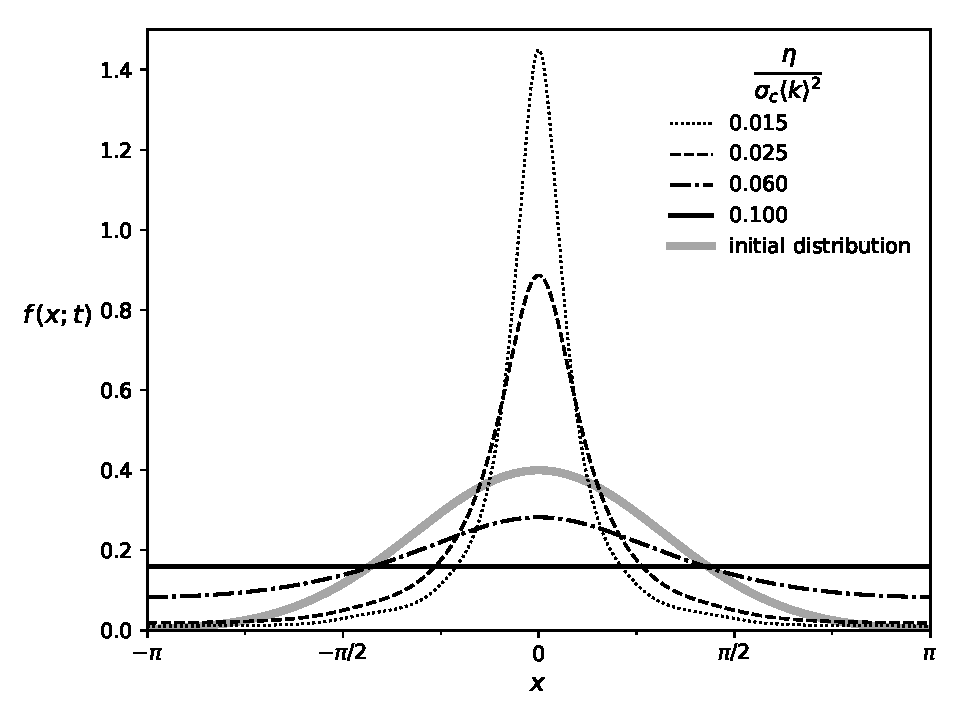
\includegraphics[width=0.7\linewidth]{figures/cont_mean_field_final_dist_BW}
	\caption{ The final state distribution $f(x;M\Delta t)$, for $M=3\cdot 10^5$ time steps, as a function of state $x$ for different values of the ratio $\frac{\eta}{\sigma_c\langle k \rangle^2}$ of system parameters. $M$ was large enough to ensure that the system converged to a stationary solution. The constant solution at $\frac{\eta}{\sigma_c\langle k \rangle^2} = 0.1$ is $f(x;t) = \frac{1}{2\pi}$. The system was initialised as a standard normal distribution (with zero mean and unit variance), however, note that the initial condition does not influence the outcome unless a stationary solution is chosen as initial condition.}
	\label{fig:cont_mean_field_final_dist}
\end{figure}

In order to verify that the final state distributions have converged (within certain numerical tolerance) to a stationary solution, the time evolution of the variance of the distribution $\sigma_f^2$ \footnote{Note that $\sigma_f^2$ is the variance of the state distribution $f(x;t)$ and $\sigma_c$ is the rate of three-body interactions.} is visualised in \cref{fig:cont_mean_field_var_vs_t}. After $\tau=300$ time steps, the variance has converged for almost all values of $\frac{\eta}{\sigma_c\langle k \rangle^2}$. In the situations where there was no convergence after 300 time steps, we verified that convergence of $\sigma_f^2$ was obtained at a later moment, before the end of the computation. If we combine this result with the fact that all feasible state distributions integrate to one on the state set $\Omega = (-\pi,\pi]$ and with the observation that the shape of the distribution remains the same in the last part of the simulation, we can conclude that the final distributions after $3\cdot 10^5$ time steps correspond to steady-state distributions. 

\begin{figure}[tbp]
	\centering
	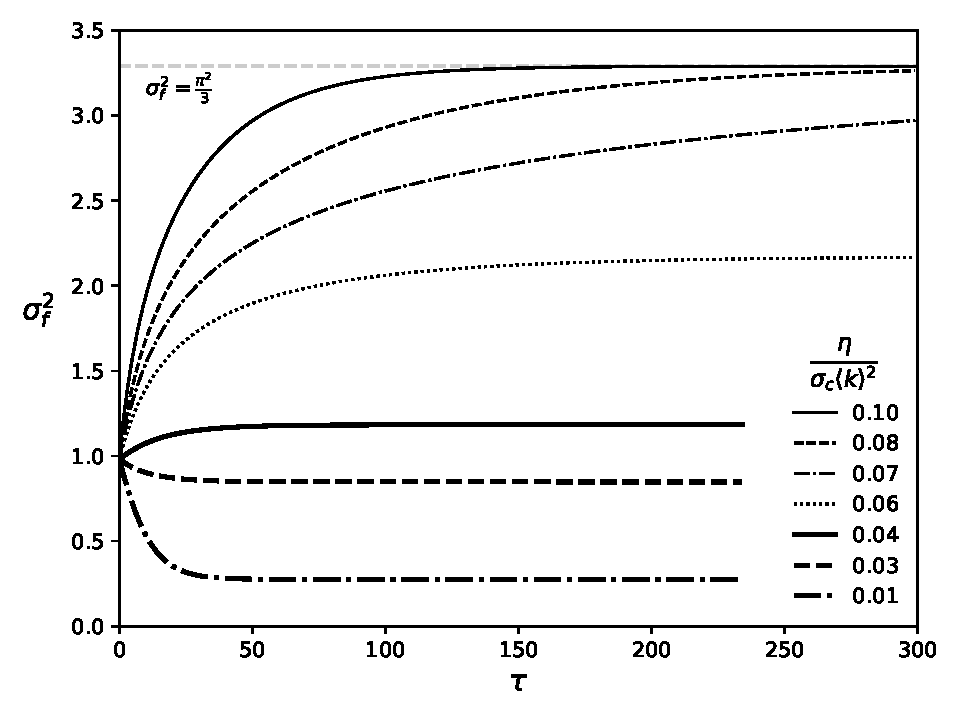
\includegraphics[width=0.7\linewidth]{figures/cont_mean_field_var_vs_t_BW}
	\caption{Time evolution of the variance $\sigma_f^2$ of the state distribution $f(x;t)$ for various values of $\frac{\eta}{\sigma_c\langle k \rangle^2}$. For almost all values of the system parameters convergence was achieved within 300 time steps. For $\frac{\eta}{\sigma_c\langle k \rangle^2} \in \{0.07, 0.08\}$ convergence was achieved at a later moment in the computation. $\sigma_f^2 = \frac{\pi^2}{3}$ corresponds to a uniform state distribution. The legend lists the curves from top to bottom. }
	\label{fig:cont_mean_field_var_vs_t}
\end{figure}

Comparing continuous state adaptive network models to the discrete state models, we have the following similarities. The disordered solution in which all possible states in $\Omega$ are equally distributed over all agents corresponds to the continuous uniform distribution. Furthermore, the ordered solution, in which there is one state occupied by a majority of nodes compared to all other states, is a bell-shaped distribution in the continuous case. In the limit to all nodes occupying the same state $f(x;t)$ becomes a Dirac delta distribution. In contrast to the discrete state networks, minority distributions do not have equal densities. We will use the variance of the distribution as a measure of the amount of order in the system. A system which is completely disordered is represented by a uniform distribution $f(x;t)=\frac{1}{2\pi}$, such that 
\begin{equation}
\sigma_f^2= \frac{1}{2\pi} \left[ \int\limits_{-\pi}^\pi dx\ x^2 - \left( \int\limits_{-\pi}^\pi dx\ x \right)^2 \right] = \frac{\pi^2}{3}.
\end{equation}
On the other hand, for a completely ordered system, which is represented by a Dirac delta distribution, we have $\sigma_f^2 \to 0$ by definition. Similar to the discrete state adaptive networks, the final state distribution depends on the ratio of system parameters. If there is a relatively high noise rate $\eta$, compared to $\sigma_c$ then the network tends to end up in a less ordered state compared to situations in which the rate $\sigma_c$ or the mean degree $\langle k \rangle$ is relatively high. In these latter cases, the system will evolve towards a more ordered distribution. We can make this quantitative by computing the variance of the stationary solution for multiple values of $\frac{\eta}{\sigma_c\langle k \rangle^2}$. The result is plotted in \cref{fig:cont_mean_field_variance_zoom}.

\begin{figure}[tbp]
	\centering
	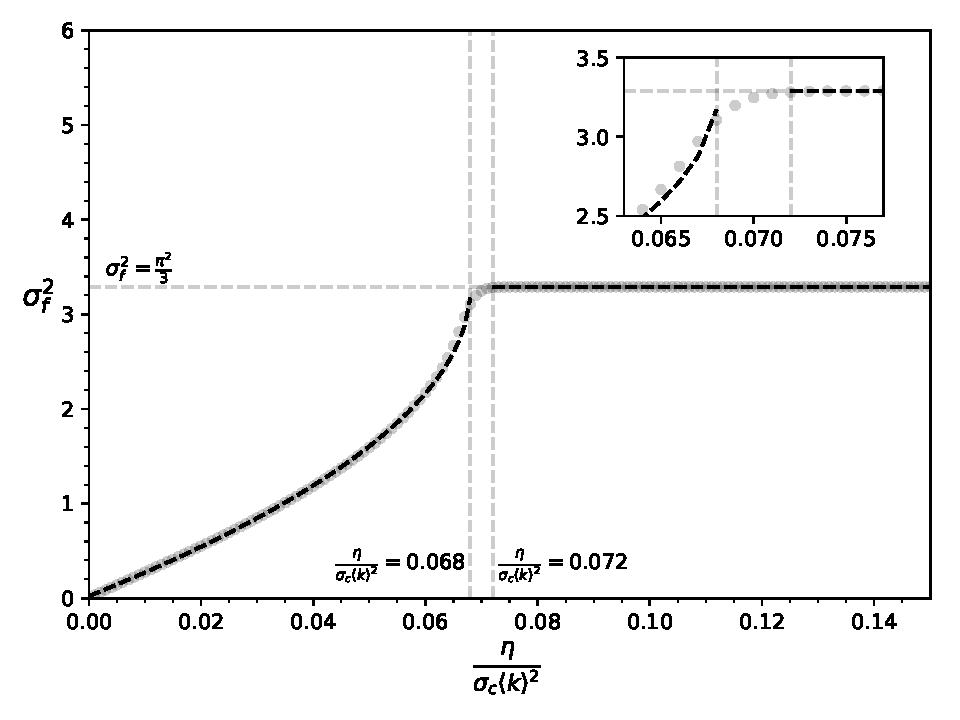
\includegraphics[width=0.7\linewidth]{figures/cont_mean_field_variance_zoom}
	\caption{Variance $\sigma_f^2$ of the stationary state of the state distribution $f(x;t)$ as function of the ratio $\frac{\eta}{\sigma_c\langle k \rangle^2}$ of mean field system parameters. The transition from a disordered to an ordered state occurs at $\frac{\eta}{\sigma_c\langle k \rangle^2} =0.068$. For $\frac{\eta}{\sigma_c\langle k \rangle^2} > 0.072$ the state distribution function is constant at $\frac{1}{2\pi}$ such that $\sigma_f=\frac{\pi^2}{3}$ and the system is completely disordered. For $\frac{\eta}{\sigma_c\langle k \rangle^2} < 0.068$ the state distribution has a maximum value for some state $x$, such that the system is ordered. On this interval, the black dashed line is a least squares fit of a square root function to all steady state variances $\sigma_f^2$. (Inset) A close up of the region in which the transition from the ordered to the disordered state occurs. The data points in this region do not fit the square root, nor the constant $\frac{\pi^2}{3}$. }
	\label{fig:cont_mean_field_variance_zoom}
\end{figure}

\begin{figure}[tbp]
	\centering
	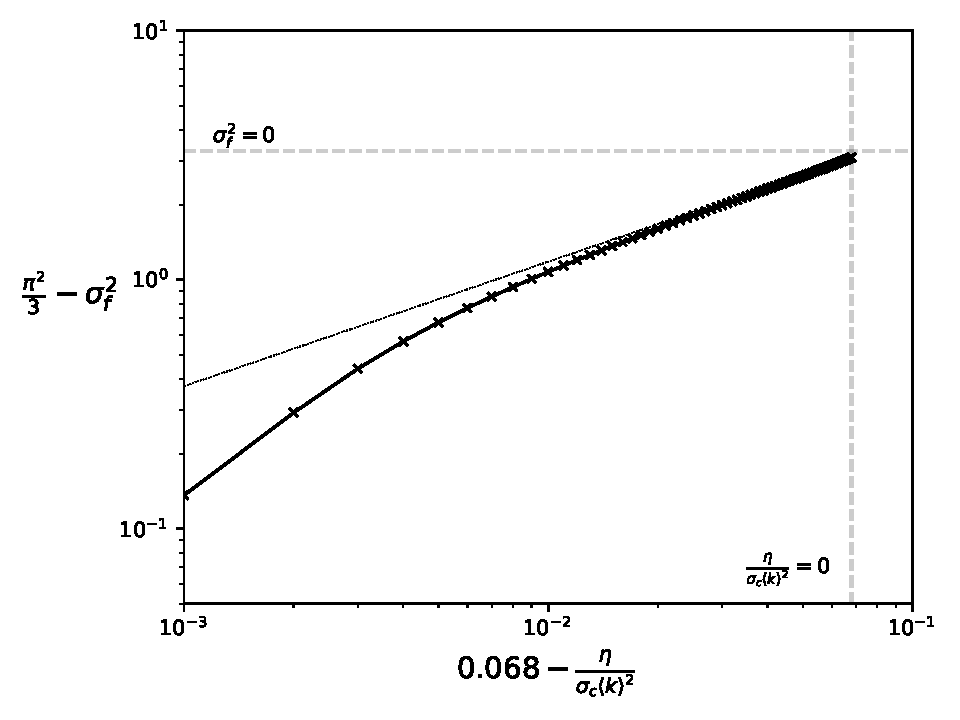
\includegraphics[width=0.7\linewidth]{figures/cont_mean_field_variance_loglog}
	\caption{Variance $\sigma_f^2$ of the stationary state of the state distribution $f(x;t)$ versus the ratio $\frac{\eta}{\sigma_c\langle k \rangle^2}$ of mean field system parameters on logarithmic scales. Only the ordered solutions $\left(\frac{\eta}{\sigma_c\langle k \rangle^2} < 0.068\right)$ were plotted. The dotted line has slope $\frac{1}{2}$, representing a square root function (with offset).}
	\label{fig:cont_mean_field_variance_loglog}
\end{figure}
\raggedbottom
For $\frac{\eta}{\sigma_c\langle k \rangle^2} > 0.072$ the variance $\sigma_f^2$ in the state distribution function $f(x;t)$ equals the expected variance for the disordered solution. For $\frac{\eta}{\sigma_c\langle k \rangle^2} < 0.068$ we have $\sigma_f^2 < \frac{\pi^2}{3}$, corresponding to a system in which one subset of states is more present than the others. These are the not-constant state distributions in \cref{fig:cont_mean_field_final_dist}. For discrete state networks, the density of a certain state as a function of the system parameters could be analytically expressed by a square root relationship \cite{Chen2016}. In order to check if a similar relation holds between the distribution variance and system parameters for the continuous state networks, the data points for $\frac{\eta}{\sigma_c\langle k \rangle^2} < 0.068$ are plotted on logarithmic scales in \cref{fig:cont_mean_field_variance_loglog}. Comparing the curve shape with the dotted square root function, we can see that especially for lower values of $\frac{\eta}{\sigma_c\langle k \rangle^2}$ the variances lie on a line with slope $\frac{1}{2}$, which is a property of a square root relation. Moreover, we can make a least squares fit of 
\begin{equation}
\sigma_f^2 = \frac{\pi^2}{3} - a \sqrt{0.068-\frac{\eta}{\sigma_c\langle k \rangle^2}}, \quad \text{for} \quad \frac{\eta}{\sigma_c\langle k \rangle^2} < 0.068, \qquad a \in \mathbb{R},
%[a,b]=[12.52327665,  0.0680888 ]
%np.pi**2/3 - a*np.sqrt(b - n)
%r2sqrt=  0.9991702860618208
\end{equation}
in \cref{fig:cont_mean_field_variance_zoom}. The optimal parameters is $a = 12.52$, with goodness of fit $R^2 = 0.999$. Hence we confirm that the relation is indeed given as a square root function. The variances for values $\frac{\eta}{\sigma_c\langle k \rangle^2} \in [0.068, 0.072]$ do not fit the least squares fit, nor the constant $\frac{\pi^2}{3}$. Hence, the transition from the ordered state to a disordered state occurs in this region. However, we can expect it to be closer to $0.068$, since this is where the fitted square root meets the variance of the disordered state. This is in line with the fact that systems with $\frac{\eta}{\sigma_c\langle k \rangle^2}$ close to the ratio at which the transition takes place tend to converge much slower than systems which have a much higher or lower ratio. This can also be observed in \cref{fig:cont_mean_field_var_vs_t}. It would mean that if we take both the simulation time and the number of grid points to infinity, we would have a perfect distinction between the disordered states on the branch where the variance is $\frac{\pi^2}{3}$ and the branch which can be described as a square root function. Taking everything together, the system ends up in an ordered state if $\frac{\eta}{\sigma_c\langle k \rangle^2} < 0.068$ and in a disordered state if $\frac{\eta}{\sigma_c\langle k \rangle^2}>0.068$, where convergence rates are very low for ratios close to $0.068$. 

Lastly, we check whether we can make a judicious guess for an analytic stationary solution which fits the simulation results. In the first place, it is not hard to see that 
\begin{equation}
f(x)=\frac{1}{2\pi}
\end{equation}
forms the disordered stationary solution.

One might expect the ordered state distribution to have a bell-shape. To check this, various final state distributions are plotted on a logarithmic scale versus the state $x$ on both linear and logarithmic scales in \cref{fig:cont_mean_field_linlog_loglog} to check if they can be represented by either renormalised Gaussian or renormalised Cauchy distributions. A Gaussian distribution is of the form
\begin{equation}
f(x; \mu_f, \sigma_f^2) = \frac{A}{\sqrt{2\pi\sigma_f^2}} \exp{\left(-\frac{(x-\mu_f)^2}{2\sigma_f^2}\right)},
\label{eq:gaussian_fit}
\end{equation}
in which $\mu_f$ represents the mean and $\sigma_f^2$ the variance of the distribution. This is an exponential function in $x^2$ and therefore it will appear as a parabola on a logarithmic-linear-plot. It is easy to see that the state distributions do not follow the shape of a parabola, from which we can conclude that the final distributions are not given as Gaussian distributions. The Cauchy distribution can be written as
\begin{equation}
f(x; x_0, \gamma) = \frac{A}{\pi \gamma} \frac{\gamma^2}{(x-x_0)^2+\gamma^2} 
\label{eq:cauchy_fit}
\end{equation}
with $A \in \mathbb{R}$ the amplitude, $x_0$ the location parameter, specifying the location of the maximum and $\gamma$ the scale parameter corresponding to the half-width at half-maximum. Supposing $x_0=0$, this distribution is a polynomial function in $x^2 + \gamma^2$, such that if it is plotted on a graph with logarithmic scales it will appear as a line with slope $-2$. \Cref{fig:cont_mean_field_linlog_loglog} shows that the final state distributions are very similar to Cauchy distributions, especially around $x=0$, the location of the peak of the distribution.
\begin{figure}[tbp]
	\centering
	\makebox[\textwidth][c]{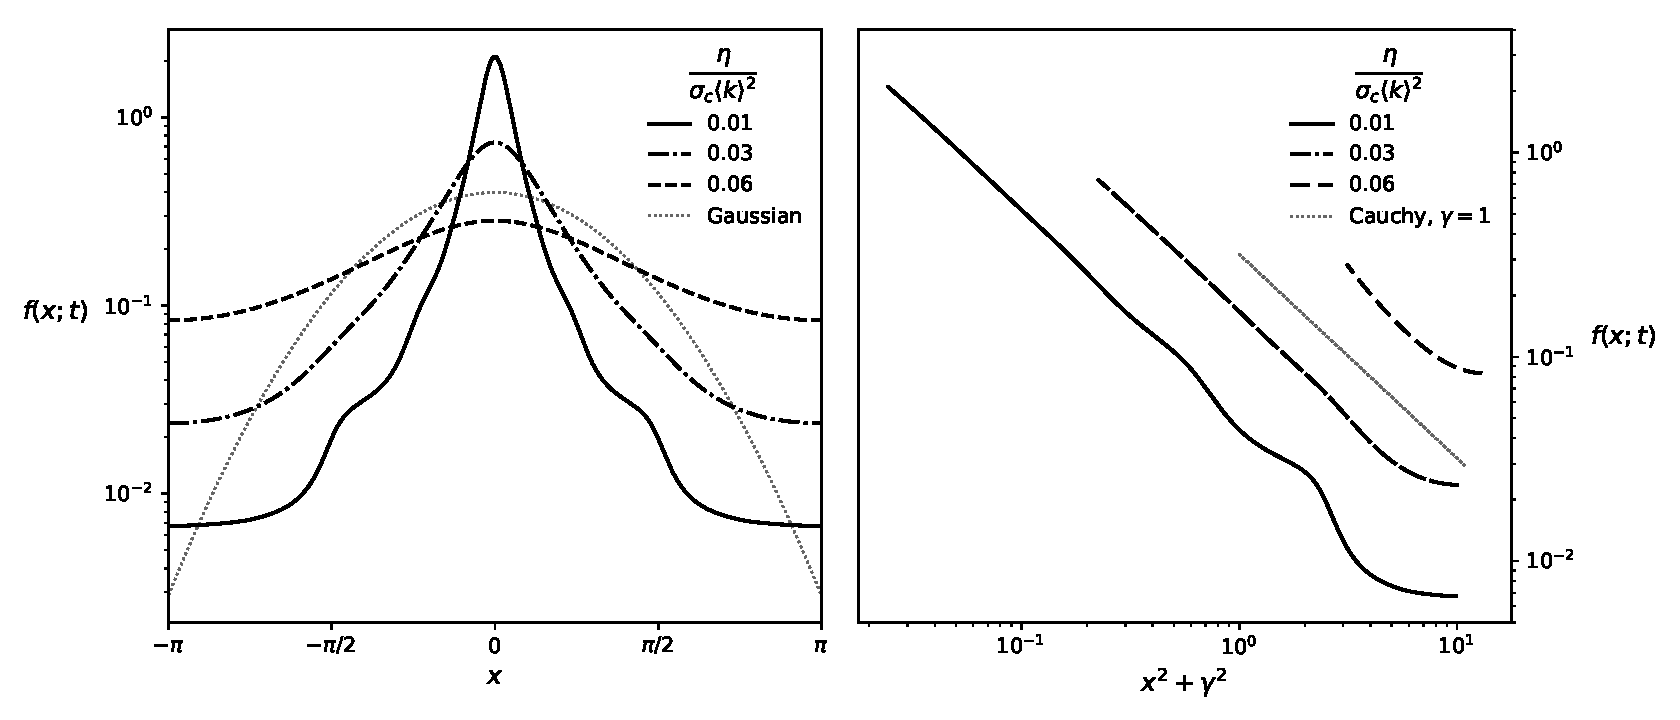
\includegraphics[width=1.2\linewidth]{figures/cont_mean_field_linlog_loglog}}%
	\caption{(left) The final state distribution function $f(x,M\Delta t)$ for $M=3\cdot 10^5$, for various values of $\frac{\eta}{\sigma_c\langle k \rangle^2}$, on logarithmic scale versus $x$ on linear scale. The dotted line represents a standard normal distribution. (right) The same final state distribution functions on logarithmic scale versus $x$ on logarithmic scale. The dotted line is the Cauchy distribution with $x_0=0$ and $\gamma=1$.}	
	\label{fig:cont_mean_field_linlog_loglog}
\end{figure}

To verify this, a least squares fit of a renormalised Gaussian distribution and a renormalised Cauchy distribution was made for various numerical final distributions. The results are plotted in \cref{fig:cont_mean_field_G_C_LSQ}. The least squares fit parameters, goodness of fit $R^2$ and area under the distribution are given in \cref{tab:fit_param_G_C_mean_field}. 
\begin{figure}[tbp]
	\centering
	\makebox[\textwidth][c]{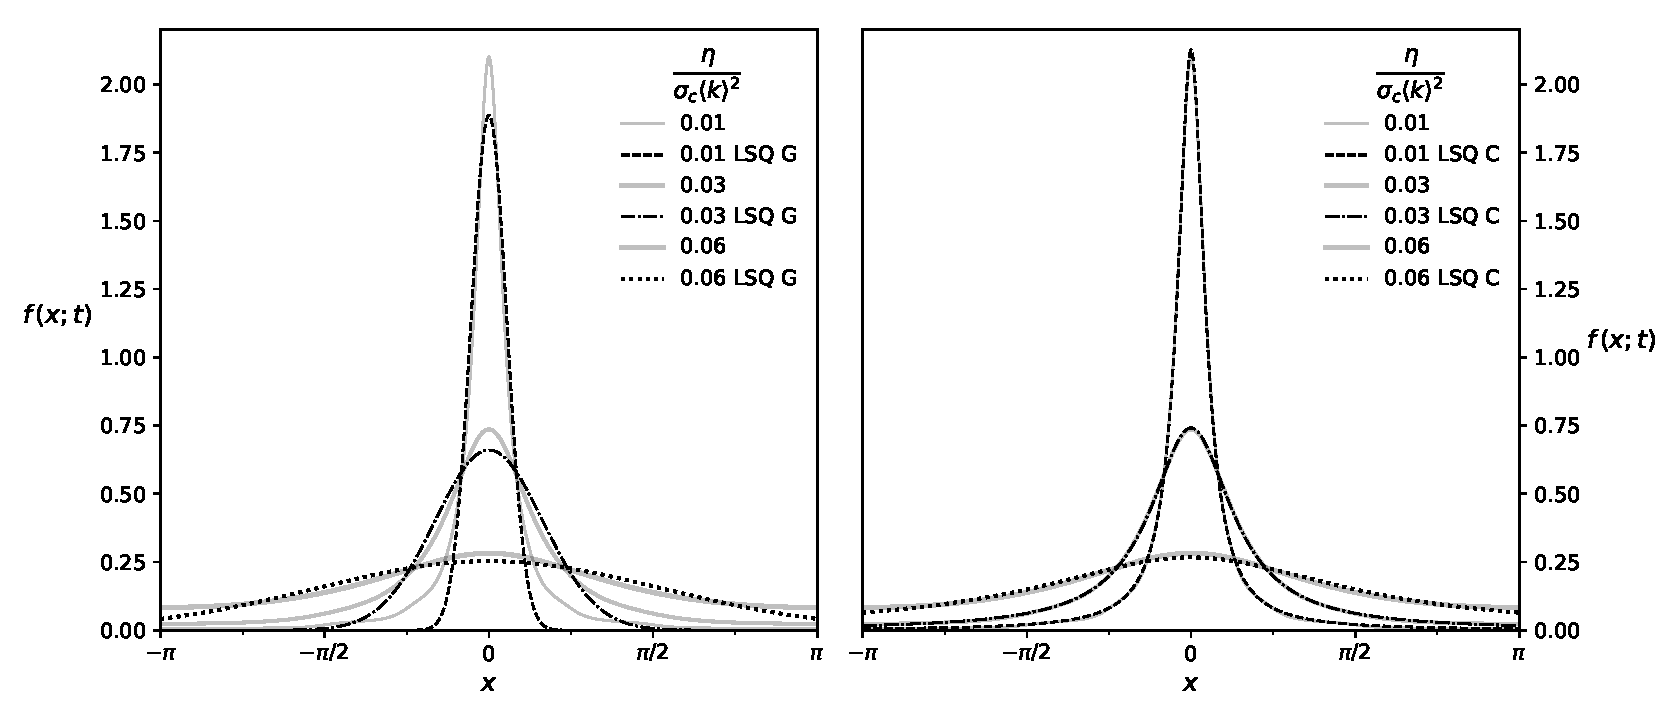
\includegraphics[width=1.2\linewidth]{figures/cont_mean_field_G_C_LSQ_BW}}%
	\caption{(soft curves) The final state distribution function $f(x,M\Delta t)$ for $M=3\cdot 10^5$, for various values of $\frac{\eta}{\sigma_c\langle k \rangle^2}$. (dashed/dotted curves, left) Least squares fits of the Gaussian distribution \cref{eq:gaussian_fit} to the final state distributions. (dashed,dotted curves, right) Least squares fits of the Cauchy distribution \cref{eq:cauchy_fit} to the final state distribution. The fit parameters and goodness of fit can be found in \cref{tab:fit_param_G_C_mean_field}. Legend entries are ordered from narrow to wide distributions.}	
	%		Model: Gaussian1D
	%		Inputs: ('x',)
	%		Outputs: ('y',)
	%		Model set size: 1
	%		Parameters:
	%		amplitude              mean               stddev      
	%		------------------ -------------------- ------------------
	%		1.8869199340983431 0.003931905699130531 0.1710214168889275 r^2 =  0.9702645006971661
	%		Model: Gaussian1D
	%		Inputs: ('x',)
	%		Outputs: ('y',)
	%		Model set size: 1
	%		Parameters:
	%		amplitude               mean               stddev      
	%		------------------ --------------------- ------------------
	%		0.6602437702220101 0.0039319056828550645 0.5157928158887003 r^2 =  0.9590595022517387
	%		Model: Gaussian1D
	%		Inputs: ('x',)
	%		Outputs: ('y',)
	%		Model set size: 1
	%		Parameters:
	%		amplitude              mean               stddev      
	%		------------------- -------------------- ------------------
	%		0.25310965580063377 0.003443017140767288 1.6525862408185896 r^2 =  0.9152246613834332
	%		Model: Lorentz1D
	%		Inputs: ('x',)
	%		Outputs: ('y',)
	%		Model set size: 1
	%		Parameters:
	%		amplitude             x_0                 fwhm       
	%		----------------- -------------------- ------------------
	%		2.126350006940973 0.003931891310500699 0.3127311371479785 r^2 =  0.9998347150194508
	%		Model: Lorentz1D
	%		Inputs: ('x',)
	%		Outputs: ('y',)
	%		Model set size: 1
	%		Parameters:
	%		amplitude              x_0                 fwhm       
	%		------------------ -------------------- ------------------
	%		0.7411141536424105 0.003928147410212121 0.9497871980512957 r^2 =  0.9998021024587377
	%		Model: Lorentz1D
	%		Inputs: ('x',)
	%		Outputs: ('y',)
	%		Model set size: 1
	%		Parameters:
	%		amplitude              x_0                 fwhm       
	%		------------------ -------------------- ------------------
	%		0.2669586944545997 0.003536080789641112 3.5380590656994206 r^2 =  0.981634500857006
	\label{fig:cont_mean_field_G_C_LSQ}
\end{figure}
\begin{table}[tbp]
	\caption{(a) Parameters $A$, $\sigma_f^2$ for the least squares Gaussian fits in the left graph of \cref{fig:cont_mean_field_G_C_LSQ}.  For all fits $\mu_f < 10^{-6}$. (b) Parameters $A$, $\gamma$ for the least squares Cauchy distribution fits in the right graph of \cref{fig:cont_mean_field_G_C_LSQ}, where $\gamma$ is scale parameter of the distribution. For all fits the location parameter $x_0 < 10^{-4}$. The goodness of fit $R^2$ and the area under the curve are denoted in the last two columns.}
	\label{tab:fit_param_G_C_mean_field}
	\begin{subtable}{.475\linewidth}
		\centering
		\caption{}
		\begin{tabular}{l|llll}
			$\frac{\eta}{\sigma_c\langle k \rangle^2}$ & $A$                        & $\sigma_f^2$               & $R^2$ & $\int\limits_{-\pi}^\pi dx\ f(x)$  \\ \hline
			$0.01$                      & 1.89                       & 0.0292                  & 0.9703 &	0.808\\
			$0.03$                      & 0.660                      & 0.266                   & 0.9591 &	0.852\\ 
			$0.06$                      & 0.253         			 & 2.73					   & 0.9152 &	0.987\\
		\end{tabular}
	\end{subtable}%
	\hfill
	\begin{subtable}{.475\linewidth}
		\centering
		\caption{}
		\begin{tabular}{l|llll}
			$\frac{\eta}{\sigma_c\langle k \rangle^2}$ & $A$    & $\gamma$   & $R^2$ &	$\int\limits_{-\pi}^\pi dx\ f(x)$   \\ \hline
			$0.01$                      & 2.12   & 0.1564 & 0.9998 & 1.01	\\
			$0.03$                      & 0.741  & 0.4750 & 0.9998 & 0.999	\\
			$0.06$                      & 0.267  & 1.769  & 0.9816 & 0.999	
		\end{tabular}
	\end{subtable}%
\end{table}

On the left-hand side of \cref{fig:cont_mean_field_G_C_LSQ}, we can clearly see that a Gaussian distribution does not fit the final state distribution well. For the sharpest peak, the fit is good anywhere where the distribution has a high slope, but the fit does not reach the peak value, nor is it high enough for $x$-values far from $x=0$. Hence, the area under the fitted distribution is less than 1, making it unfeasible. For wider distributions, the $R^2$ value increases, meaning that the fit quality is higher. But in these cases the maximum and minimum values are estimated too low. An analytic substitution of \cref{eq:gaussian_fit} in \cref{eq:cont_swarming_complete} using Maple 2018 verifies that a Gaussian is no steady state solution\footnote{We made an even extension of \cref{eq:gaussian_fit} at $x=-\pi$ and $x=\pi$ before substitution, to make sure the integrals are properly defined.}.

The right-hand side of \cref{fig:cont_mean_field_G_C_LSQ} shows the least squares fits of Cauchy distribution to the final state distributions. These curves seem to be a much better fit than the Gaussian distributions, an observation which can also be made quantitative by the goodness of fit $R^2$ in \cref{tab:fit_param_G_C_mean_field}. Furthermore, the area under the curves is very close to $1$, corresponding with feasible state distributions. However, a closer look at the distribution corresponding to $\frac{\eta}{\sigma_c\langle k \rangle^2} = 0.06$ shows that a Cauchy distribution might not be the perfect analytic description of the stationary state distribution.  Substitution of \cref{eq:cauchy_fit} confirms this last observation\footnote{Again an even extension was made to \cref{eq:cauchy_fit} before substitution.}. 

It should be remarked that both Gaussian and Cauchy distributions yield the constant value $\frac{1}{2\pi}$ if we take the limit of respectively the variance or the half-width at half-maximum to infinity before renormalising on $[-\pi,\pi)$. This corresponds to the distribution of the disordered system. Moreover, they converge to a Dirac distribution if we take the same limit to zero, corresponding to a perfectly ordered system. Therefore it might be worthwhile for further research to check whether all steady-state distributions, i.e. either disordered and ordered, can be described by another bell-shaped distribution with the same properties, where one allows for taking the limit cases $\sigma_f^2 \to \infty$ and $\sigma_f^2 \to 0$ or $\gamma \to \infty$ and $\gamma \to 0$. 

\section{Moment closure approximation on swarming systems}
The same rules and assumptions with which we defined a swarming system in \cref{section:applying_network_to_swarming} will be applied to the moment closure approximation of continuous state adaptive networks in this section. Afterwards, analysis and discussion of the results will follow. 

The system consisting of two coupled non-linear partial integro-differential equations which make an adaptive network model two dimensional collective motion in a swarm is written as 
\raggedbottom
\begin{subequations}
	\label{eq:cont_swarming_complete}\small
	\begin{adjustwidth}{-.5in}{-.5in} 
		\begin{align}
		\frac{\partial f(x;t)}{\partial t} =\ &
		\eta \left( \frac{1}{2\pi} - f(x;t) \right) \\
		& + \sigma_c\int\limits_{-\pi}^\pi dz \int\limits_0^{\pi/2} d \xi  \
		\Bigg[ 
		\frac{l(x-\xi ,z;t)\ l(z,x+\xi ;t)}{f(z;t)} - \frac{l(z-\xi ,x;t)\ l(x,z+\xi ;t)}{f(x;t)} 
		\Bigg] \nonumber  \\[15pt]
		\frac{\partial l(x,y;t)}{\partial t} = &
		\int\limits_{-\pi}^\pi dz \
		\Bigg{\{ }
		\frac{\eta}{2\pi} \left( l(x,z;t) + l(z,y;t) \right)  \\
		& \phantom{\int\limits_{-\pi}^\pi dz\ \sum}
		+\sigma_c \frac{l(y,z;t)\ l(z,-y+2x;t)}{f(z;t)}
		+\sigma_c \frac{l(x,z;t)\ l(z,-x+2y;t)}{f(z;t)} \nonumber\\
		& \phantom{\int\limits_{-\pi}^\pi dz\ \sum}
		-\sigma_c \frac{l(y,x;t)\ l(x,z;t)}{f(x;t)} 	 
		-\sigma_c \frac{l(x,y;t)\ l(y,z;t)}{f(y;t)} \nonumber \\
		& \phantom{\int\limits_{-\pi}^\pi dz\ \sum}
		+ \sigma_c\int\limits_0^{\pi/2} d \xi \    
		\Bigg[  
		\frac{l(y,z;t)\ l(z, x-\xi;t)\ l(z, x+\xi;t)}{f(z;t)^2}  + 
		\frac{l(x,z;t)\ l(z, y-\xi;t)\ l(z,y+\xi ;t)}{f(z;t)^2} \nonumber\\ 
		& \phantom{\int\limits_{-\pi}^\pi dz\ \sum \sigma_c\int\limits_0^{\pi/2} \ d \xi \sum }
		- \frac{l(y,x;t)\ l(x, z-\xi;t)\ l(x,z+\xi ;t)}{f(x;t)^2} - 
		\frac{l(x,y;t)\ l(y, z-\xi ;t)\ l(y, z+\xi ;t)}{f(y;t)^2} 
		\Bigg]	 \
		\Bigg{ \} } \nonumber\\
		&+ \alpha\ f(x;t)\ f(y;t) - 
		(2\eta+\beta)\ l(x,y;t). \nonumber
		\end{align}
	\end{adjustwidth}
\end{subequations}

\normalsize Here we assumed the discrete closure relation from \cite{Chen2016} to be applicable in the continuous state case. 
\normalfont

\subsection{Discretisation}
Similar to the mean field approximation, we will look for numerical solutions to the system of equations (\ref{eq:cont_swarming_complete}). A first step into solving this system numerically is discretising the time and state sets and transforming the partial integro-differential equations into partial \textit{difference} equations. This discretisation will be conducted in a similar manner compared to the mean field approximation model. That is, the continuous time $t = [0, T_{\text{max}}]$ at which the network evolution is considered will be partitioned into $M$ intervals of length $\Delta t$, such that the discrete time set is of the form 
\[ t_d= \{0, \Delta t, 2 \Delta t, ... , (\tau-1) \Delta t,  \tau\Delta t, ..., T_{\text{max}} - \Delta t, T_{\text{max}}  \}, \]
such that $M \Delta t = T_{\text{max}}$ and $\tau$ is the discrete time index. Furthermore, the state set $\Omega$ is partitioned into $N$ intervals of length $\Delta \omega$, such that $\Omega = [-\pi,\pi)$ is transformed into 
\[\Omega_d = \{-\pi, -\pi+\Delta\omega,...,-\pi+ (p-1) \Delta\omega, -\pi+ p \Delta\omega, ... \pi-\Delta\omega, \pi \}, \]
in which $N \Delta \omega = 2\pi$ and $p$ is the discrete state index.

To keep things clear, we will use the following shorthand notation in the discretisation of the density functions $f$ and $l$ on the discrete state-time-grid. 

\begin{equation}
f_{p}^{\tau } = f(-\pi+p\Delta \omega; \tau \Delta t) \qquad l_{p,q}^{\tau }=l(-\pi+p\Delta\omega,-\pi+q\Delta\omega;\tau \Delta t).
\end{equation}
The grid on which $f_{p}^{\tau}$ is defined is visualised in \cref{fig:grid_pde}. For $l_{p,q}^\tau$ we have something similar, but then on a three-dimensional grid. Again the forward difference method is applied to discretise the partial derivatives, such that for the state distribution $f$ we have \cref{eq:forward_difference_f}, whilst for the link distribution $l$ we have
\begin{equation}
\frac{\partial}{\partial t}\ l(x,y;t) \approx \frac{l(x,y;t+\Delta t) - l(x,y;t)}{\Delta t} = \frac{l_{p,q}^{\tau+1} - l_{p,q}^{\tau}}{\Delta t},
\end{equation}
for $x = -\pi + p \Delta \omega $ and $y = -\pi + q \Delta \omega $. Once again, we take the left Riemann sums as discretisation for the integrals, just as in \cref{eq:left_riemann}. Taking everything together, the system of partial difference equations describing a continuous state adaptive network becomes

\begin{subequations}\label{eq:cont_swarming_complete_forward_Euler}
	\begin{alignat}{2}
	\frac{f_{p}^{\tau +1} - f_{p}^{\tau }}{\Delta t} = & 
	\ \eta \left(\frac{1}{2\pi} - f_{p}^{\tau } \right) + 
	\sigma_c\ \Delta\omega^2 \sum\limits_{j=0}^{N-1}\sum\limits_{i=0}^{\frac{N}{4}-1}  
	\Bigg(
	\frac{l_{p-i,j}^{\tau }\  l_{j,p+i}^{\tau }}{f_{j}^{\tau }} - 
	\frac{l_{j-i,p}^{\tau }\ l_{p,j+i}^{\tau }}{f_{p}^{\tau }} 
	\Bigg)\\[15pt]
	\frac{l_{p,q}^{\tau +1} - l_{p,q}^{\tau }}{\Delta t} = & 
	\sum\limits_{j=0}^{N-1} \Delta \omega 
	\Bigg[
	\frac{\eta}{2\pi} \left( l_{p,j}^{\tau } + l_{j,q}^{\tau }\right) \\
	& \phantom{\sum\limits_{j=0}^{N-1} \Delta \omega\sum\limits_{j=0}^{N-1} } 
	+ \sigma_c \frac{l_{q,j}^{\tau}\ l_{j,-q+2p}^{ \tau}}{f_{j}^{\tau}}
	+ \sigma_c \frac{l_{p,j}^{\tau}\ l_{j,-p+2q}^{ \tau}}{f_{j}^{\tau}}
	- \sigma_c \frac{l_{q,p}^{\tau }\ l_{p,j}^{\tau }}{f_{p}^{\tau }} 
	- \sigma_c \frac{l_{p,q}^{\tau }\ l_{q,j}^{\tau }}{f_{q}^{\tau }} \nonumber  \\
	& \phantom{\sum\limits_{j=0}^{N-1} \Delta \omega\sum\limits_{j=0}^{N-1} } 
	+ \sigma_c\ \Delta \omega \sum\limits_{i=0}^{\frac{N}{4}-1}  
	\Bigg(
	\frac{l_{q,j}^{\tau }\ l_{j, p-i}^{\tau }\ l_{j, p+i}^{\tau }}{(f_{j}^{\tau })^2}
	+ \frac{l_{p,j}^{\tau }\ l_{j, q-i}^{\tau }\ l_{j, q+i}^{\tau }}{(f_{j}^{\tau })^2}	\nonumber \\
	& \phantom{\sum\limits_{j=0}^{N-1}\sum\limits_{j=0}^{N-1} \Delta \omega \sigma_c\sum\limits_{i=0}^{\frac{N}{4}-1} \Delta \omega\sum }
	- \frac{l_{q,p}^{\tau }\ l_{p, j-i}^{\tau }\ l_{p,j+i}^{\tau }}{(f_{p}^{\tau })^2}
	- \frac{l_{p,q}^{\tau }\ l_{q, j-i}^{\tau }\ l_{q,j+i}^{\tau }}{(f_{q}^{\tau })^2}
	\Bigg)
	\Bigg] \nonumber \\
	&+ \alpha\ f_{p}^{\tau }\ f_{q}^{\tau }
	- (2\eta+\beta)\ l_{p,q}^{\tau }.\nonumber
	\end{alignat}
\end{subequations}
This system of equations can be rewritten as a forward Euler scheme, allowing for numerically computing the time evolution in any appropriate computing language, given feasible initial conditions.



\subsection{Results and discussion}
The forward Euler scheme of \cref{eq:cont_swarming_complete_forward_Euler} was implemented in Python. The input parameters of the script are the system parameters $\eta$, $\sigma_c$, $\alpha$ and $\beta$, step size $\Delta t = \frac{1}{400}$, and grid spacing $\Delta \omega = \frac{2\pi}{23}$. To generate results the system was solved for five different initial conditions (before normalisation): $\mathcal{N}(0,5)$, $\mathcal{N}(0,1)$ and  $\frac{1}{2\pi}+a\, \cos(x)$, for $a\in\left\lbrace\frac{1}{10}, \frac{1}{40}, \frac{1}{400}\right\rbrace$.  $\mathcal{N}(\mu,\sigma_f^2)$ indicates the normal distribution with mean $\mu$ and variance $\sigma_f^2$.

The link distribution function is initialised as 2-dimensional standard normal distribution. That is 
\begin{equation}\label{eq:IC_link}
	l(x,y;0)=\frac{1}{2\pi} \exp\left(-\frac{1}{2} \left(x^2+y^2\right) \right).
\end{equation} 
Similar to the discrete state models and the continuous state mean field approximation, the solution converges to a disordered solution if the ratio of the noise rate $\eta$ to the three-body interaction rate $\sigma_c$ is high enough. For this case, the state distribution function $f(x;t)$ is plotted for two different initial conditions in \cref{fig:cont_closure_state_t_disordered_IC1_IC6_s4}. If this rate is low enough the system converges to an ordered solution, which is visualised in \cref{fig:cont_closure_invertingbehaviour_IC2_IC3_s7} for two different initial conditions. For most initial conditions, the time evolution is similar to the graph on the left-hand side and is as expected. The graph on the right-hand side shows a phenomenon which was not encountered before; the highest density states at $\tau=0$ converge to a density of 0, whilst the lower density states end up dominating the system. This behaviour is most likely caused by the discretisation of the system. For example, if in the first time step the change in the peak value of the state distribution is bigger than $-2a=-\frac{1}{200}$ the distribution at $\tau=1$ will be inverted. If the change in consecutive time steps is smaller, then convergence to an inverted ordered state can be explained. One can check if this is really the case by testing if similar results are obtained when smaller time steps and more grid points in $\Omega$ are taken. 

\begin{figure}[tbp]
	\centering
	\makebox[\textwidth][c]{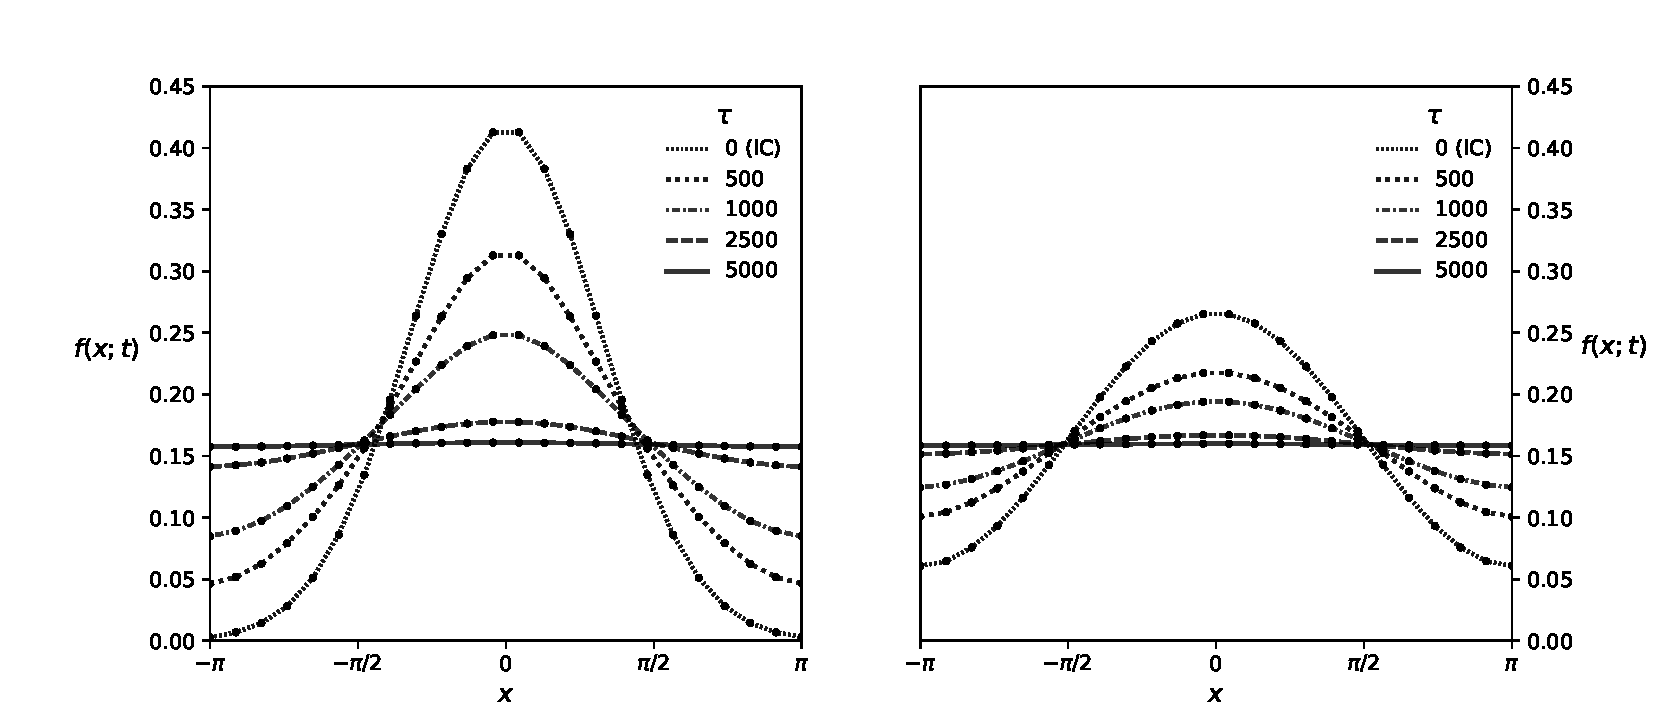
\includegraphics[width=1.2\linewidth]{figures/cont_closure_state_t_disordered_IC1_IC6_s4}}%
	\caption{The state distribution function $f(x;\tau \Delta t)$ for various values of $\tau$. The system parameters are $\eta=1$, $\sigma_c =4$, $\alpha=0.1$, $\beta=0.1$. The initial condition (IC) was taken as $f(x;0)~=~\mathcal{N}(0,1)$ (left) and $f(x;0)~=~\frac{1}{2\pi}+\frac{1}{10} \cos(x)$ (right). Both solutions converge to the disordered stationary solution. Grid points are indicated with dots.}
	\label{fig:cont_closure_state_t_disordered_IC1_IC6_s4}
\end{figure}

\begin{figure}[tbp]
	\centering
	\makebox[\textwidth][c]{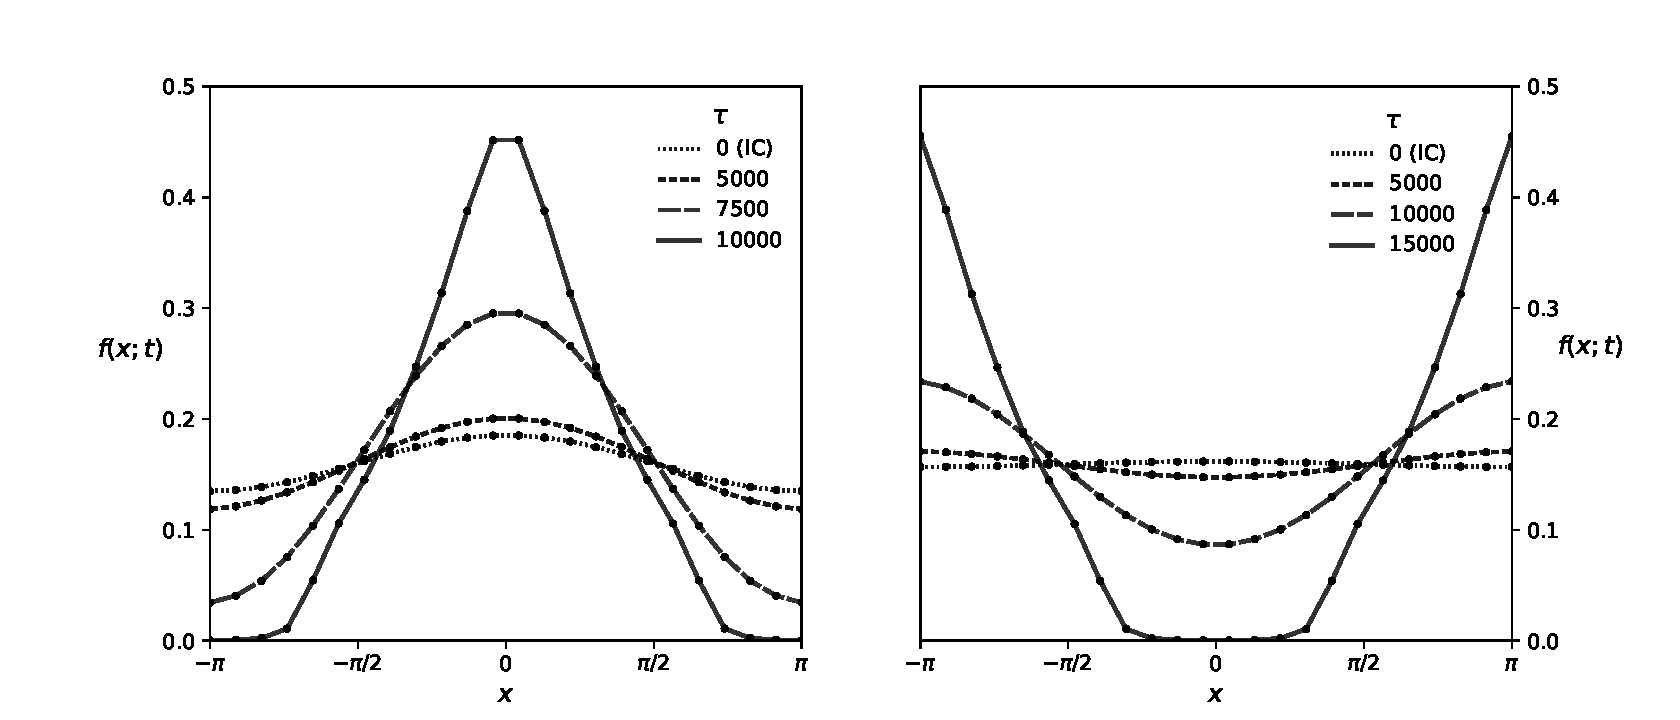
\includegraphics[width=1.2\linewidth]{figures/cont_closure_invertingbehaviour_IC2_IC3_s7}}%
	\caption{The state distribution function $f(x;\tau \Delta t)$ for various values of $\tau$. The system parameters are $\eta=1$, $\sigma_c =7$, $\alpha=0.1$, $\beta=0.1$. The initial condition (IC) was taken as $f(x;0)~=~\frac{1}{2\pi}+\frac{1}{40} \cos(x)$ (left) and $f(x;0)~=~\frac{1}{2\pi}+\frac{1}{400} \cos(x)$ (right). Both solutions converge to an ordered stationary solution. Grid points are indicated with dots.}
	\label{fig:cont_closure_invertingbehaviour_IC2_IC3_s7}
\end{figure}

As with the mean field approximation, we use the variance $\sigma_f^2$ of the state distribution as a measure for the amount of order in the system. In \cref{fig:cont_closure_variance_vs_sigma} the variance of the final distribution $f(x;M\Delta t)$ after $M=2\cdot 10^4$ time steps was plotted as function the ratio of system parameters $\frac{\eta}{\sigma_c}$ for all five initial conditions. For relatively high noise ratios $\left(\frac{\eta}{\sigma_c} \ge \frac{1}{5.2}\right)$ the system converges to the disordered solution and therefore $\sigma_f^2=\frac{\pi^2}{3}$. For a relatively low ratio $\left(\frac{\eta}{\sigma_c} \le \frac{1}{6.6}\right)$ the system converges to a disordered solution with nearly constant variance for all initial conditions. Note that this was not the case in the mean field approximation, where the final state distribution variance was depending on the system parameters by a square root relation. For $\frac{1}{6.6}\le\frac{\eta}{\sigma_c}\le\frac{1}{5.2}$ there is a bistable region, where the exact stationary solution depends on the initial condition. This may be a sign that the system has a subcritical (pitchfork) bifurcation at either of the two ends of the bistable region in combination with a saddle-node bifurcation at the other end. \Cref{fig:cont_closure_saddle_IC1_s5331} shows another sign of the presence of these bifurcations. The system initialised as standard normal distribution seems to converge to the disordered solution $f(x;t) = \frac{1}{2\pi}$ at first sight. However, after $\tau=7000$, the distribution stops flattening out and it starts converging to an ordered stationary solution, which is indicated by the star in \cref{fig:cont_closure_variance_vs_sigma}. This is an indication that the disordered solution forms a saddle-node for these parameters and the distribution gets close to the saddle-node in phase space before converging to its stable stationary solution. 
Note that we cannot determine the exact system parameters for which this bifurcation occurs with current solutions for only five different initial conditions. Further research is needed to determine the exact location and details of this bifurcation. Moreover, the exact reason why the \textit{ordered} state distribution has an almost constant variance for various values of the system parameters could be a subject of future research. 

\begin{figure}[tbp]
	\centering
	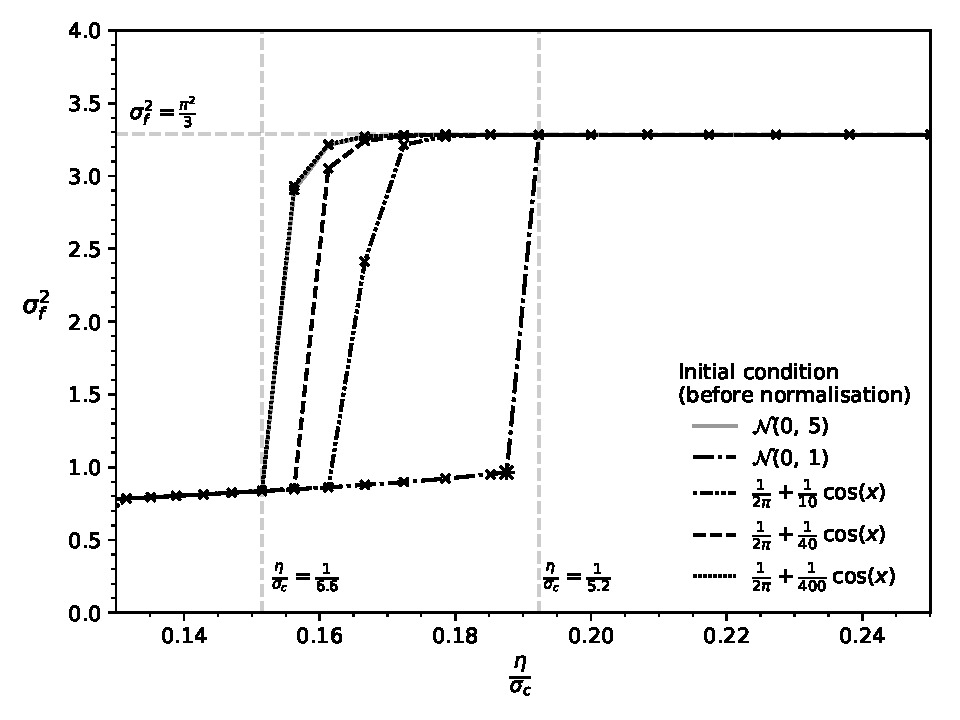
\includegraphics[width=0.7\linewidth]{figures/cont_closure_variance_vs_etaoversigma}%
	\caption{Variance $\sigma_f^2$ of the stationary state of the state distribution $f(x;t)$ as function of the ratio of system parameters $\frac{\eta}{\sigma_c}$ for various initial conditions. The system parameters were taken as $\eta=1$, $\alpha=0.1$,  $\beta=0.1$, $\sigma_c$ was varied. For $\frac{\eta}{\sigma_c}\ge\frac{1}{5.2}$ all distributions converged to the disordered stationary state solution, while for $\frac{\eta}{\sigma_c}\le\frac{1}{6.6}$ all distributions converged to an ordered solution. For $\frac{1}{6.6}\le\frac{\eta}{\sigma_c}\le\frac{1}{5.2}$ the stationary state solution depends on the chosen initial condition. The star indicates $\frac{\eta}{\sigma_c} = \frac{1}{5.331}$, for which the time evolution is plotted in \cref{fig:cont_closure_saddle_IC1_s5331}.}
	\label{fig:cont_closure_variance_vs_sigma}
\end{figure}

\begin{figure}[tbp]
	\centering
	\makebox[\textwidth][c]{\quad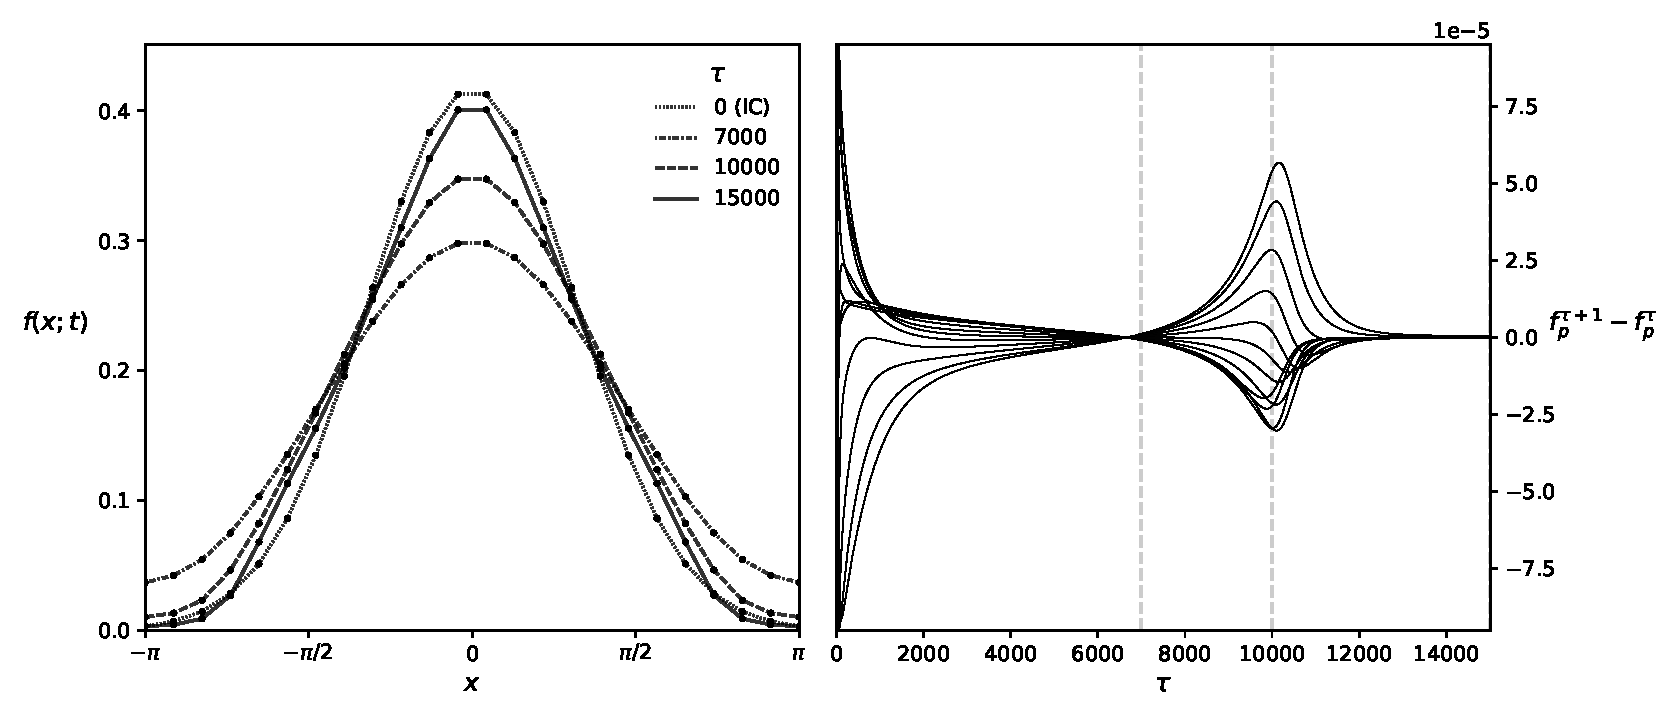
\includegraphics[width=1.2\linewidth]{figures/cont_closure_saddle_IC1_s5331}}%
	\caption{(left) The state distribution function $f(x;\tau \Delta t)$ for various values of $\tau$. The system parameters are $\eta=1$, $\sigma_c =5.331$, $\alpha=0.1$, $\beta=0.1$. The initial condition (IC) was taken as $f(x;0)~=~\mathcal{N}(0,1)$. Grid points are indicated with dots. (right) The difference $f_p^{\tau+1}-f_p^\tau$ between two consecutive state distribution functions for $p\in [0,...,11]$ versus the discrete time index $\tau$. Similar curves are obtained for $p\in [12,...,23]$ since the distribution is symmetric for all $\tau$. The distribution converged to a disordered solution, despite of the fact that it flattens out in the first 7000 time steps. }
	\label{fig:cont_closure_saddle_IC1_s5331}
\end{figure}


Some more remarks should be added about the (implementation of) the current numerical method which solves the system. More recommendations for future research will naturally follow. The most important limitation of the current script occurs when the ratio of the noise rate to the three-body interaction rate is taken too low $\left(\frac{\eta}{\sigma_c} \lesssim \frac{1}{8}\right)$. Then for some $\tau$, the distribution will get too narrow to be represented properly by $24$ grid points. That is, there is a time step after which the obtained curve is not smooth enough, introducing unacceptable numerical errors in consecutive time steps. Moreover, the smallest values of the state distribution function get so small, that extra numerical errors are obtained when these numbers get multiplied or divided by each other and by other numbers. Multiple things have been implemented to reduce these errors, amongst others calculating with 128-bit floating-point numbers, preventing division by small numbers, reducing the time step and implementing an implicit Euler backward integration method. These are however no permanent fixes for the problem. To resolve this issue permanently, one could find a way to increase the resolution of the state set $\Omega$ to more than $24$ grid points. This requires significant optimisation of the current computation time first. Moreover, one could look at alternative numerical methods to find stationary solutions, such as Newton-Raphson methods for systems of differential equations. The latter being rather a workaround than a solution since it does not allow for time evolution, but only for finding stationary solutions. If one finds higher resolution stationary state distributions, then it will be worthwhile to check whether the Cauchy distribution (or another bell-shaped distribution) can be the true analytic stationary solution to the system using more sophisticated PDE techniques.

Furthermore, future research could focus more on the link distribution function $l(x,y;t)$. That is, finding its steady state distributions, looking for bifurcations, investigating the influence of a different initial condition than \cref{eq:IC_link} and exploring the effect of different values for $\alpha$ and $\beta$. One could also do more research into how more sophisticated initial distributions evolve. This might be done by deriving and analysing a PDE for the change in the mean of the distribution
\begin{equation}
\frac{d}{dt} \langle x \rangle = \frac{\partial}{\partial t} \int\limits_\Omega dx\ x\ f(x;t)
\end{equation}
and by deriving and analysing the a PDE for change of the second moment
\begin{equation}
\frac{d}{dt} \langle x^2 \rangle = \frac{\partial}{\partial t} \int\limits_\Omega dx\ x^2\ f(x;t),	
\end{equation}
which is a measure for the amount of order in the system.

With all this information, the comparison between adaptive network models, other models for swarming systems and real life swarming systems can be made. Subsequently, one can find out how accurate adaptive network models are and where improvement might be needed. For example, it may be that adding other types of dynamics yields more accurate and realistic predictions. Finally, it will be interesting whether there are cases in which adaptive network models are better or more convenient than the current models.





\chapter{Conclusions and recommendations}

In this thesis, we considered adaptive network models with discrete and continuous state sets. The 2-state adaptive network models were analysed analytically and have two stationary points: an ordered and a disordered solution. The ordered solution, in which all states are equally distributed over all nodes, is stable for a relatively high dimensionless noise ratio compared to the dimensionless link creation ratio. The disordered solution, where one of the two states has a higher density than the other, is stable for relatively low dimensionless noise ratios. The transition from the ordered to the disordered state occurs through a supercritical pitchfork bifurcation. Numerical solutions are in line with these analytic results. Hence, irrespective of what biological, physical or social system the adaptive network is applied to, we know the outcome once the noise and link creation ratios are known. 

Furthermore, an adaptive network model was derived that works on a periodic or non-periodic continuous state set, obeying comparable dynamical rules as in the considered discrete state models. This model consists of a non-closed system of two coupled partial integro-differential equations, which can be analysed either in the mean field approximation or in the moment closure approximation. 

Both approximations were applied to a swarming system, consisting of two-dimensional motion of self-propelled particles with constant speed. Numerical solutions of the mean field model show that the disordered solution forms a stationary distribution if the noise rate is relatively high compared to the three-body interaction rate. For lower noise rates, the system ends up in an ordered solution, of which the variance is related to the system parameters by a square root function. A Cauchy distribution fits this ordered stationary solution very well, although it does not form an analytic stationary solution to the PDEs. Future research could focus on finding an analytic stationary ordered solution using more sophisticated PDE techniques.  

The moment closure approximation model was also numerically solved. Again, for relatively high noise rates compared to the three-body interaction rate the system ends up in a disordered solution. If the noise rate is relatively low, the system ends up in an ordered distribution, of which the variance does not spread as much as in the mean field approximation models and is probably not given by a square root function of the system parameters. There exists a bistable region in which the final distribution depends on the initial conditions of the system. This a sign of a subcritical pitchfork bifurcation in combination with a saddle-node bifurcation. Further research is needed to find the exact details of these bifurcations. Moreover, the current script solving the system numerically could be optimised, such that higher resolution solutions can be found for more different system parameters. These solutions could help in determining the exact form of the stationary solutions. Further research could also focus more on analysis the link distribution function and exploring the effect of different link creation and deletion rates and more sophisticated initial conditions. 

The comparison between continuous state adaptive networks, agent-based models and real-life swarming systems is still to be made. It will be very interesting to see whether the derived model can be an alternative to already existing models and what advantages and disadvantages there are. Moreover, there might be applications other than swarming systems that can be modelled very accurately as a continuous state adaptive network.

In the future, multiple possible extensions to the derived adaptive network model can be made. For example, one could do research into the effects of changing the interaction (rates) depending on the state a certain node occupies. These models may be a better representation of certain real-life situations. Another possibility is extending the concepts of adaptive networks with a stochastic component. In that case one would not be able to determine the complete time evolution beforehand.



%\textbf{Recommendations}

%\todo{arbitrary order, should be typed out}
%\begin{enumerate}
%	\item One could try finding analytic (stationary) solutions to the continuous model using more sophisticated PDE techniques.
%	\item The accuracy of the numerical integration scheme could be improved by implementing a more accurate discrete integration method, such as the trapezoidal rule. 
%	\item Significant improvements can be made in making the code more efficient. Indicate why this is necessary!
%	\item One could extend the concepts of adaptive networks with a stochastic component. With the described models, the complete time evolution is exactly known beforehand. This way, states which are initialised as a minority may end up in a majority.
%	\item One could do research into the effects of changing the interaction rates depending on the state a certain node occupies. That is, for example, nodes with a state in subset $S \subset \Omega$ have different rates (or obey completely different interactions) than nodes with a state in the complement $\Omega \setminus S$
%	\item One could do more research into the derived continuous state adaptive network model, for example how do more sophisticated initial distributions evolve. This might be done by deriving and analysing the change in the mean of the distribution
%	\begin{equation}
%	\frac{d}{dt} \langle x \rangle = \frac{\partial}{\partial t} \int_{-\pi}^\pi dx\ x\ f(x;t)
%	\end{equation}
%	and by deriving and analysing the change of the second moment
%	\begin{equation}
%	\frac{d}{dt} \langle x^2 \rangle = \frac{\partial}{\partial t} \int_{-\pi}^\pi dx\ x^2\ f(x;t),	
%	\end{equation}
%	which is a measure for the order in the system and the width of the distribution for various initial conditions.
%	\item One could compare the results to real-life swarming systems and agent-based models to check whether the continuous state adaptive network models might be better models than the current discrete state adaptive network models.
%	\item Applying continuous state adaptive networks to other systems than swarming systems.
%\end{enumerate}
%
		 
%\todo{numerieke probleem in het script zou zomaar eens niet oplosbaar kunnen zijn. De resultaten zijn opzich al goed nu. Het script preciezer maken kan zorgen dat de instabiliteit langer uitgesteld wordt. Dit kunnen bv dingen zijn zoals de trapezoidal rule gebruiken voor integratie en switchen naar float128, meer grid points, optimale thresholdwaarde vinden voor afkappen: zo klein mogelijk maar niet te klein dat we problemen krijgen etc. Of misschien overstappen naar een compleet ander numeriek schema. Er zou bijvoorbeeld gekeken kunnen worden naar of Newton-Raphson een oplossing biedt om de steady state oplossingen te vinden.}



\appendix			% resets chapter numbering, uses letters for chapter numbers and doesn't fiddle with page numbering;

\renewcommand\bibname{References}
\printbibliography

\end{document}
